%\documentclass[final,5p,times,twocolumn]{elsarticle}
%\documentclass[3pd]{elsarticle}
\documentclass{elsarticle}
 % The package hyperref provides LaTeX the ability to create hyperlinks within the document. Comment out the next line to load document onto the arXiv.
\usepackage{hyperref}
\usepackage{xcolor}

%\usepackage{draftwatermark}

% Use the option doublespacing or reviewcopy to obtain double line spacing
% \documentclass[doublespacing]{elsart}

%\documentclass[<options>]{elsarticle}
%where the options can be the following:
%(1) preprint ? default option which formats the document for submission to
%Elsevier journals. 
%(2) review ? similar to preprint option, but increases the baselineskip to facilitate easier review process.
%(3) 1p ? formats the article to the look and feel of the final format of model 1+ journals. This is always single column style.
%(4) 3p ? formats the article to the look and feel of the final format of model 3+ journals. If the journal is a two column model, use twocolumn option in combination.
%(5) 5p ? formats for model 5+ journals. This is always two column style.
% etc., see http://www.elsevier.com/framework_authors/misc/elsdoc.pdf

% if you use PostScript figures in your article
% use the graphics package for simple commands      
%\usepackage{graphics}
% or use the graphicx package for more complicated commands
\usepackage{graphicx}

% The amssymb package provides various useful mathematical symbols
\usepackage{amssymb}
% The amsmath package provides miscellaneous enhancements for improving the information structure and printed output of documents that contain mathematical formulas.
\usepackage{amsmath}
% The amsthm package provides an enhanced version of LATEX?s \newtheorem command for defining theorem-like environments. 
%\usepackage{amsthm}
\usepackage{multirow}
\newcommand\EatDot[1]{}

% The package lineno adds line numbers to LaTeX documents.
\usepackage{lineno}

\begin{document}  

\def \cebaf {{\textsc{cebaf}}}
\def \GX    {{\textsc{GlueX}}}
\def \gx    {{\textsc{GlueX}}}
\def \jlab  {{JLab}}

  
\begin{frontmatter} 

% Title, authors and addresses   

\title{The GlueX Beam Line and Detector}

% authors for GlueX overall NIM paper

\author[fsu]{H.~Al Ghoul}
\author[uofa]{E.~G.~Anassontzis}
\author[cmu]{A.~Austregesilo}
\author[jlab]{F.~Barbosa}
\author[uconn]{A.~Barnes}
\author[uofr]{T.~D.~Beattie}
\author[iu]{D.~W.~Bennett}
\author[mephi]{V.~V.~Berdnikov}
\author[uncw]{T.~Black}
\author[fiu]{W.~Boeglin}
\author[gwu]{W.~J.~Briscoe}
\author[usm]{W.~K.~Brooks}
\author[fsu]{B.~E.~Cannon}
\author[itep]{O.~Chernyshov}
\author[jlab]{E.~Chudakov}
\author[fsu]{V.~Crede}
\author[jlab]{M.~M.~Dalton}
\author[jlab]{A.~Deur}  
\author[nw]{S.~Dobbs}
\author[itep]{A.~Dolgolenko}
\author[asu]{M.~Dugger}
\author[gsi]{R.~Dzhygadlo}
\author[jlab]{H.~Egiyan}
\author[fsu]{P.~Eugenio}
\author[mit]{C.~Fanelli}
\author[gwu]{S.~Fegan}
\author[uofr]{A.~M.~Foda}
\author[iu]{J.~Frye}
\author[jlab]{S.~Furletov}
\author[uncw]{L.~Gan}
\author[ncatsu]{A.~Gasparian}
\author[itep]{A.~Gerasimov}
\author[yerevan]{N.~Gevorgyan}
\author[gsi]{K.~Goetzen}
\author[itemp]{V.~S.~Goryachev}
\author[fiu]{L.~Guo}
\author[usm]{H.~Hakobyan}
\author[mit]{J.~Hardin}
\author[fsu]{A.~Henderson}
\author[uofr]{G.~M.~Huber}
\author[glasgow]{D.~G.~Ireland}
\author[jlab]{M.~M.~Ito}
\author[cmu]{N.~S.~Jarvis}
\author[uconn]{R.~T.~Jones}
\author[yerevan]{V.~Kakoyan}
\author[fiu]{M.~Kamel}
\author[jlab]{C.~Keith}
\author[cua]{F.~J.~Klein}
\author[gsi]{R.~Kliemt}
\author[uofa]{C.~Kourkoumeli}
\author[usm]{S.~Kuleshov}
\author[tomsk]{I.~Kuznetsov}
\author[iu]{M.~Lara}
\author[umass]{I.~Larin}
\author[jlab]{D.~Lawrence}
\author[cmu]{W.~I.~Levine}
\author[glasgow]{K.~Livingston}
\author[uofr]{G.~J.~Lolos}
\author[tomsk]{V.~Lyubovitskij}
\author[jlab]{D.~Mack}
\author[jlab]{P.~T.~Mattione}
\author[itep]{V.~Matveev}
\author[jlab]{M.~McCaughan}
\author[cmu]{M.~McCracken}
\author[cmu]{W.~McGinley}
\author[uconn]{J.~McIntyre}
\author[usm]{R.~Mendez}
\author[cmu]{C.~A.~Meyer}
\author[umass]{R.~Miskimen}
\author[iu]{R.~E.~Mitchell}
\author[uconn]{F.~Mokaya}
\author[asu]{K.~Moriya}
\author[gsi]{F.~Nerling}
\author[mephi]{G.~Nigmatkulov}
\author[uofr]{N.~Ochoa}
\author[fsu]{A.~I.~Ostrovidov}
\author[uofr]{Z.~Papandreou}
\author[mit]{M.~Patsyuk}
\author[ncatsu]{R.~Pedroni}
\author[jlab]{M.~R.~Pennington}
\author[jlab]{L.~Pentchev}
\author[gsi]{K.~J.~Peters}
\author[jlab]{E.~Pooser}
\author[uconn]{B.~Pratt}
\author[jlab]{Y.~Qiang\fnref{f1}}
\fntext[f1]{Current address: Toshiba Medical Research Institute USA, Inc., 706 N Deerpath Dr, Vernon Hills, IL 60061.}
\author[fsu]{J.~Reinhold}
\author[asu]{B.~G.~Ritchie}
\author[nw]{L.~Robison}
\author[mephi]{D.~Romanov}
\author[nsu]{C.~Salgado}
\author[jlab]{N.~Sandoval}
\author[cmu]{R.~A.~Schumacher}
\author[gsi]{C.~Schwarz}
\author[gsi]{J.~Schwiening}
\author[uofr]{A.~Yu.~Semenov}
\author[uofr]{I.~A.~Semenova}
\author[nw]{K.~K.~Seth}
\author[iu]{M.~R.~Shepherd}
\author[jlab]{E.S.~Smith\corref{cor}}
\cortext[cor]{Corresponding author: Tel.: +1 757 269 7625.}
\ead{elton@jlab.org}
\author[cua]{D.~I.~Sober}
\author[jlab]{A.~Somov}
\author[mephi]{S.~Somov}
\author[usm]{O.~Soto}
\author[asu]{N.~Sparks}
\author[cmu]{M.~J.~Staib}
\author[jlab]{C.~Stanislav}
\author[wm]{J.~R.~Stevens}
\author[gwu]{I.~I.~Strakovsky}
\author[iu]{A.~Subedi}
\author[mephi]{V.~Tarasov}
\author[jlab]{S.~Taylor}
\author[uofr]{A.~Teymurazyan}
\author[mephi]{I.~Tolstukhin}
\author[nw]{A.~Tomaradze}
\author[usm]{A.~Toro}
\author[fsu]{A.~Tsaris}
\author[uofa]{G.~Vasileiadis}
\author[usm]{I.~Vega}
\author[cua]{N.~K.~Walford}
\author[glasgow]{D.~Werthm\"uller}
\author[jlab]{T.~Whitlatch}
\author[mit]{M.~Williams}
\author[jlab]{E.~Wolin}
\author[nw]{T.~Xiao}
\author[iu]{J.~Zarling}
\author[wuhan]{Z.~Zhang}
\author[jlab]{B.~Zihlmann}
\address[asu]{Arizona State University, Tempe, Arizona 85287, USA}
\address[uofa]{National and Kapodistrian University of Athens, 15771 Athens, Greece}
\address[cmu]{Carnegie Mellon University, Pittsburgh, Pennsylvania 15213, USA}
\address[cua]{Catholic University of America, Washington, D.C. 20064, USA}
\address[uconn]{University of Connecticut, Storrs, Connecticut 06269, USA}
\address[fiu]{Florida International University, Miami, Florida 33199, USA}
\address[fsu]{Florida State University, Tallahassee, Florida 32306, USA}
\address[gwu]{The George Washington University, Washington, D.C. 20052, USA}
\address[ghent]{Ghent University, Proeftuinstraat 86, B-9000 Ghent, Belgium}
\address[glasgow]{University of Glasgow, Glasgow G12 8QQ, United Kingdom}
\address[gsi]{GSI Helmholtzzentrum f\"ur Schwerionenforschung GmbH, D-64291 Darmstadt, Germany}
\address[iu]{Indiana University, Bloomington, Indiana 47405, USA}
\address[itep]{Institute for Theoretical and Experimental Physics, Moscow 117259, Russia}
\address[jlab]{Thomas Jefferson National Accelerator Facility, Newport News, Virginia 23606, USA}
\address[umass]{University of Massachusetts, Amherst, Massachusetts 01003, USA}
\address[mit]{Massachusetts Institute of Technology, Cambridge, Massachusetts 02139, USA}
\address[mephi]{National Research Nuclear University Moscow Engineering Physics Institute, Moscow 115409, Russia}
\address[nsu]{Norfolk State University, Norfolk, Virginia 23504, USA}
\address[ncatsu]{North Carolina A\&T State University, Greensboro, North Carolina 27411, USA}
\address[uncw]{University of North Carolina at Wilmington, Wilmington, North Carolina 28403, USA}
\address[nw]{Northwestern University, Evanston, Illinois 60208, USA}
\address[uofr]{University of Regina, Regina, Saskatchewan, Canada S4S 0A2}
\address[usm]{Universidad T\'ecnica Federico Santa Mar\'ia, Casilla 110-V Valpara\'iso, Chile}
\address[tomsk]{Tomsk State University, 634050 Tomsk, Russia}
\address[tomskb]{Tomsk Polytechnic University, 634050 Tomsk, Russia}
\address[yerevan]{A. I. Alikhanian National Science Laboratory (Yerevan Physics Institute), 0036 Yerevan, Armenia}
\address[wm]{College of William and Mary, Williamsburg, Virginia 23185, USA}
\address[wuhan]{Wuhan University, Wuhan, Hubei 430072, People's Republic of China}
\address[nc]{University of North Carolina at Wilmington, Wilmington, North Carolina 28403, USA}
\address[glasgow]{University of Glasgow, Glasgow G12 8QQ, United Kingdom}


%  
% \collaboration{The \sc{GlueX} Collaboration}
%



\begin{abstract}
***DRAFT place holder***\\
The GlueX experiment was designed to study photoproduction reactions with a 9-GeV linearly polarized beam. The energy and time of beam photons are tagged using a scintillator
hodoscope and scintillating fiber array. The flux is determined using a pair spectrometer and its polarization is determined using a triplet polarimeter. 
Charged particle tracks are analyzed in solenoidal field using a central straw tube
drift chamber and six packages planar chambers with cathode strips and drift wires. Electromagnetic showers are reconstructed in a cylindrical scintillating fiber calorimeter inside the magnet and
a lead glass array downstream. Charged particle identification is achieved by measuring energy loss in the wire chambers and using the flight time of particles between the target and outside 
detectors. The signals from all detectors are recorded with flash ADCs or pipeline TDCs into memories allowing trigger decisions with a latency of 4 $\mu$s. The detector operates routinely at
trigger rates of 50 kHz. We describe the photon beam, the GlueX detector components, electronics, data-acquisition and monitoring, and the performance of the system during the first three 
years of operation.
\end{abstract}   

%\begin{keyword}
% keywords here, in the form: keyword \sep keyword
% electromagnetic calorimeter \sep sampling calorimeter \sep scintillating fibers  \sep silicon photomultipliers \sep MPPC \sep GlueX
% PACS codes here, in the form: \PACS code \sep code
% \PACS 29.40.Mc \sep 29.40.Vj 
% \end{keyword}

\end{frontmatter}

% \linenumbers    
  
   

%===============================+================================
%============    Project Background  and Detector Requirements =============
%================================================================

\newpage 

\tableofcontents

%=======================+=========================
%================  Introduction  ================
%=================================================


\section[The \gx{} experiment (TCR)]{The \gx{} experiment \label{sec:gluexexperiment} }

The primary motivation of the \gx{} experiment is to search for and, ultimately, study the pattern of gluonic excitations in the meson spectra produced 
in $\gamma p$ collisions at 9~GeV~\cite{gluex-ref}. Specifically, GlueX aims to study the properties of hybrid mesons --- particles where the gluonic field 
contributes directly to the $J^{PC}$ quantum numbers of the mesons~\cite{meyer:2015eta}. 

\subsection[The Hall D complex]{The Hall D complex \label{sec:gluexexperiment:complex}}
The Hall D complex consists of a tagger hall where incident 12~GeV electrons produce
a beam of linearly polarized photons, and the experimental hall, where the photons interact
in an experimental target and the resulting interactions are recorded by the \GX{} detector.
A schematic of the complex, including the tagger area and the \GX{} experiment, is shown 
in Figure~\ref{fig:gluex_schematic}.
\begin{figure}[h!]\centering
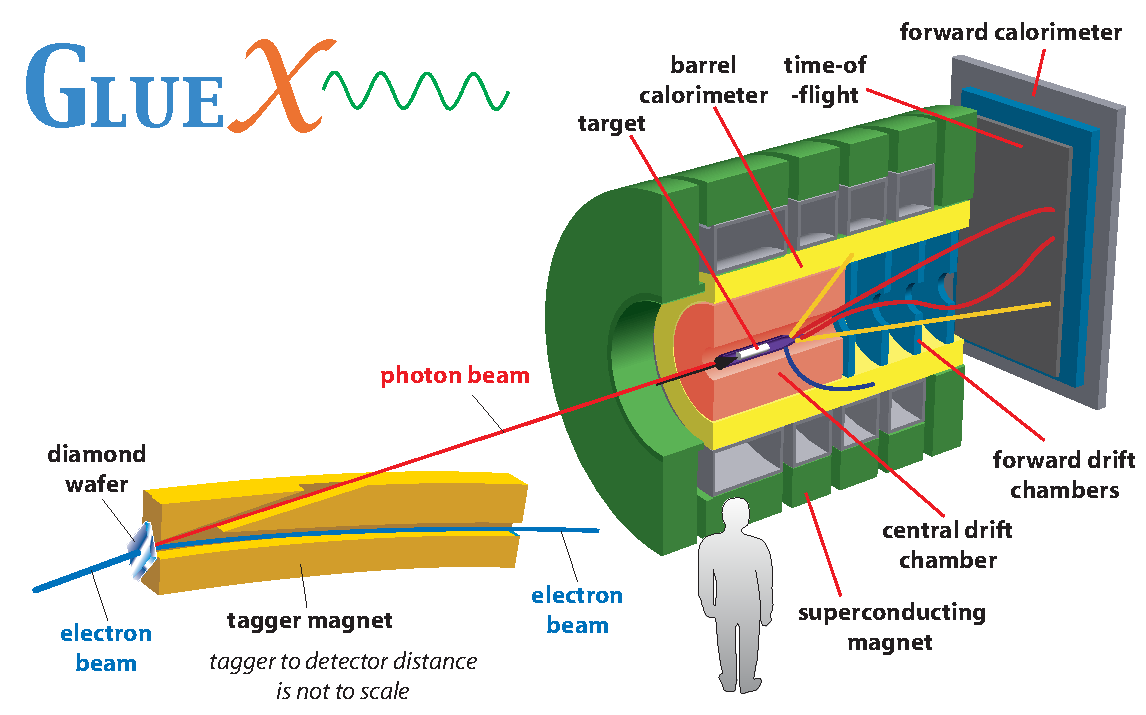
\includegraphics[width=0.9\textwidth]{../../apparatus/general/figs/GlueX_detector_labels_noplug}
\caption[]{\label{fig:gluex_schematic}A cut-away drawing of the \GX{} detector in Hall D.}
\end{figure}
More information on the production, tagging and monitoring of the photon beam can be found in
Chapter~\ref{sec:chap:beam}. The \GX{} detector is described in detail in 
Chapter~\ref{sec:hall-d-spectrometer}.
\mysubsection[Experimental Description]{Experimental Description}
\label{sec:intro:detector}
As seen in Figure~\ref{fig:gluex_schematic}, the 12~GeV electron beam passes through a 
thin diamond wafer, where bremsstrahlung photons are produced. The electrons are then deflected
by the tagger magnet. Non-radiating electrons are sent to a beam dump, while the electrons which
have radiated more than a half of their energy
are detected by a pair of hodoscope arrays. These arrays are aligned such that each detector element
maps onto a narrow momentum range in the deflected electrons, and hence, a narrow energy range
in the produced photons. Thus, the energy of each photon is ``tagged'' and known in  the experiment.
The photon beam then travels about $80\, m$ to the experimental hall, where prior to entering the
experiment, it is collimated, and monitored using both a polarimeter and a pair spectrometer.

The photons can then interact in the target in \GX{}. Much of the experimental apparatus is inside
a solenoidal magnet with central field of 2~T. The charged particles produced by the interacting
photons are tracked by the start counter immediately outside the target (not shown in the figure),
and then a pair of tracking systems. The central drift chamber is based on 28 layers of axial and stereo
straws. The forward drift chambers are 24 drift chambers planes with both cathode
and anode readout.  The flight-time of charged
particles are measured using a combination of the start counter and the time-of-flight wall in the forward
direction, and the start counter and the barrel calorimeter inside the solenoid.

The final-state photons are detected in a pair of calorimeters. The barrel calorimeter, located inside the 
solenoid, consists if layers of scintillating fiber alternating with lead sheets. The forward calorimeter
is downstream of the time-of-flight wall, and consists of $2800$ lead-glass blocks. 

\subsection[Experimental Requirements]{Experimental Requirements \label{sec:intro:requirements}}
In order to be able to exclusively reconstruct events with final states given in Table~\ref{tab:exotic_modes},
accurate reconstruction of the incident photon, as well as the produced charge particles and photons
is necessary. 

The linear polarization of the incident photon beam is produced through the coherent 
bremsstrahlung process. These coherent photons have energies in the range of 8.4 to 9~GeV,
and will be about $40\%$, after the beam collimation to $\sim{}25~\mu$rad with respect to the incoming 
electron direction. For these linearly-polarized photons, it is necessary to accurately know the photon 
energy, both for the exclusive final state reconstruction and also to accurately determine the photon 
polarization on an event-by-event basis. In \GX{}, this energy is known to an accuracy of $0.1\%$ of the
incident photon energy.

In order to exclusively reconstruct multi-particle final states, the \GX{} detector needs be nearly
hermetic with good momentum and energy resolution for both charged particles and photons.
In order to be able to carry out the needed amplitude analysis, the detector acceptance  needs to 
be reasonably uniform, and well understood and modeled in simulation. Typical momentum resolution
for charged particles $1$--$2\%$, while for very-forward high-momentum particles, it is somewhat
worse at around $8$-$9\%$. For high-momentum charged particles, the tracking system has 
nearly hermetic acceptance for polar angles from about $2^{\circ}$ to $150^{\circ}$ in the lab. 
Because of target material, protons with momentum below about 350~MeV/c are not detected,
and pions with momentum under 200~MeV/c can have spiraling trajectories in the detector,
which make reconstruction challenging.

For photons, the typical energy resolution is $(5\,\mathrm{to}\,6\%)/\sqrt{E_{\gamma}}$. There is some 
variation in the barrel calorimeter resolution, depending on the incident angle of the photon,
but generally, photons above about 50~MeV are detected in the BCAL. The interaction point
along the beam direction is determined by comparing the information from the readouts on the 
upstream and downstream ends of the detector. The forward calorimeter can reconstruct photons
whose energy is larger than 100~MeV, with uniform resolution across the face of the detector.
There is an overlap region between the calorimeters at around $11^{\circ}$. Both photon detection 
efficiency and energy resolution is degraded in this region. 
 
\subsection{Data Requirements \label{sec:intro:data_requirements}}
In addition to the ability to reconstruct exclusive final states, the \GX{} experiment
will need to collect sufficient statistics to carry out amplitude analyses in small bins 
of meson invariant mass, and in momentum transfer, $|t|$. Large production cross
sections for reactions of interest are 10~$\mu$b, while more typical final-state 
cross sections are a few hundred nb. The \GX{} experiment has been built with a 
data acquisition system capable of collecting data using photon beams with $10^{8}~\gamma/$s
in the coherent peak. However, the experiment may be limited by electromagnetic backgrounds
in the detector, and force to run at photon  rates smaller than the design limit.

Expected raw event sizes are $15$kilobytes, and the data acquisition limit is expected to 
be 20~kHz. The level-1 hardware trigger alone will allow the experiment to run 
at in incident photon rate of $10^{7}~\gamma/$s in the coherent peak. Of the 20~kHz
event rate, about 2~kHz corresponds to hadronic interaction with photon in the coherent
peak. In order to run at higher beam intensities, the level-3 software trigger is needed to 
keep the rate of events to tape limited to 20~kHz. Including the events where the energy
of the interacting photon is above 9~GeV roughly doubles the number of interesting hadronic
events. 

The typical final states listed in Table~\ref{tab:exotic_modes} are expected to range from $3.5\%$ 
of the hadronic events for $\gamma p \rightarrow p 3\pi$ to under $1\%$. Assuming an $85\%$
reconstruction efficiency per final state particle, and that $60\%$ of the final state protons
are detectable, Table~\ref{tab:decay_rate_fractions} shows the number of reconstructed events per
hour assuming a total hadronic rate of 2~kHz for events with photon energies in the coherent
peak. These events are ultimately binned in both an meson invariant mass, as well as momentum
transfer, $|t|$, but for most of these channels $40$ days of running at $50\%$ efficiency would 
produce about a factor of $500$ times the number listed in the table.This is sufficient for
an initial amplitude analysis on many of these channels. Phase IV running of \GX{} anticipates 
$200$ days of running with $5\times  10^{7}$ photon beam intensity, a factor of $25$ over the
above estimate.

\begin{table}[h!]\centering
\caption[]{\label{tab:decay_rate_fractions}PYTHIA predictions for the fraction of hadronic events
in some final states interesting for exotic hybrid meson searches. The superscript on $(n\pi)^{0\pm}$
indicates the net electric charge of the $n$ pions. The specific final state column looks are one
particular charge combination, and the event rate column show the number of reconstructed events
per second assuming $10^{7}$ incident photons per second, and $85\%$ reconstruction efficiency
for each detected particle.}
\begin{tabular}{|l|r|l|r|}  \hline
Reaction & Fraction & Specific f.s. & Events/hour \\ \hline
$\gamma p \rightarrow p (3\pi)^{0}$ & $3.5\, \%$ & $p\pi^{+}\pi^{-}\pi^{0}$  & $87\times 10^{3}$ \\
$\gamma p \rightarrow n (3\pi)^{+}$ & $2.0\, \%$ & $n\pi^{+}\pi^{+}\pi^{-}$ & $58\times 10^{3}$ \\
$\gamma p \rightarrow p (2\pi)^{0}\omega$ & $1.8\, \%$ & $p2\pi^{+}2\pi^{-}\pi^{0}$ & $35\times 10^{3}$ \\
$\gamma p \rightarrow n (2\pi)^{+}\omega$ &  $1.0\, \%$ & $n2\pi^{+}\pi^{-}2\pi^{0}$ & $28\times 10^{3}$ \\
$\gamma p \rightarrow p (3\pi)^{0}\eta$ & $2.0\, \%$ & $p\pi^{+}\pi^{-}\pi^{0}\eta$ &  $14\times 10^{3}$ \\
$\gamma p \rightarrow n (3\pi)^{+}\eta$ &  $1.0\, \%$ & $n\pi^{+}\pi^{+}\pi^{-}\eta$ &  $7\times 10^{3}$ \\
$\gamma p \rightarrow p (2\pi)^{0}\eta$ & $1.0\, \%$ & $p\pi^{+}\pi^{-}\eta$ &  $8\times 10^{3}$ \\
$\gamma p \rightarrow n (2\pi)^{+}\eta$ &  $<1\, \%$ & $n\pi^{+}\pi^{0}\eta$ &  $<13\times 10^{3}$ \\
$\gamma p \rightarrow p \pi^{0}\omega$ & $<1\, \%$ & $p\pi^{+}\pi^{-}2\pi^{0}$ &  $<19\times 10^{3}$ \\
$\gamma p \rightarrow n \pi^{+}\omega$ &  $<1\, \%$ & $n2\pi^{+}\pi^{-}\pi^{0}$ &  $<33\times 10^{3}$ \\
\hline
\end{tabular} 
\end{table}

%=======================+=========================
%==============   The beamline     ===============
%=================================================

\section[The beam line and coherent photon source (Stuart)]{The beam line and coherent photon source \label{sec:beamline}}
{\color{red}General comment: As we haggle in the beamline group over the level of detail required for this section, it is worth bearing in mind that a longer-form paper dedicated to the beamline is also on our to-do list.  Material and detail felt to be excessive for this document can spill over into that paper}

The Hall D complex has been described in Section \ref{sec:gluexexperiment:complex} and is shown schematically in Fig.~\ref{fig:beam:Draw_beamline}, which shows the Tagger Hall, the collimator cave and Hall D itself. The CEBAF electron beam enters the Tagger Hall with properties listed in Table\,\ref{tab:elecprop}. The position at the radiator is monitored and
controlled using beam position monitors\footnote{Named 5C11 and 5C11B} located at the end of the accelerator tunnel just upstream of the Tagger Hall. The position of the beam on the collimator
is initially set by adjusting small corrector magnets at this location. The electron spot size at the radiator is relatively large and converges to a virtual focus located at the collimator 75\,m away. The virtual spot size ($\sim$ 0.5\,mm) is small compared to the intrinsic size of the photon beam on the face of the collimator. The position on the collimator is monitored using the response of the active collimator to the incident photon beam. The stability of the beam is maintained during production by a feedback system that fixes the position of the beam at the monitor and at the active collimator. The energy and stability of the electron beam can be monitored using an additional beam position monitor, located immediately upstream of the electron dump.

\begin{table}[tbp]
\begin{center}
\caption
[Design properties of the electron beam]
{Electron beam parameters. The emittance, energy spread and
the related parameters were
predicted by a model of the transport line from
the accelerator to the Hall D photon source. RMS stands for root-mean-square deviation.}
\label{tab:elecprop}
\begin{tabular}{|l|c|}
\hline\hline
parameter & design results \\
\hline
extraction at & 5.5 passes \\
energy & 12~GeV \\
%electron polarization & available \\
energy spread, RMS & $<10$~MeV \\
transverse $x$ emittance & 10~mm$\cdot\mu$rad \\
transverse $y$ emittance & 2.5~mm$\cdot\mu$rad \\
$x$ spot size at radiator, RMS & 1.1~mm \ \\
$y$ spot size at radiator, RMS & 0.7~mm \ \\
$x$ image size at collimator, RMS & 0.5~mm \\
$y$ image size at collimator, RMS & 0.5~mm \\
distance radiator to collimator & 75.3~m \\
image position stability at collimator & $\pm$200~$\mu$m \\
\hline\hline
\end{tabular}
\end{center}
\end{table}


%\begin{figure}[t]
%\begin{center}
%   %\includegraphics[viewport=1 1 790 %540,clip,angle=0,width=0.98\linewidth]{figs/mainmachine_beamline_dwg}
%\end{center}
%\caption{Schematics of the accelerator and the beam extraction system.
%        }
%\label{fig:beam:cebaf-dwg} 
%\end{figure}

\begin{figure}[t]
\begin{center}
%   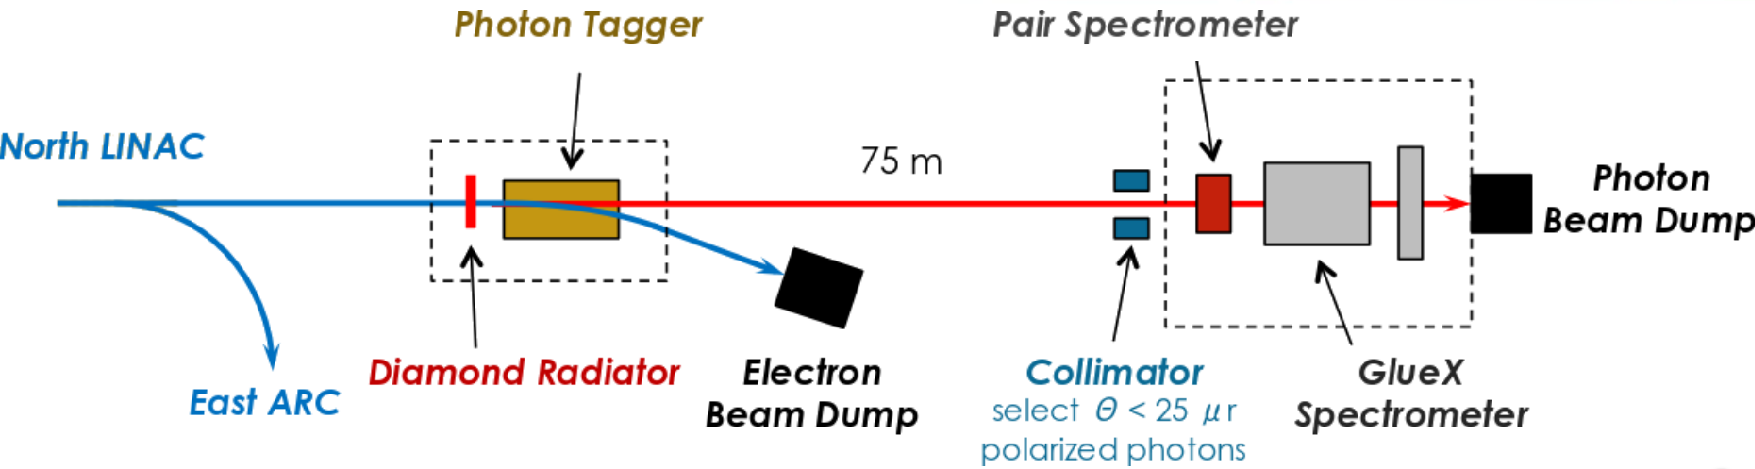
\includegraphics[clip=true,width=0.98\linewidth]{figures/gx_beamline_0}
 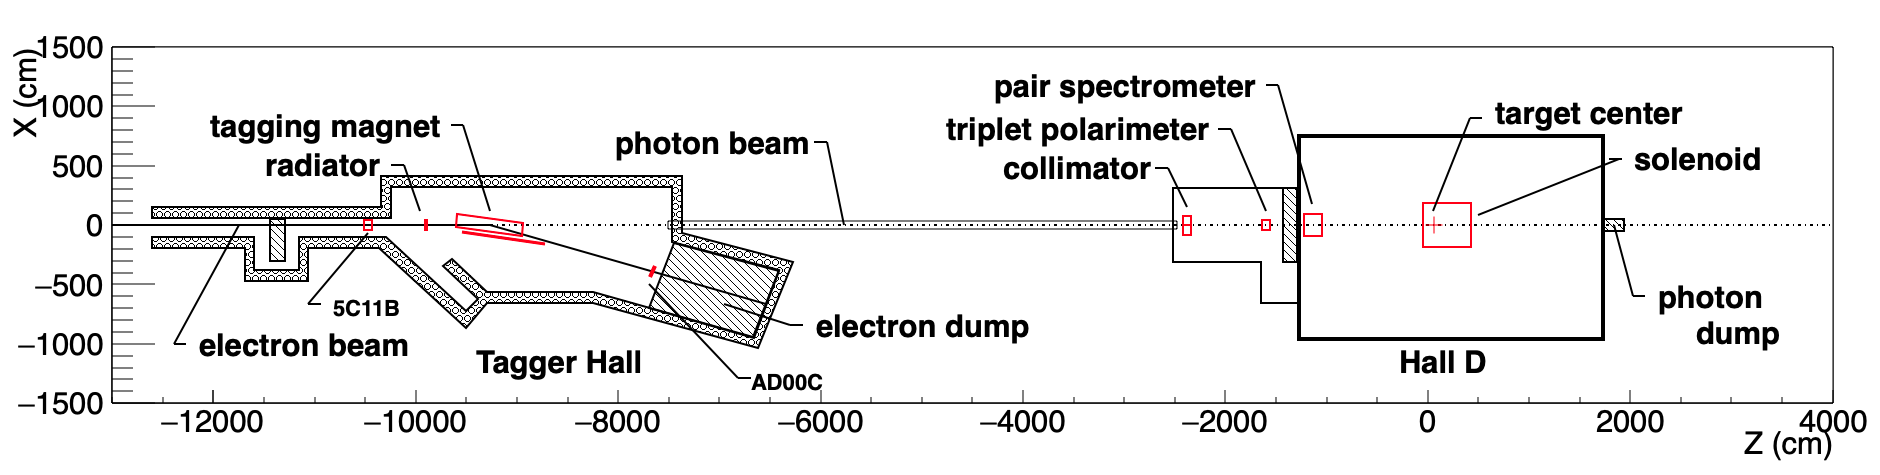
\includegraphics[clip=true,width=0.98\linewidth]{figures/Draw_beamline.png}
\end{center}
\caption{Schematic layout of the Hall D complex, showing the Tagger Hall, Hall D, and several of the key beamline devices. Also indicated are the locations of the 5C11B and AD00 beam position monitors.
        }
\label{fig:beam:Draw_beamline} 
\end{figure}

The photon beam is produced in the Tagger Hall, which is described in more detail in Section\,\ref{sec:tag}.
A properly aligned thin diamond crystal radiator produces linearly polarized photons via coherent bremsstrahlung \cite{timm1969,LIVINGSTON2009205} in addition to photons due to incoherent scattering.
The coherent radiation is peaked at certain energies and is linearly polarized, depending on the crystal orientation with respect to the beam.
The degree of linear polarization in the coherent peak is higher at lower peak photon energies.
In order to increase the ratio of the polarized to unpolarized photons, the photon beam is collimated.  In the nominal \GX{} configuration, we produce the main coherent peak
with maximum energy of 9\,GeV and use a 5.0\,mm collimator.\footnote{A 3.4~mm collimator is also available, and has been used for some physics production runs.}
The beam energy spectrum after collimation and the photon flux are measured by the Pair
Spectrometer, located in Hall D. The photon spectrum and its polarization with a 12\,GeV electron beam are shown in Fig.\,\ref{fig:beam:gx3102_pi0etaAsym2016_fig0_beam}.
The expected degree of linear polarization in the energy range of 8.4--9.0~GeV is $\sim$40\% after collimation. 
The beam polarization is directly measured by the triplet polarimeter upstream of the pair spectrometer. The polarization can also be tracked using various physics channels, such as $\rho$ 
production {\color{red}(Stuart: We should have a reference for this technique)}, even if they cannot determine the absolute value of the polarization. 
{\color{red} Comment by Elton: Somewhere we should add a (typical) plot of the measured convergence of the beam onto the collimator. Do we want add a figure with our harp scan? Perhaps here or maybe in a section below.} 

  
\begin{figure}[t]
\begin{center}
 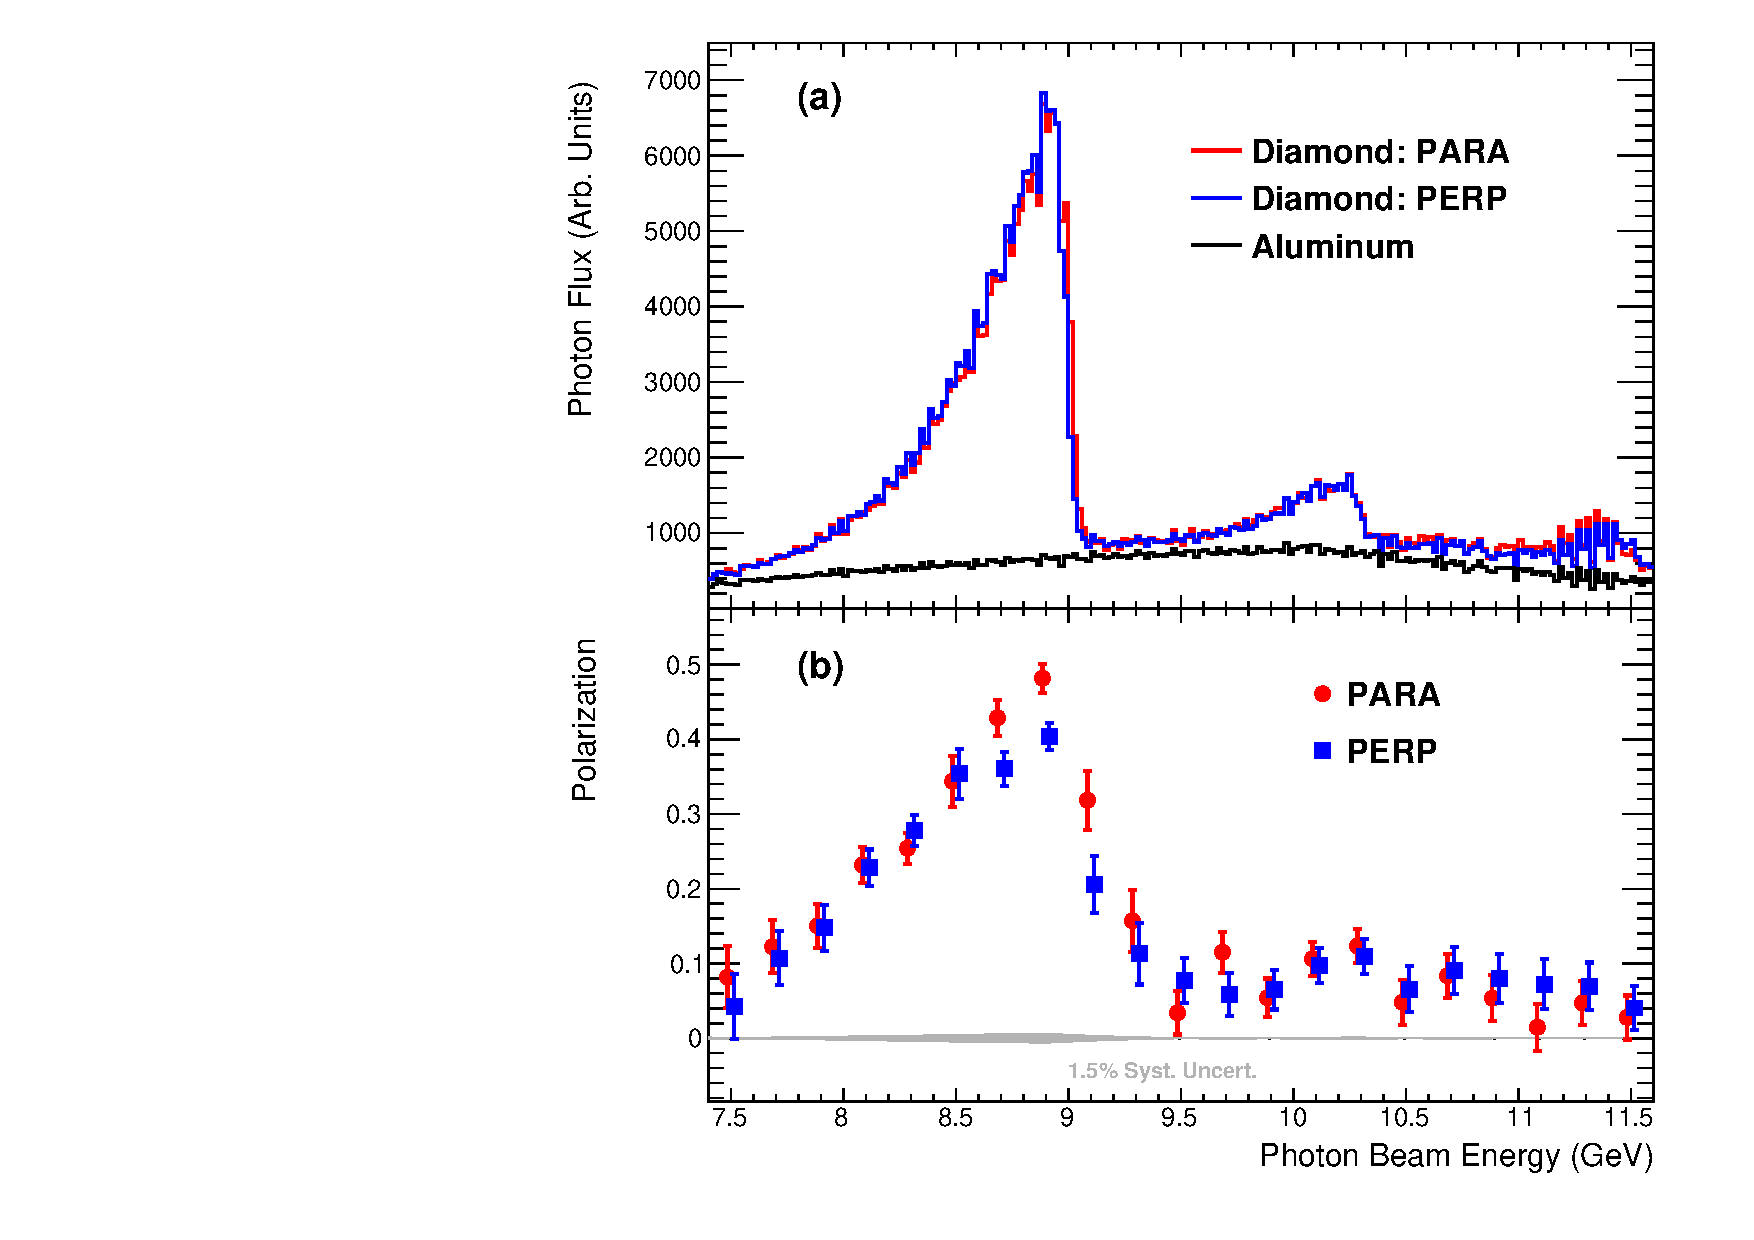
\includegraphics[clip=true,width=0.5\linewidth]{figures/gx3102_pi0etaAsym2016_fig0_beam.pdf}
\end{center}
\caption{(color online) (a) Photon beam intensity versus energy as measured by the pair spectrometer (not corrected for instrumental acceptance).  (b) Photon beam polarization as a function of beam energy, as measured by the triplet polarimeter, with data points offset horizontally by $\pm0.015$~GeV for clarity.
        }
\label{fig:beam:gx3102_pi0etaAsym2016_fig0_beam} 
\end{figure}

In the sections that follow, we describe how the linearly polarized photon beam is produced,  how it is tagged using the tagger spectrometer, how its polarization is determined in the
triplet polarimeter, how the flux is monitored with the pair spectrometer, and how the flux is calibrated using the total absorption counter. The photon is dumped in the photon beam dump
just outside the downstream end of the experimental hall.
The main parameters and properties of the photon beam are given in Table\,\ref{tab:operates}.
  



\begin{table}[tbp]
\begin{center}
\caption[Typical operating parameters for an experiment]{\label{tab:operates}
{\color{red}Note: The values in this table need to be checked!}
Typical operating parameters for an experiment using the coherent bremsstrahlung beam,
calculated with the properties
listed in Table \ref{tab:elecprop}, a diamond radiator of thickness 50~$\mu$m, and the standard
primary collimator of diameter 5.0~mm located at its nominal position.
The electron beam current is taken to 
be $150$~nA. The hadronic rates are calculated for 
a 30~cm liquid hydrogen target.}
%\begin{tabular}{|l|c|c|c|c|}
%\hline\hline
%$E$ upper edge of the peak & 8~GeV & 9~GeV & 10~GeV & 11~GeV \\
%Peak FWHM & 1140~MeV & 900~MeV & 600~MeV & 240~MeV \\
%$N_{\gamma}$ in the peak & 185~MHz & 100~MHz & 45~MHz & 15~MHz \\
%polarization in the peak & 0.54 & 0.41 & 0.27 & 0.11 \\
%%\multicolumn{1}{c}{(F.W.H.M.)} & (1140 \Meunit) & (900 \Meunit) & (600 \Meunit) & (240 \Meunit) \\
%%(F.W.H.M.) & (1140) & (900 \Meunit) & (600 \Meunit) & (240 \Meunit) \\
%peak tagging efficiency & 0.55 & 0.50 & 0.45 & 0.29 \\
%%\multicolumn{1}{c}{(F.W.H.M.)} & (720 \Meunit) & (600 \Meunit) & (420 \Meunit) & (300 \Meunit) \\
%(F.W.H.M.) & (720 \Meunit) & (600 \Meunit) & (420 \Meunit) & (300 \Meunit) \\
%power on collimator & 5.3 W & 4.7 W & 4.2 W & 3.8 W \\
%power on target & 810 mW & 690 mW & 600 mW & 540 mW \\
%total hadronic rate & 385 kHz & 365 kHz & 350 kHz & 345 kHz \\
%tagged hadronic rate & 26 kHz & 14 kHz & 6.3 kHz & 2.1 kHz \\

% The number I entered came from the Bremstrahlung calculator, sometimes estimating averages from the plots
% Power and rates were taken from original table and reduced by a factor of 5.  ES 10/9/2019
\begin{tabular}{|l|r|}
\hline\hline
$E$ upper edge of the peak & 9~GeV \\
Peak effective range       & 8.4 - 9.0~GeV\\
Tagger rate in the peak range & 43~MHz  \\
$N_{\gamma}$ in the peak range after collimator & 24~MHz  \\
Maximum polarization in the peak, after collimator & 40\% \\
Mean polarization in the peak range, after collimator & 35\% \\
Power on collimator & 0.9~W \\
Power on target & 0.14~W \\
Total hadronic rate & 70 kHz \\
Hadronic rate in the peak range & 3 kHz \\
\hline\hline
\end{tabular}
\end{center}
\end{table}


\subsection{Goniometer and Radiators \label{sec:radiators}}
The goniometer\footnote{Manufactured by Newport Corporation} is a device which can position and precisely move horizontally, vertically and rotationally about the x, y and z axes.
The Hall D goniometer holds several radiators, each used depending on the requirements of the experiment.

For the linearly polarized photon beams typically used in \GX{} production running, diamond radiators, typically 50 $\mu m$ thick, are used in the coherent bremsstrahlung technique.
This technique requires precise alignment of a diamond radiator, in order to produce a highly polarized beam by scattering off the appropriate crystal planes associated with a particular reciprocal lattice vector.

Several thin aluminium radiators, of varying thickness, are also available for collecting data to normalise the incoherent bremsstrahlung component from the linearly polarized beam data.

\subsection{Diamond Selection and Quality Control \label{sec:diamonds}}
The properties of diamond make it suitable for use as the radiator in coherent bremsstrahlung; its small lattice constant and high Debye temperature result in small thermal motion of the atoms in the lattice, and its lattice structure suffers minimal thermal effects.

Important considerations when choosing a diamond radiator are its thickness and its purity. The thickness of the radiator affects the angular divergence of the resulting photon beam, due to multiple scattering effects of the electron beam., as can impurities, which can cause defects in the crystal lattice structure \cite{YANG2010719,YANG2012}.
Minimising this divergence enhances the coherent bremsstrahlung spectrum, so the diamond used should be as thin as the considerations of manufacturing and positioning of the radiator allow.

{\color{red}Some further notes on diamond selection and performance (Richard?)}

\begin{figure}[ht]
\begin{center}
   \includegraphics[page=4,viewport=581 1311 3020 2340,clip,angle=0,width=0.98\linewidth]{figures/D000000000-4002_RevB}
\end{center}
\caption{Tagger Hall layout
         from D000000000-4002 {\color{red}Replace this with a simpler figure, based on Dan's field mapping analysis, overlaid with counter positions}
        }
\label{fig:beam:tagger-hall} 
\end{figure}


\subsection{Photon Tagging System \label{sec:tag}}
After passing through a radiator, the mixed photon-electron beam produced enters the photon tagging system (``tagger''), where the electrons are swept out of the beamline by a dipole magnet and detected by one of two systems in the tagger focal plane; the broadband hodoscope (TAGH) or the high resolution microscope (TAGM).
See Fig.\,\ref{fig:beam:tagger-hall}.
A permanent, 0.8~T$\cdot$m dipole magnet is located
downstream of the tagger magnet on the photon beam line, preventing
the electron beam from reaching Hall D should the tagger magnet trip.

Both the TAGM and TAGH devices are used to determine the photon beam energy via the relation $E_{\gamma} = E_{0} - E_{e}$, where $E_{0}$ is the primary electron beam energy from CEBAF, before interaction with the radiator, and $E_{e}$ is the energy of the electron determined by its detected position in the focal plane.
Electrons that did not interact with the radiator are swept into the electron beam dump.


\subsubsection{Tagger Magnet \label{sec:tagMagnet}}
The Hall D tagger magnet deflects electrons in the horizontal plane, allowing the bremsstrahlung-produced photons to continue to the experimental hall while having the electrons that produced them deposited in the focal plane detectors.
Electrons that lost a small amount of energy to bremsstrahlung in the
radiator, or did not interact with the radiator, are deflected by 13.4$^\circ$ into the electron beam dump.
Electrons that lost more than 25\% of their initial energy are deflected into the focal plane of the magnet, and are detected in either the TAGM or TAGH.

The Hall D tagger magnet is a dipole magnet 1.13 m wide, 1.41 m high and 6.3 m long, weighing 80 metric tons.
It has a normal operating field of 1.5 Tesla, with a maximum field of 1.75 T, and a pole gap of 30 mm.
{\color{red} Comments by Elton: Need description of field. Summary of mapping. Uncertainty on absolute field? Uniformity? Standard operation and experience.}


\subsubsection{Tagger Microscope (TAGM)}\label{sec:TAGM}
The Tagger Microscope is a high-resolution hodoscope that counts post-bremsstrahlung electrons corresponding to the photon energy band of interest to the experiment in Hall D.
For a 12 GeV incident electron beam, the microscope is used to tag photons between 8.4 and 9.0 GeV.
This energy changes depending on the primary electron beam energy, and the device is also designed to be movable to center on other energy ranges as demanded by experiment.

Scintillating fibre bundles are oriented towards the incoming electron axis in the tagger focal plane (Fig.~\ref{fig:TAGM_conceptual}), and read out by silicon photomultipliers (SiPMs) at the other end.
This detector provides fine segmentation along the direction of electrons' spread, increasing the energy resolution, as well as allowing selective readout to match the photon collimator acceptance through segmentation in the y-direction.

The TAGM comprises a total of 510, 2$\times$2$\times$20 mm$^3$, multi-clad Saint-Gobain BCF-20 fibers, arranged into 17 bundles of 30 fibers, with each bundle having a 5 row $\times$ 6 column formation. These bundles are spliced to BCF-98 clear fiber light guides, read out by Hamamatsu SiPMs\footnote{Model S10931-050P} mounted on a custom built preamplifier board.
{\color{red} Comments by Elton/Stuart: Further description the system: short description of electronics, energy granularity, energy resolution (e.g. relative to PS), timing resolution, rate capability, summary of operational experience (size of signals in detector, etc.}

\begin{figure}[ht]
\begin{center}
 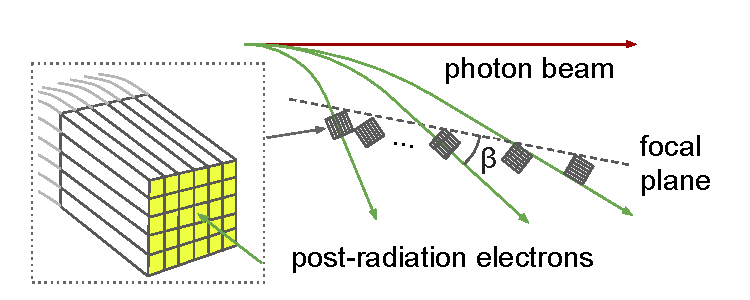
\includegraphics[clip=true,width=0.8\linewidth]{figures/TAGM_conceptual.pdf}
\end{center}
\caption{Conceptual overview of the Tagger Microscope design, showing the fiber bundles and light guides (left), and the orientation of these bundles normal to the incoming electron beam direction in the tagger focal plane (right)
        }
\label{fig:TAGM_conceptual} 
\end{figure}

\subsubsection{Broadband Tagging Hodoscope (TAGH)}\label{sec:TAGHIntro}
The Tagger Hodoscope is a device consisting of $\sim$220 scintillator counters distributed over a length of 9.25 m and mounted just behind the focal plane of the tagger magnet.
Its function is to provide coarse sampling of the full photon energy range from 25\% to 97\% of incident electron energy (3.0 GeV to 11.7 GeV at an electron beam energy of 12 GeV), with a gap in coverage filled by the higher-resolution tagger microscope.
This broad coverage aids in alignment of the diamond radiator and expands the \GX{} physics program reach to photon energies beyond the coherent peak alone.

Each counter in the hodoscope comprises a 6 mm thick and 40 mm high EJ-228 scintillator, of varying widths between 3 and 21 millimetres, coupled to a $\mu$-metal shielded Hamamatsu R9800 PMT via a cylindrical acrylic\footnote{UVT-PMMA} light guide 22.2 mm in diameter and 120 mm long.

The PMTs are instrumented with an active base designed at Jefferson Lab~\cite{tagh:base}. The base consists of a high-voltage divider and an amplifier powered by current flowing through the divider and provides two signal outputs for flash ADC and TDC.
The amplifier with a gain factor of 8.5 allows to operate the PMT at  a smaller voltage of 900 V and reduce the PMT anode current, therefore improving the rate capability. The maximum rate of the counter is about 4 MHz.

The counters are mounted with their faces normal to the path of the scattered electrons, in two rows, either 8 cm or 13 cm from the focal plane.
This allows the counters to be positioned without horizontal gaps in the electron beam direction, enabling complete coverage of the entire tagged photon energy range.

The construction of the hodoscope allows for later addition of counters to fully cover the energy range above the coherent peak for other microscope positions by filling the gaps between sampling scintillators. The mounting frame of the hodoscope is suspended from the Tagger-Hall ceiling to provide full flexibility of microscope positioning.
{\color{red} Comments by Elton: What were typical rates during production running? What is the timing resolution? What is the energy granularity? What is the energy resolution (e.g. compared to PS)?}

\subsection{Beam profiler}
The beam profiler is located immediately upstream of the collimator and is used to measure photon beam profiles.
The profiler consists of two planes of scintillator fibres, giving information on the photon beam profile in the X and Y directions.
Each plane is made up of 64 square fibres, 2 mm in width, read out by eight {\color{red} (Elton: 8 total or 8/side?)} multi-anode PMTs. The profilers are only used during beam setup until
the beam is centered on the active collimator and it can be used reliably to provide feedback on the beam position. They are retracted during physics production runs.
{\color{red} Comments by Elton: Is there a Hall B reference for these detectors?}

\subsection{Active collimator \label{sec:coll}}
The Active Collimator monitors the photon beam position and provides fast feedback to micro-steering magnets in the electron beamline, for the purpose of suppressing drifts in beam position.
It is located in the collimator cave area, on the front face of the primary collimator, and consists of a large tungsten plate, divided into two radial rings and four quadrants. The design of the active collimator is based on a device pioneered at SLAC for monitoring their coherent bremsstrahlung beam \cite{Miller:1973yi}. 
{\color{red} Comments by Elton: Short description of device; reference should help those interested in more details. Need to add position resolution (inner and outer) and stability. Add comment on operational experience with the feedback loop in place.}

When a beam photon interacts with the plates, it creates a particle shower, detected by arrays of tungsten wires mounted parallel to the beam direction on each section of the Active Collimator.
These induce currents in the plate which indicate the degree of displacement of the beam from its intended center position.

\subsection{Collimator}
The photon beam produced at the diamond radiator contains both incoherent and coherent bremsstrahlung components.
In the region of the coherent peak, where photon polarization is at its maximum, the angular spread of coherent bremsstrahlung photons is less than that of incoherent bremsstrahlung.
The coherent radiation is concentrated at small angles $<$25~$\mu$rad with respect to the beam direction, while the incoherent radiation has a broader angular distribution.
To maximise the degree of linear polarization in the photon beam, it is tightly collimated.

The Hall D primary collimator provides apertures of 3.4 mm and 5.0 mm in a tungsten plate mounted on an X-Y table, the latter of which is typically used in normal \GX{} running conditions.
The entire collimator is surrounded by lead shielding.
The device may also be positioned to block the beam to prevent high current beam, occasionally delivered by CEBAF for the purposes of beam tuning, from entering the experimental hall. Following this primary collimator, there is a sweeping magnet and a secondary cleanup collimator, magnet and 
lead shielding to remove unwanted charged particles from the photon beam. The photon beam exiting the collimation system is delivered to the systems downstream for monitoring and use in physics experiments.

\subsection{Triplet polarimeter \label{sec:tpol}}
The triplet polarimeter, or TPol, is used to measure the degree of polarization of the linearly polarized photon beam \cite{DUGGER2017115}.
The polarimeter uses the process of pair production on atomic electrons in a beryllium target foil, with these scattered atomic electrons measured using a silicon strip detector.
Information of the degree of polarization of the photon beam can be obtained by analysing the azimuthal distribution of the scattered atomic electrons measured by this device.
{\color{red} Comments by Elton: Useful to add a little information on how data are taken and how much statistics is needed to determine the polarization}.

\subsection{Pair spectrometer         (Sasha) \label{sec:ps}}

The Pair Spectrometer \cite{BARBOSA2015376} is located at the entrance to Hall D.
%(Fig.~\ref{fig:beam:hall-d}).
The spectrometer reconstructs the energy of a beam photon by detecting the $e^\pm$ pair produced by the photon in a thin converter. 
Electrons and positrons are registered in two layers of scintillator
detectors: a high-granularity hodoscope and a set of coarse counters,
referred to as PS and PSC, respectively. The detectors are organized into two arms positioned symmetrically with respect to the photon beam line. The PSC consists of sixteen scintillator counters, eight in each detector arm. Each counter is 4.4 cm wide, 2 cm thick in the direction along the lepton trajectory and 6 cm heigh. The pair spectrometer hodoscope consists of 145 rectangular 
tiles (1 mm and 2 mm wide) stacked together. Light from the PSC counters is detected using Hamamatsu R6427-01 PMTs. Hamamatsu silicon photomultipliers were chosen for the instrumentation of the PS hodoscope~\cite{Barbosa:2017zzw,Somov:2017kif,Tolstukhin:2014zsa}.

Each detector arm covers a momentum range of $e^\pm$ between 3.0 GeV/c and 6.2 GeV/c, 
corresponding to reconstructed photon energies between 6~GeV and 12.4~GeV. The relatively
large acceptance of the hodoscope allows one to reconstruct photons
with energies in the coherent peak energy region and also in the range
near the beam end-point energy of 12~GeV. Some details about the performance of the spectrometer are given in~\cite{Somov:2017vhp,Somov:2016bgb}.

The main purpose of the spectrometer is to measure the spectrum of the
collimated photon beam and determine the fraction of linearly polarized
photons in the coherent peak energy region.
It is also used to monitor the photon beam flux and can be used for 
energy calibration of the tagging hodoscope and microscope detectors.
{\color{red} Comments by Elton: Further description (Can refer back to Fig with photon flux and polarization) What is the timing resolution? Rate of PS triggers? What is the energy resolution? Stability of the system?}


%\subsubsection[Spectrometer]{Spectrometer\label{sec:beamline:ps-spetrometer}}

%Layout of the Hall D pair spectrometer is presented in Fig.~\ref{fig:beam:ps-layout}. 
% --------------------------------------------
%\begin{figure}[h]
%\begin{center}
%%   \tikzstyle{background grid}=[draw, black!50,step=.5cm]
%%   \begin{tikzpicture}[show background grid]
%%%   \begin{tikzpicture}[]
%%                  % The above right option is used to place the lower left corner
%%                  % of the image at the (0,0) coordinate. 
%%     \node [inner sep=0pt,above right] 
%%      {\includegraphics[angle=0,width=0.98\linewidth]{figs/ps_layout}};
%%       \node (halla)    at (2.0,0.3) [] {{\color{yellow} \scalebox{1.0}{\large A}}};  
%%       \draw[->,yellow,very thick] (halla) edge [] (3.25,1.75);
%%   \end{tikzpicture}
%   \includegraphics[angle=0,width=0.98\linewidth]{figs/ps_layout}
%\end{center}
%\caption{Pair Spectrometer simplified layout. In reality the detectors 
%         are tilted by 4.7$^\circ$ - perpendicular to the average trajectories.}
%\label{fig:beam:ps-layout} 
%\end{figure}
% --------------------------------------------

%Electron-positron pairs are created by beam photons inside a thin
%converter with a typical thickness ranging between 0.03\% and 0.5\% of
%a radiation length. The choice of the converter thickness depends on
%the photon beam flux. The maximum photon flux for GlueX physics runs
%is expected to be 50~MHz in the coherent peak energy region. Three
%converters with different thicknesses are installed in a movable fork
%that can insert one of them into the photon beam. Produced leptons are
%deflected in a 18D36 dipole magnet with an effective field length of
%about 0.94~m. The magnet was brought from Brookhaven National
%Laboratory and was modified at Jefferson Lab by reducing the pole gap
%from 6 inches to 3 inches. The magnet is operated at a nominal field
%of 1.8~T; the field integral is $\int{}Bdl\approx$1.60~T\,m. The beam
%angular spread is $<0.04$~mrad, and the angular spread of the pair
%production is $\sim{}\gamma^{-1}<0.2$~mrad. The multiple scattering at
%3~GeV in the thickest converter adds about 0.3~mrad. The particle
%deflection by the magnet at the momentum $p$ is
%$\theta{}=0.3\,[\mathrm{GeV/c/T/m}]\int{}Bdl/p$;
%$\theta\approx{}80~\mathrm{mrad}=4.6^\circ$ at 6~GeV.  
%A 1.5~m long vacuum chamber is installed after the magnet.
%Electrons and positrons are registered in two layers of scintillator detectors: a
%high-granularity hodoscope and a set of coarse counters, referred to as PS and PSC, respectively.
%The detectors are organized into two arms positioned symmetrically with
%respect to the photon beam line.  Each detector arm covers a momentum
%range of $e^\pm$ between 3.0 GeV/c and 6.2 GeV/c, corresponding to
%reconstructed photon energies between 6~GeV and 12.4~GeV. Relatively
%large acceptance of the hodoscope allows one to reconstruct photons
%with energies in the coherent peak energy region and also in the range
%near the beam end-point energy of 12~GeV. This can be used for the
%energy calibration of the hodoscope detectors.

%\begin{table}[h]
%  \begin{center}
%    \caption{The coordinates of the inner counters (the edge closest to the beam)
%             with respect to the magnet center. The survey was done at 2-Nov-2015. 
%       \label{tab:beam:ps-ccordinates}
%    }
%    %\vspace{3mm}
%    \begin{tabular}{l|r|r}
%       \hline
%       Detector & $Z$, mm & $X$, mm \\
%       \hline
%       \hline
%       PS~ Right arm & 2928.4 & -238.7 \\
%       PS~ Left~ arm & 2928.3 &  238.3 \\
%       PSC Right arm & 3416.2 & -274.4 \\
%       PSC Left~ arm & 3416.1 & ~274.8 \\
%       \hline
%    \end{tabular}
%  \end{center}
%\end{table}

%\subsubsection[PS: High Resolution Detector]{PS: High Resolution Detector
%  \label{sec:beamline:ps-hresol}
%}
%
%Each arm of the high resolution detector consists of 145 rectangular
%tiles made of EJ-212 scintillator~\footnote{
%  ELJEN Technology Plastic Scintillators \url{http://www.eljentechnology.com}. 
%}, stacked together as
%shown in Fig.~\ref{fig:beam:ps-tiles}. The tile height is 3 cm and the
%length along the particle path in scintillator is 1 cm. Out of 145 tiles,
%40 tiles close to the beam are 1~mm thick, the rest are 2~mm thick.
% The momentum bin size of the tile depends on the electron/positron energy as 
%%$\Delta{}p=\Delta{}x/x\cdot{}p$ 
%and constitutes about 13~MeV/c for 3~GeV and 24~MeV/c for 6~GeV particles.
%Tiles are optically isolated using 10~$\mu$m
%aluminized Mylar foil. This reflective foil also covers the bottom of
%the tile assembly. In order to keep the tiles parallel to the
%particle trajectories, the tiles are organized into 18 groups. Each
%group is tilted by $\sim$0.005~mrad using 0.05~mm thick shims
%(adhesive strips) positioned between the adjacent groups. The 
%first group is tilted by about 80~mrad, so that the tiles are parallel
%the 6~GeV particle trajectories.
%
%Light from a tile is collected using two 20~cm long 2$\times$2~mm$^2$
%double-clad BCF-92 wave-length shifting (WLS) fibers,
%glued to the sides of the tile using BC 600 Optical Cement. A tile
%assembly with two WLS optical fibers is shown in
%Fig.~\ref{fig:beam:ps-tiles}. The peak of the emission spectrum for EJ-212
%%scintillator occurs at the wavelength of 423 nm, which couples well
%with the absorption spectrum of the BCF-92 fiber. Light is
%subsequently re-emitted inside the fiber in the green range with an
%emission peak of 492 nm.
%
%Collected light is transmitted to the end of the WLS fiber. A pair of
%fibers from each tile is inserted into a hole in an aluminum mounting
%plate. %, as shown on the upper plot of Fig.~\ref{fig:hodoscope}. 
%The light detection is performed using Hamamatsu
%surface mount S10931-050P silicon photomultipliers with an effective
%photosensitive area of 3$\times$3~mm$^2$ and a pixel size of 0.05$\times$0.05~mm$^2$.
%These sensors have a photon detection efficiency (PDE) larger
%than 20\% at a wavelength of 500~nm and a typical gain of about
%$7\cdot{}10^5$~\footnote{
% Hamamatsu Corporation, MPPC S10931-050P, 
% \url{http://www.electronicsdatasheets.com/pdf-datasheets/hamamatsu/s10931050p}.
%}.
%Each photo sensor is coupled to two WLS fibers
%from a single tile.
%The electronics board (Fig.~\ref{fig:beam:ps-electr-assemb} left) 
%with 145 SiPMs is attached
%to the mounting plate.
%The SiPMs are arranged in two arrays
%of 3$\times$35 and 5$\times$8 sensors, which are connected to 2~mm and~1 mm
%tiles, respectively. SiPMs are optically isolated using a plastic
%spacer.
%
%
%% --------------------------------------------
%\begin{figure}[h]
%\begin{center}
%   \includegraphics[angle=0,width=0.45\linewidth]{figs/ps_tiles_photo_small}\hspace{0.05\linewidth}%
%   \includegraphics[angle=0,width=0.38\linewidth]{figs/ps_assembly_photo}
%\end{center}
%\caption{Scintillator tiles with two WLS fibers glued to sides of each tile: %30$\times$10$\times$1~mm$^3$ tile (left) 
%         and 30$\times$10$\times$2~mm$^3$  tile (right).
%        }
%\label{fig:beam:ps-tiles} 
%\end{figure}
%% --------------------------------------------
%
%% --------------------------------------------
%\begin{figure}[h]
%\begin{center}
%   \includegraphics[angle=0,width=0.43\linewidth]{figs/ps_sipm_plate_photo}\hspace{0.05\linewidth}%
%   \includegraphics[angle=0,width=0.47\linewidth]{figs/ps_assembly_drawing}
%\end{center}
%\caption{Electronics board with 145 SiPMs (left); 
%         the PS detector assembly (right).
%        }
%\label{fig:beam:ps-electr-assemb} 
%\end{figure}
%% --------------------------------------------

%\subsubsection[PSC: Coarse Resolution Detector]{PSC: Coarse Resolution Detector
%  \label{sec:beamline:ps-coarse} }
%
%Sixteen coarse scintillator counters, eight in each detector arm, are
%positioned about 40~cm behind the hodoscope.  The counters are 4.4~cm
%wide in the direction perpendicular to the particle trajectory, 2~cm
%thick, and 6~cm in height.  Hamamatsu R6427-01 PMTs are used to detect
%the scintillation light. The counters are used to produce a pair
%spectrometer trigger by requiring a coincidence of hits in the two
%detector arms. They also help to reduce background originating from
%interactions of $e^\pm$ inside the magnet pole edges to the level
%below 1\% by constraining the $e^\pm$ trajectories.  Counter rates
%depend on the converter thickness and photon beam flux. The maximum
%rate will not exceed 10~kHz per PSC counter during GlueX operation.
%
%
%\subsubsection[Electronics]{Electronics\label{sec:beamline:ps-electronics}}
%
%The PS hodoscope front end electronics consists of an amplifier and a
%SiPM bias voltage control circuit developed at Jefferson Lab. Signals
%from the SiPMs are amplified using the amplifier with a gain of about
%a factor of 20.  The amplifier is based on commercially available
%devices (operational amplifiers) with 3~GHz bandwidth.  Pulse shaping
%is employed to compensate for the characteristically high SiPM
%capacitance and package inductance. The impulse response shows rise
%and fall times of 3~ns and with trans-impedance gain of 1~mV/$\mu$A.  
%The SiPM operating bias voltage is about 73~V. The
%nominal bias setting is as specified by Hamamatsu (1~V over voltage)
%and fed to the SiPM through a resistive network employing a thermistor
%and a linearizing resistor. The hodoscope control electronics supply
%individually adjusted voltages to groups of 5 SiPM channels; inside
%the group the voltage is adjusted among channels using resistors. The
%thermistor senses the average temperature of closely packed SiPMs in
%thermal equilibrium via a heat spreader PCB layout, thus forming a
%well controlled loop. 
%%The commercially available bias power supply has
%%very low noise characteristics and is well regulated to less than 1~mV
%%long term. The supply allows the user to monitor and adjust the levels
%%as needed and if required. The optimal bias setting will be determined
%%based on experimental conditions.
%
%Signals from both the hodoscope and coarse counters are digitized
%using a twelve-bit multi-channel flash ADC operated at a sampling rate
%of 250~MHz (fADC250-MHz). The PSC counters are also instrumented with
%TDCs, with the intrinsic resolution of $\sim$60~ps.  The timing resolution
%is expected to be better than 200~ps. 
%
%An example of the fADC signal pulse obtained from a PS scintillator
%tile is shown in Fig.~\ref{fig:beam:ps-signals} (left).  The ADC
%sampling time is 4~ns. The SiPMs allow to resolve the number of pixels
%fired, demonstrated in Fig.~\ref{fig:beam:ps-signals} (right). The
%average amplitudes of the signals in the Pair Spectrometer correspond
%to about 60 pixels fired.
%
%%This resolution will allow one
%%to distinguish the electron beam bunch where the bremsstrahlung photon
%%is emitted and therefore relate hits from the pair spectrometer and
%%tagging detectors originating from the same event.
%
%% --------------------------------------------
%\begin{figure}[h]
%\begin{center}
%   \includegraphics[angle=0,width=0.45\linewidth]{figs/ps_sipm_pulse}\hspace{0.05\linewidth}%
%   \includegraphics[angle=0,width=0.45\linewidth]{figs/ps_sipm_pixels_peaks}
%\end{center}
%\caption{PS typical fADC250-MHz signal (left); 
%         PS The spectrum of fADC signals integrated in 60~ns, obtained using a low intensity light source. 
%         The spectrum
%         resolves the peaks from different numbers of pixels fired,
%         including zero (the pedestal) (right).
%        }
%\label{fig:beam:ps-signals} 
%\end{figure}


\subsection{Total absorption counter \label{sec:tac}}
The Total Absorption Counter (TAC) is a high-efficiency lead glass calorimeter, used at low beam currents ($<5$nA) to determine the overall efficiency of the coherent bremsstrahlung facility.
The TAC was originally developed for and deployed in Hall B, for real photon beam operations with CLAS \cite{clasnote1992014, clasnote1993011, clasnote1999002}, and was transferred to Hall D to serve the same purpose for \GX{}.
Not every photon produced at the radiator reaches the hall, and in normal \GX{} running not every photon that reaches the hall causes an interaction that is seen in the \GX{} detector.

Using the TAC at normal \GX{} production currents is not possible, as it would very quickly succumb to radiation damage, therefore the TAC is used to measure photons reaching it at low currents with near 100\% efficiency.
From this measurement, the fraction of bremsstrahlung produced photons reaching \GX{} at nominal operational beam currents can be determined by extrapolation.
{\color{red} Comments by Elton: Describe how the PS measures the relative rate and the TAC is used to determine the absolute flux assuming the PS is a linear device.}

{\color{red} Comment by Stuart: TAC runs have also been performed using v-wires during GlueX phase I, and the CompCal (although the latter may count as PrimEx commissioning). Should we mention either of these?}

Finally, the photon beam travels through the \GX{} detector, and
ultimately goes to the photon beam dump just outside the downstream
end of the experimental hall.
The main parameters and properties of the Photon Beam are given in and \ref{tab:operates}.
{\color{red} Comment by Stuart: Hasn't this already been stated at the beginning of this section?}



\subsection{Flux normalization \label{sec:fluxnorm}}
(Status 09/30/2019: Materials collated, section will be included after collaboration meeting)

\subsection{Photon polarization (M. Dugger/ASU Student)\label{sec:polarization}}
%=======================+=========================
%================   Solenoid  ================
%=================================================

\section[Solenoid Magnet]{Solenoid magnet 
  \label{sec:solenoid}
}

\subsection[Overview]{Overview \label{sec:sol:overview}
}

The core of the GlueX spectrometer is a superconducting magnetic
solenoid with a bore of about 2~m in diameter and the overall
yoke's length of about 4.8~m. The photon beam passes along the axis of
the solenoid.  At the nominal current of 1350~A used for the GlueX
experiment the magnet provides a $\approx$2~T field at its axis.

The magnet was designed and built at SLAC in the early
1970's~\cite{Alcorn-confer-1972} for the LASS
spectrometer~\cite{Aston:1987uc}. It is a cryostatically
stable design and uses cryostats that were designed to be opened and
serviced with hand tools. It was refurbished and modified%
\footnote{
  The front plate of the flux return yoke was modified, leading to a
  swap of the two front coils and modifications of the return flux
  yoke in order to keep the magnetic forces on the front coil under
  the design limit.  The original gaps between the yoke's rings were
  filled with iron. The Cryogenic Distribution Box was designed and
  built anew.
} 
for the GlueX experiment~\cite{Ballard:2011tm, Ballard:2015wma}. 

The magnet is constructed of four separate superconducting coils and
cryostats. The flux return yoke is made of several iron rings.  The
coils are connected in series. A common liquid helium tank is located
atop the magnet providing the gravity feed of the liquid to the
coils. The layout of the coils' cryostats and the flux return iron
yoke is shown in Fig.~\ref{fig:layout_spectrometer}.
Table~\ref{tab:sol:summary} summarizes the important magnet
parameters.

% ======================================================================================
  

\begin{table}[h]
 \begin{center}
   \small
   \begin{tabular}{lr}
     \hline
     \hline
       Inside diameter of coils        & 2032 mm \\
       Clear bore diameter             & 1854 mm \\
       Overall length along iron       & 4795~mm \\
       Inside iron diameter            & 2946~mm \\
       Outside iron diameter           & 3759~mm \\
       Original yoke, cast and annealed - steel & AISI 1010 \\
       Added filler plates - steel     & ASTM A36 \\
       Full weight                     & 284~t      \\
       Full number of turns            & 4608 \\
       Number of separate coils        & 4 \\
%       Longitudinal arrangement of coils & 1-2-3-4 & & 2-1-3-4 \\
       Turns per coil 2                &  928 \\   
       Turns per coil 1                & 1428 \\   
       Turns per coil 3                &  776 \\   
       Turns per coil 4                & 1476 \\   
       Total conductor weight          & 13.15 t \\
       Coil resistance at $\sim$300~K & 15.3~$\Omega$ \\   
       Coil resistance at  $\sim$10~K & $\sim$0.15$\Omega$ \\   
       Design operational current      & 1500 A \\
       Nominal current (actual)        & 1350 A \\
       Maximal central field at 1350~A & 2.08 T \\   
       Inductance at 1350~A            & 26.4 H \\
       Stored energy at 1350~A         & 24.1 MJ  \\
       Protection circuit resistor     & 0.061 $\Omega$  \\
%       Total conductor length        & 117600 ft & 35.84 km & {\it same} \\
%       Substrate material            & \multicolumn{1}{r}{Copper} & & {\it same} \\   
%       Copper-to-filament ratio (A)  & \multicolumn{1}{r}{20:1} & & {\it same} \\   
%       Copper-to-filament ratio (B)  & \multicolumn{1}{r}{28:1} & & {\it same} \\   
       Coil cooling scheme             & helium bath \\   
       Total liquid helium volume      & 3200 $\ell$ \\
       Operating temperature (actual)  &  4.5~K \\   
       Refrigerator liquefaction rate at 0~A        & 1.7~g/s    \\
       Refrigerator liquefaction rate at 1350~A     & 2.7~g/s    \\
%       Refrigerator liquefaction rate at 0~A        & 1.7~g\thinspace{}s$^{-1}$    \\
%       Refrigerator liquefaction rate at 1350~A     & 2.7~g\thinspace{}s$^{-1}$    \\
%       Protection circuit limiting voltage & 500 V & & 90 V \\
     \hline
   \end{tabular}
   \normalsize
 \end{center}
  \caption{
    The actual parameters of the solenoid.  The units are metric. The
    coils are ordered along the beam direction.
    \label{tab:sol:summary}
  }
\end{table}


\subsection[Conductor and Coils]{Conductor and Coils
 \label{sec:sol:coils}
}

The superconductor composite is made of niobium--titanium filaments
%\footnote{The critical temperature is about 10$^\circ$K.} 
in a copper substrate, twisted and shaped into a
$\sim$7.62$\times$1~mm$^2$ rectangular band. The laminated conductor
is made by soldering the superconductor composite band between two
copper strips
%\footnote{Copper CDA 102. Average Resistivity Ratio for
%  300$^\circ$K:4.2$^\circ$K is a minimum of 150:1, claimed by the builders of the
%  magnet\cite{Solen-conductor}. 
%  %It contradicts the data from another
%  %source\cite{CuHandbook}, which specifies $10<$RRR$<100$ for ETP
%  %copper. 
%  Our measurements show RRR$\approx{}$100.
%} 
to form a rectangular cross section of 7.62$\times$5.33~mm$^2$
%\cite{Alcorn-confer-1972}.  
The measured resistivity ratio of the conductor at $\sim{}300^\circ{}$K and
$\sim{}15^\circ{}$K is $\approx{}$100.  
%Two types of filaments have
%been used (see Fig.~\ref{fig:sol:conductor-cartoon} and
%Table.~\ref{tab:sol:conductor}). The Grade A conductor provides a higher
%current limit than the Grade B conductor and is used in the area of
%the highest magnetic field (Coil 4).

%The coil was wound on G-10 standoff strips glued on the cylindrical
%inner wall of the liquid helium vessel.  
As the coil was wound, a 0.64~mm-thick stainless steel support band
and two 0.2~mm-thick Mylar insulating strips were wound along with it
for pre-tensioning and insulation%
%(Fig.~\ref{fig:sol:conductor-cartoon})
. 
The liquid helium is in contact with the shorter (5.33~mm) sides of
the cable.

Each of the coils consists of a number of subcoils. Each subcoil
contains a number of ``double pancakes'' with the same number of
turns.
%(see Table~\ref{tab:sol:coils-turns}). 
Each double pancake is made from a single piece of conductor. The
voltage across the subcoils is monitored using special wires passing
through the coils' chimneys along with the helium supply pipes and the
main conductor.

The cold helium vessel containing the coil is supported within its
warm cryostat vacuum vessel by a set of columns designed to provide
sufficient thermal insulation. The columns are equipped with strain
gauges for monitoring the stresses on the columns. The helium vessel
is surrounded by a nitrogen-cooled shield made of copper panels.
Super-insulation is placed between the vacuum vessel and the nitrogen
shield.  The vacuum vessels are attached to the matching iron rings of
the yoke.

The power supply%
\footnote{Danfysik System 8000 Type 854.}
provides up to 10~V DC for ramping up/down the current. It also
includes a protection circuit, which can be fired by the quench
detector as well as by other signals.  A relatively low dump resistor
of 0.061~$\Omega$ limits the maximal voltage on the magnet during
trips to 100~V. The dumping time constant of $L/R \approx 7$~min is
relatively long, but safe according to the original design of the
magnet. A large copper mass and the helium bath are able to absorb a
large amount of energy during a quench without overheating the solder
joints. This allowed for a relatively slow-reacting - 0.5~s decision
time - but more noise-proof and ``intelligent'' quench detector.  The
quench detector compares the measured voltages on different subcoils
in order to detect a resistive component that might appear in a
subcoil.
%The decision is made based on the measured voltages on the
%subcoils.  
During ramping the current up or down such a voltage is proportional
to the subcoil's inductance.  Relative values of inductance of various
subcoils depend on the value of the current because of saturation
effects in the iron yoke. There are also transient effects at changes
of the slew rate caused by Foucault currents in the yoke.
%The quench detector compares
%voltages on different subcoils in order to detect a resistive
%component that might appear in a subcoil.  
The system includes two redundant detectors - one uses analog signals
and a simplified logic, another is done in the PLC control system (see
Section~\ref{sec:sol:controls}) which uses digitized signals. The PLC
digital programmable device is more sensitive since it takes into
account the dependence of the coils' inductance on the current and
provides a better filtering of the noise.  The ramping slew rate is
limited by the transient imbalance of the voltages on subcoils, that
may trigger the quench detector. Additionally, $\sim$1~ms-long voltage
spikes of unidentified origin have been observed in coil 2 at high
slew rates, also triggering the quench detector. Powering up the
magnet to 1350~A takes about 8~h.

For diagnostic purposes two 40-turns pickup coils are installed on the bore
surface of the vacuum vessel of each of the coils. 

\subsection[Cooling System]{
   Cooling System
   \label{sec:sol:cryo}
}

The cooling system is described in detail in Ref.~\cite{Lavendure:2014:refrig}.
A standalone helium refrigerator located
in a building adjacent to Hall D provides liquid helium and nitrogen
via a transfer line to the Cryogenic Distribution Box atop the
magnet. The transfer line delivers helium at 2.6~atm and 5~K to a Joule-Thomson
(JT) valve providing liquid to a cylindrical common helium tank in the
Distribution Box. The level of liquid helium in the tank is measured
with a superconducting wire probe%
\footnote{
  American Magnetics Model 1700 with HS-1/4-RGD-19"/46"-4LDCP-LL6-S sensor
}
 and is kept at about half of the tank's diameter. The cold helium gas
 from the tank is returned to the refrigerator which keeps the
 pressure at the top of the tank at 1.2~atm corresponding to about
 4.35~K at the surface of the liquid%
\footnote{
  The original implementation at SLAC did not recycle the helium and
  operated at atmospheric pressure.
}
.
Each coil is connected to the common helium tank by two vertical 2-inch
pipes.  One pipe is open at the bottom of the tank while the other one
is taller than the typical level of helium inside the tank. The main
conductor and the wires for voltage monitoring pass through the former
pipe. Additionally, two $\sim$6~m long, 3/8~inch ID pipes go outside
the coil's helium vessel, from the Distribution Box to the bottom of
the coil. One of those pipes is connected to a JT valve in the Box,
and is used to fill the coil initially and is not used during operations.
Another one reaches the bottom of
the common helium tank in order to provide 
a thermosyphon effect essential
for the proper circulation of helium in the coil. The main current is
delivered into the helium tank via vapor-cooled leads and is
distributed to the coils by a superconducting cable. After cooling the
leads the helium gas is warmed up and returned to the refrigeration
system. The gas flow through the leads is regulated depending on the
current in the magnet and at 1350~A the flow is about 0.25~g/s. The
coils and the Distribution Box are equipped with various sensors for
temperature, pressure, voltage, and flow rates.

\subsection[Measurements and Controls]{
         Measurements and Controls
        \label{sec:sol:controls}
}

The control system for the superconducting solenoid, the power supply, 
and the cryogenic system, is based on Programmable Logic
Controllers (PLC)%
\footnote{
  Allen-Bradley Programmable Logic Controllers
  \url{http://ab.rockwellautomation.com/Programmable-Controllers}.
}%
.
The PLC digitizes the signals from various sensors, communicates with
other devices, reads out the data into a programmable unit for
analysis, and sends commands to various devices. Additionally, it is
connected to EPICS in order to display and archive the data (see
Section \ref{sec:controls}).  The practical sampling rate of a
sensor's readout is limited to a few Hz, which is too low for
detection of fast voltage spikes on the coils due to motion, shorts,
or other effects. Therefore, the voltage taps from the coils
and the pickup coils are read
out by a PXI%
\footnote{
  National Instruments, PXI Platform, \url{http://www.ni.com/pxi/}.
}%
system, which provides an initial sampling rate of about 100~kHz. The
PXI system also reads out several accelerometers attached to the
coils' chimneys, which may detect a motion inside the coils. The PXI
CPU performs initial integration and arranges the data in time-wise
rows with a sampling rate of 10~kHz.  The PLC system reads out these
data from the PXI system. Additionally, the PXI data are read out by
an EPICS server at the full 10~kHz sampling rate and are recorded 
to files for further analysis.

\subsection[Field Calculation and Measurement]{
         Field Calculation and Measurement
        \label{sec:sol:field}
}

The momentum resolution of the GlueX spectrometer is larger than
1\% and is dominated by multiple scattering and the spatial
resolution of the coordinate detectors.  A fraction of a percent is a
sufficient accuracy for the field determination.  The coils are
axially symmetric while the flux return yoke is nearly axially
symmetric, apart from the holes for the coil's chimneys. The field was
calculated using a 2-dimensional field calculator {\it
  Poisson/Superfish}%
\footnote{
   Poisson/Superfish developed at LANL,
   \url{https://laacg.lanl.gov/laacg/services/serv_codes.phtml\#ps}.
} 
, assuming axial symmetry.  The model of the magnet included the
fine structure of the subcoils and the geometry of the yoke
iron. Different assumptions about the magnetic properties of the yoke
iron have been used: the {\it Poisson} default AISI 1010 steel, the
measurements of the original yoke iron made at SLAC, and the 1018
steel for the filler plates. Since the results of the field
calculations differ for less than 0.1\% the default {\it Poisson} AISI
1010 steel properties for the whole yoke iron were used for the final
field map calculations.

The 3 projections of the magnetic field have been measured along lines
parallel to the axis, at 4 values of the radius and at up to 6 values
of the azimuthal angle. The calculated field and its deviation from
the measurements are shown in Fig.~\ref{fig:sol:field_comparison}. The
tracking detectors occupy a volume of $R<56$~cm and $45<Z<340$~cm. In
this volume the field deviation at $R=0$ does not exceed 0.2\%. The
largest deviation of 1.5\% is observed at the downstream edge of the
fiducial volume and at the largest radius. Such a field uncertainty in
that region does not affect noticeably the momentum resolution. In
most of the fiducial volume the measured field is axially symmetric to
$\approx$0.1\% and deviates from this symmetry by $\approx$2\% at the
downstream edge and the largest radius.

The calculated field map is being used for the track reconstruction and
physics analysis.
   
% ======================================================================================

%\begin{figure}[tp]
\begin{figure}[!htb]
  \begin{center}
     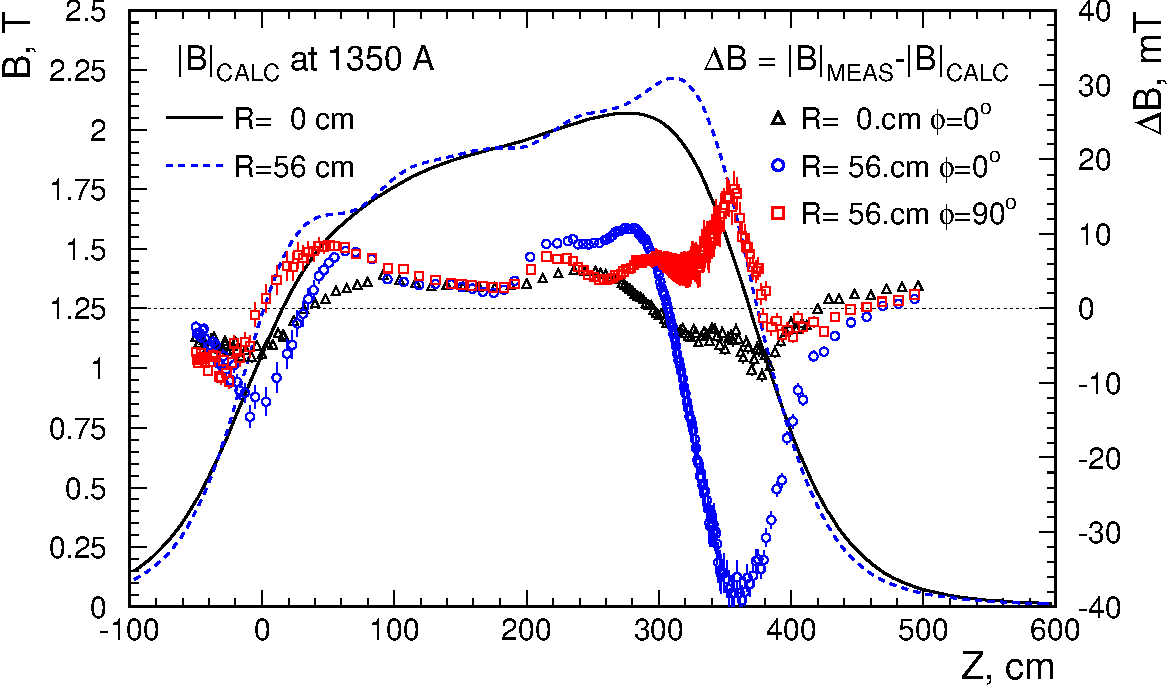
\includegraphics[angle=0,width=1.0\linewidth]{figures/solenoid_field_calc-meas_comparison_7_1_01}%
  \end{center}
  \caption{
    The full field at 1350~A calculated with {\it Poisson} (the left
    scale) at the axis and at the edge of the tracking fiducial volume
    - R=56~cm. The deviations of the measurements from the
    calculations are shown (the right scale) at the axis, as well as
    at R=56~cm. The measurements have been done at 6 azimuthal
    angles. Those demonstrating the largest deviations from the
    calculations - at 0$^\circ$ and 90$^\circ$ - are shown.  
%    In the area most important for tracking $45<Z<320$~cm the
%    deviations from the calculations are below 0.5\%.
    \label{fig:sol:field_comparison}
  }
\end{figure}


% ----------------------------------------------------------------------

\clearpage   % avoid formatting problems with empty sections
% %=======================+=========================
%================   Detector Overview ================
%=================================================

%\section[Detector overview (Curtis)]{Detector overview
\section[Detector overview]{Detector overview \label{sec:overview}}
The design of the GlueX detector \cite{Ghoul:2015ifw} is based on a solenoidal magnet that surrounds all detectors in the central region, providing a magnetic field of about $2$~T along the direction of the photon beam, which impinges on a 
$30$~cm-long\textcolor{blue}{(There was a question on the length of the target. Target section shows 30cm, but is it 29.25cm?)} liquid hydrogen target.  A schematic of the detector including its major sub-detectors is given in Fig.\,\ref{fig:layout_spectrometer}.

% ======================================================================================

\begin{figure*}[!htb]
\centering
  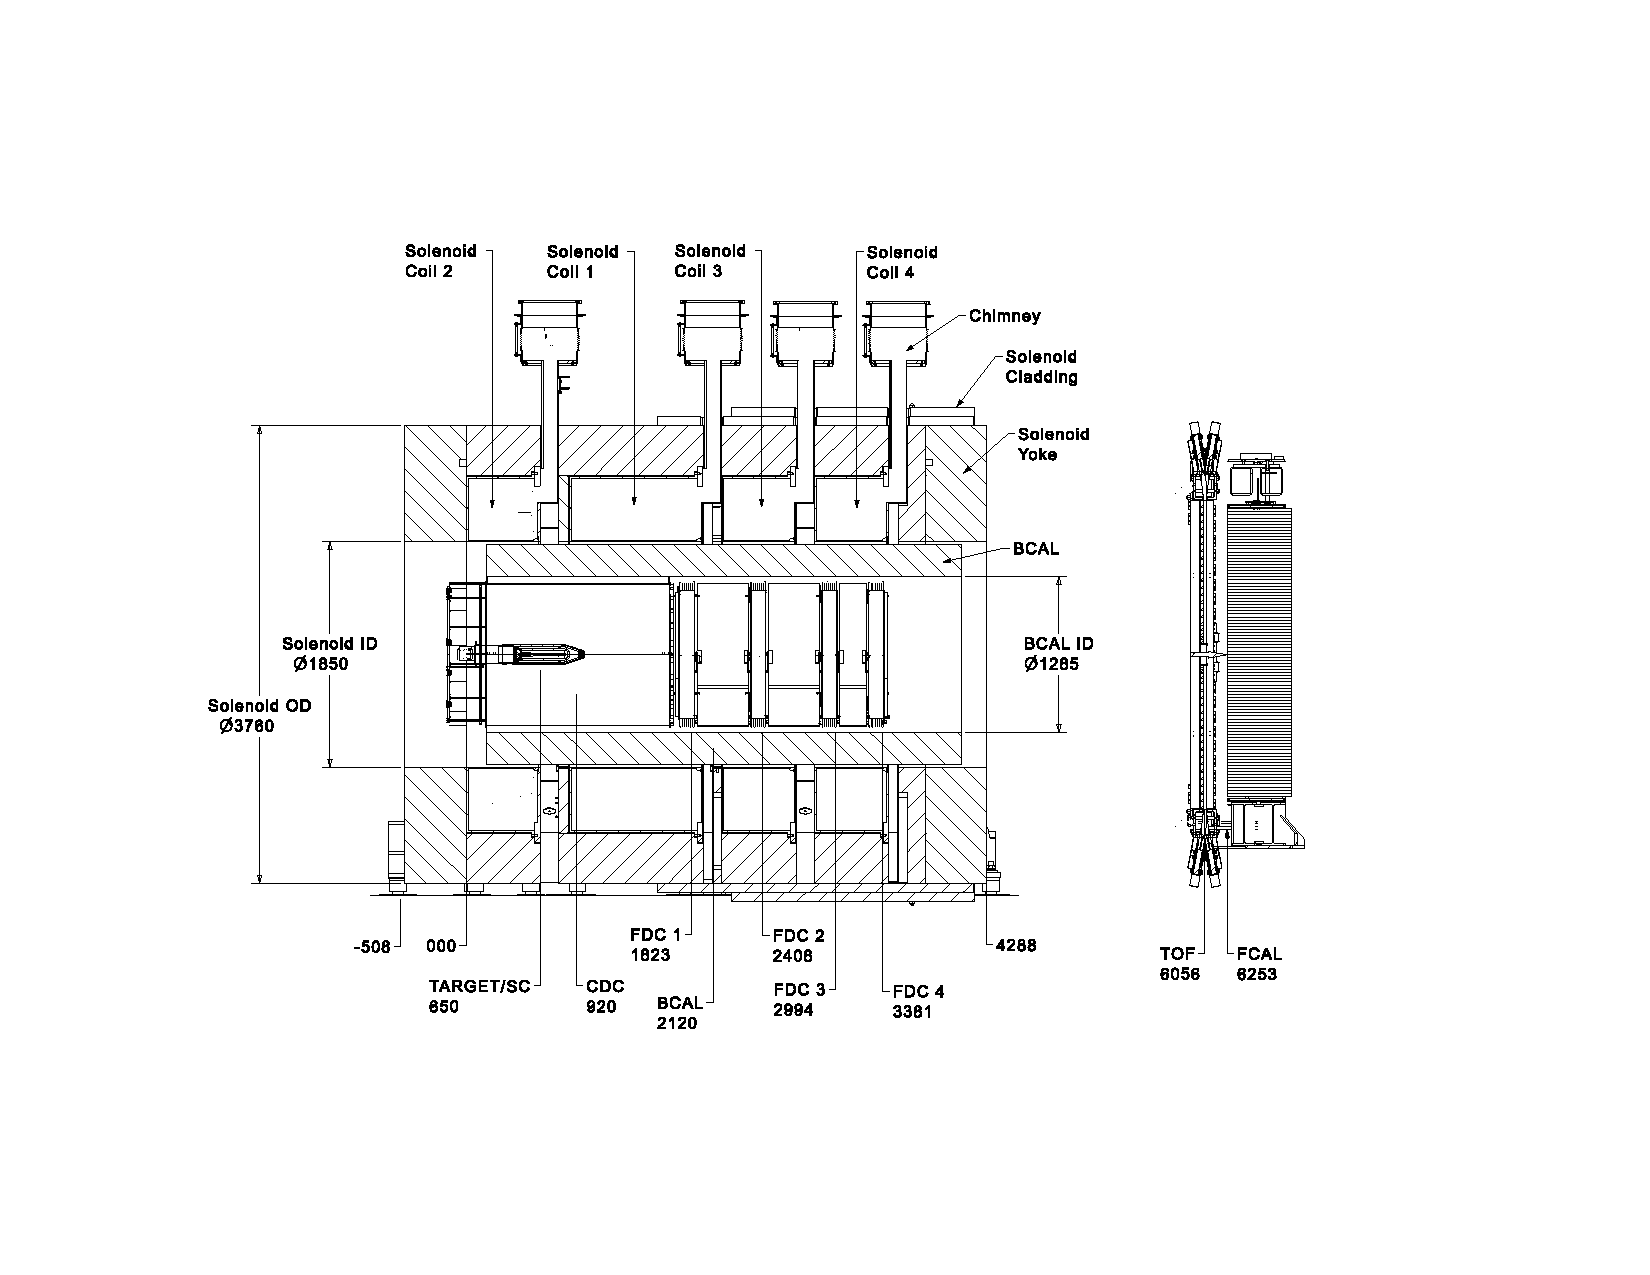
\includegraphics[angle=0,viewport=95 115 628 500,clip,width=1.0\linewidth]{figures/gluex_spectrometer_drawing_01_bw}%
  \caption[layout]{GlueX spectrometer layout. Dimensions are given in mm. The
    numbers show the Z-coordinates of the detectors' centers, or of
    the front face of the calorimeter modules in case of the FCAL.
    Glossary: 
              SC  - Start Counter (Section \ref{sec:st}), 
              CDC - Central Drift Chamber (Section \ref{sec:cdc}), 
              FDC - Forward Drift Chamber (Section \ref{sec:fdc}),
              BCAL - Barrel Calorimeter (Section \ref{sec:bcal}), 
              TOF -  Time-of-Flight hodoscope (Section \ref{sec:tof}), 
              FCAL - Forward Calorimeter (Section \ref{sec:fcal}).
%
%    \begin{tabular}{lll}
%       Name  & Detector & Section \\ \hline
%              SC  & Start Counter & \ref{sec:st} \\ 
%              CDC & Central Drift Chamber  & \ref{sec:cdc} \\ 
%              FDC & Forward Drift Chamber  & \ref{sec:fdc} \\ 
%              BCAL & Barrel Calorimeter    & \ref{sec:bcal} \\ 
%              TOF &  Time-of-Flight hodoscope & \ref{sec:tof} \\ 
%              FCAL & Forward Calorimeter    & \ref{sec:fcal} \\ 
%    \end{tabular}
    \label{fig:layout_spectrometer}
  }
\end{figure*}

% ======================================================================================

%\begin{figure}[tbp]
%\begin{center}
%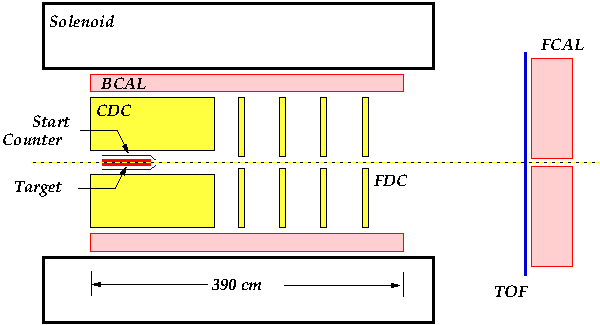
\includegraphics[width=0.7\textwidth]{figures/GlueX_Sketch.pdf}  
%\caption{\label{fig:gluexsketch}          
%  Sketch of GlueX detector.  The main systems of the detector are the Start %Counter \cite{Pooser:2019rhu}, the Central Drift Chamber (CDC) %\cite{VanHaarlem:2010yq} the Forward Drift Chamber (FDC) \cite{Pentchev2017281}, %a scintillator-based Time of Flight (TOF) wall and a lead-glass Forward %Calorimeter (FCAL) \cite{MORIYA201360}. The Barrel Calorimeter (BCAL) is %sandwiched between the drift chambers and the inner radius of the solenoid.  %(Color online)
%}   
%\end{center}  
%\end{figure}

\section[Target (C. Keith)]{Target \label{sec:target} }
A schematic diagram of the GlueX cryotarget is shown in Fig.~\ref{fig:Target}.  
The major components of the system are a pulse tube cryocooler,\footnote{Cryomech model PT415.}
a condenser, and a target cell.  These items are contained within
an aluminum and stainless steel `L'-shaped vacuum chamber
with an extension of closed-cell foam\footnote{Rohacell 110XT, Evonik Industries AG.}
surrounding the target cell.
In turn, the GlueX start counter (Sec.~\ref{sec:st}) surrounds the
foam chamber and is supported by the horizontal portion of the vacuum chamber.
Polyimide foils, 100$\mu$m thick, are used at the upstream and downstream ends of the
chamber as beam entrance and exit windows.
The entire system, including the control electronics, vacuum pumps,
gas-handling system, and tanks for hydrogen
storage, are mounted on a small cart that is attached to a set of rails for
insertion into the GlueX solenoid.  To satisfy the laboratory's flammable gas safety requirements,
the system is connected at multiple points to a nitrogen-purged ventilation pipe that
extends outside Hall D. 
\begin{figure*}
\begin{center}
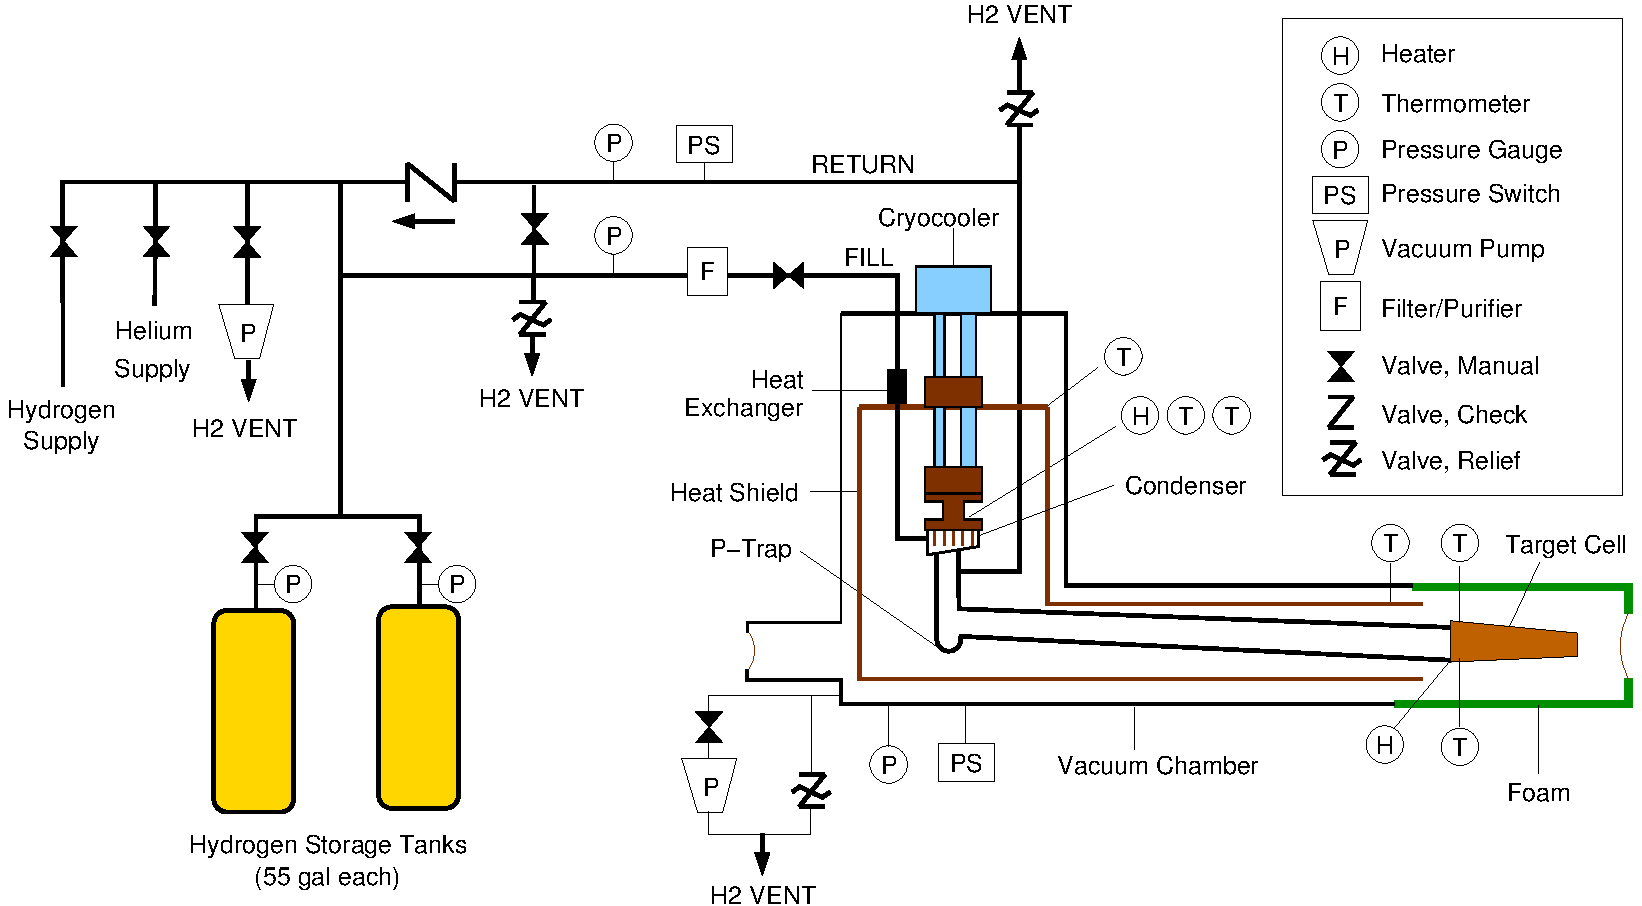
\includegraphics[width=5in]{figures/TargetSchematic2.pdf}
\end{center}
\caption{Simplified process and instrumentation diagram for the GlueX liquid hydrogen target (not to scale).
In the real system, the P-trap is above the level of the target cell and is used to
promote convective cooling of the target cell from room temperature.}
\label{fig:Target}
\end{figure*}

Hydrogen gas is stored inside two 200~l tanks and
is cooled and condensed into a small copper and stainless steel container,
the condenser, that is thermally anchored to the second cooling stage of the cryocooler. 
The first stage of the cryocooler is used to
cool the H$_2$ gas to about 50~K before it enters the condenser.
It also cools a copper thermal shield that surrounds all
lower temperature components of the system except for the
target cell itself, which is wrapped in a few layers of aluminized-mylar/cerex insulation.

The condenser is comprised of a copper C101 base
sealed to a stainless steel can with an indium o-ring.  Numerous vertical 
fins are cut into the copper base, giving a large surface area for condensing hydrogen gas.
A heater and a pair of calibrated cernox thermometers\footnote{Lake Shore Cryotronics.}
are attached outside the condenser and are used to regulate its temperature when the
system is filled with liquid hydrogen.

The target cell, shown in Fig.~\ref{fig:TargetCell}, is similar to
designs utilized in Hall B at Jefferson Lab for many years~\cite{HAKOBYAN2008218}.  
The cell walls are made from 100~$\mu$m thick aluminized
polyimide sheet that is wrapped in a conical shape and glued along the edge,
overlapping in a 2~mm wide scarf joint.  
The conical shape prevents bubbles from collecting inside the cell, while the
scarf joint reduces the stress riser at the glue joint.  This conical
tube is glued to an aluminum base 
along with stainless steel fill and return tubes leading to the condenser, a feed-thru for two
calibrated cernox thermometers inside the cell, and a
polyamide-imide support for the reentrant, upstream beam window.  
Both the upstream and downstream beam
windows are made of non-aluminized,
100~$\mu$m thick polyimide films that have been extruded into the
shapes indicated in Fig.~\ref{fig:TargetCell}. All items are glued together using
a two-part epoxy\footnote{3M Scotch-Weld epoxy adhesive DP190 Gray.}
that has been in reliable use at cryogenic temperatures at
Jefferson Lab for many years. 
A second  heater is attached to the aluminum base and
is used to boil the liquid from the cell for empty target measurements.
The base is attached to a kinematic mount which is in turn
supported inside the vacuum chamber using a system of carbon fiber rods.    
The mount is used to correct the pitch and yaw
of the cell, while $x$, $y$, and $z$ adjustment 
is accomplished using positioning screws on the target cart. 


During normal operation sufficient hydrogen gas is condensed from the storage tanks
until the target cell, condenser, and interconnecting piping are filled with liquid hydrogen
and an equilibrium pressure of about 20~psia is achieved.  
The condenser temperature is regulated at 18~K, while the
liquid in the cell cools to about 19.8~K.  This is 1.5~K below the saturation
temperature of H$_2$ and eliminates boiling within the cell, thus permitting a more
accurate determination of the fluid density.  
The system can be cooled from room temperature and filled with liquid hydrogen in
about six hours.
For empty target runs, the liquid in the system is boiled back into the storage tanks using the heater
attached to the cell's aluminum base, which takes about five minutes.  During this
mode of operation, H$_2$ gas continues to condense and drain towards the target cell, where it
is evaporated by the cell heater.  In this way, the cell does not warm above 40~K, and
it can be re-filled with liquid hydrogen in about twenty minutes.

\begin{figure}
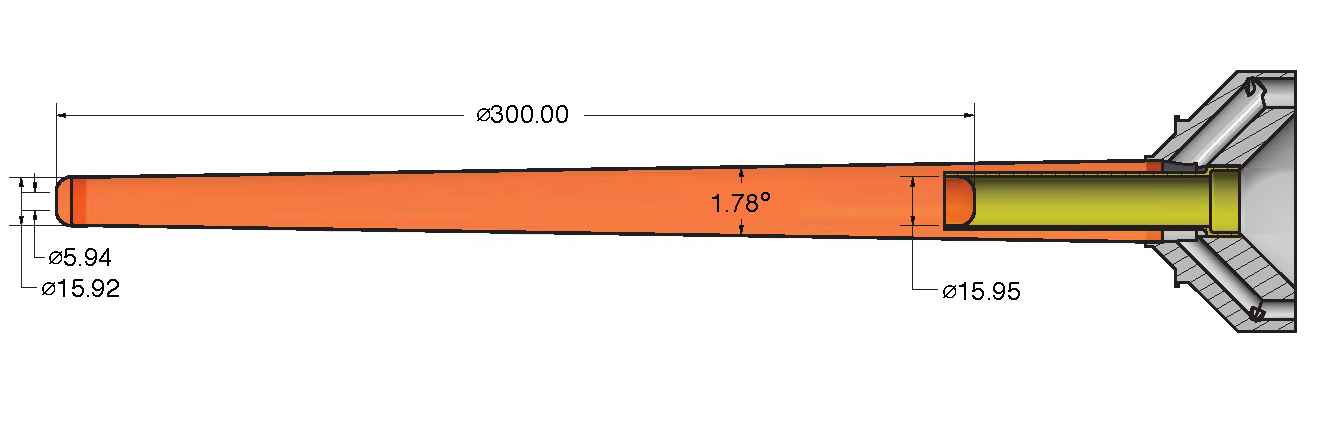
\includegraphics[width=3.5in]{figures/GluexCell_mm.pdf}
\caption{Target cell for the liquid hydrogen target.  Dimensions are in mm.  The photon beam
tranverses the target right to left in this drawing.}
\label{fig:TargetCell}
\end{figure}

The cryotarget is controlled using a
National Instruments CompactRIO 9030, which is an industrial embedded controller 
capable of running LabVIEW programs on top of an AMD64 Linux environment. 
Control logic and equipment interface is handled by a LabVIEW program, 
while a standard EPICS softIOC running in Linux provides a
bridge between the controller and JLab's EPICS enviroment. The LabVIEW program interacts
with the softIOC using National Instrument's DSC module.    
Temperature read back and control of the condenser and target cell thermometers
are managed by a four-input temperature
controller with PID control loops of 50 and 100~W\footnote{Lake Shore Model 336.}.
Strain gauge pressure sensors measure the fill and return pressures with 0.25\% 
accuracy.  

Operation of the cryotarget is highly automated and requires minimal user intervention.
Most tasks can be performed by pressing one of two main buttons on
the Graphical User Interface: {\bf Fill Target} and {\bf Empty Target}.
Each button checks the status of the cryocooler, hydrogen gas pressure, insulating vacuum, etc.\
and loads appropriate settings for alarm values and temperature-control set points.  
When the expected equilibrium readings for a full (or empty) target are achieved, the
GUI informs the user that the target is stable and ready for beam.  A third button, {\bf Target Off},
simply turns off the cryocooler and allows the system to warm over the course of a few days.

The GlueX cryotarget has operated in a very reliable and predictable manner throughout the
experiment.  When filled with subcooled liquid, its long-term temperature ($\pm 0.2$~K) and
and pressure ($\pm 0.1$~psi) stability enable a determination of the liquid density to better than 0.5\%.
It has also demonstrated the capability to condense helium
in the target cell and operate in a stable manner at 4.2~K.  However, this requires extending the
thermal shield to surround the target cell. A thin (1~mm) aluminum shell, clamped to the end
of the existing copper shield is sufficient for this purpose.

\section{Tracking detectors \label{sec:tracking}}
\subsection[Central drift chamber (Naomi)]{Central drift chamber \label{sec:cdc}}

The Central Drift Chamber (CDC) is a cylindrical straw-tube drift chamber which is used to track charged particles, providing timing and energy loss measurements~\cite{GlueXCDCNIM}.
It is situated inside the Barrel Calorimeter, surrounding the target and start counter, and upstream of the Forward Drift Chambers. 
All of these are inside the solenoid. 
The active volume of the CDC is traversed
by particles coming from the target with polar angles between $6^{\circ}$ and $168^{\circ}$, with optimum 
coverage for polar angles between $29^{\circ}$ and $132^{\circ}$.  

The CDC contains 3522 Mylar\footnote{www.mylar.com} straw tubes of diameter 1.6~cm in $28$ layers,
located in a cylindrical volume which is 1.5~m long, with an inner radius of 10~cm and outer radius of 56~cm, as measured from the beam-line.  
The straws are arranged in 28 layers; 22 of these are axial and 16 are at stereo angles of $\pm 6^{\circ}$ to provide position information in the beam direction. Fig.\,\ref{fig:CDC_stereotubes}  shows the CDC during construction. 

\begin{figure}[tbp]
\begin{center}
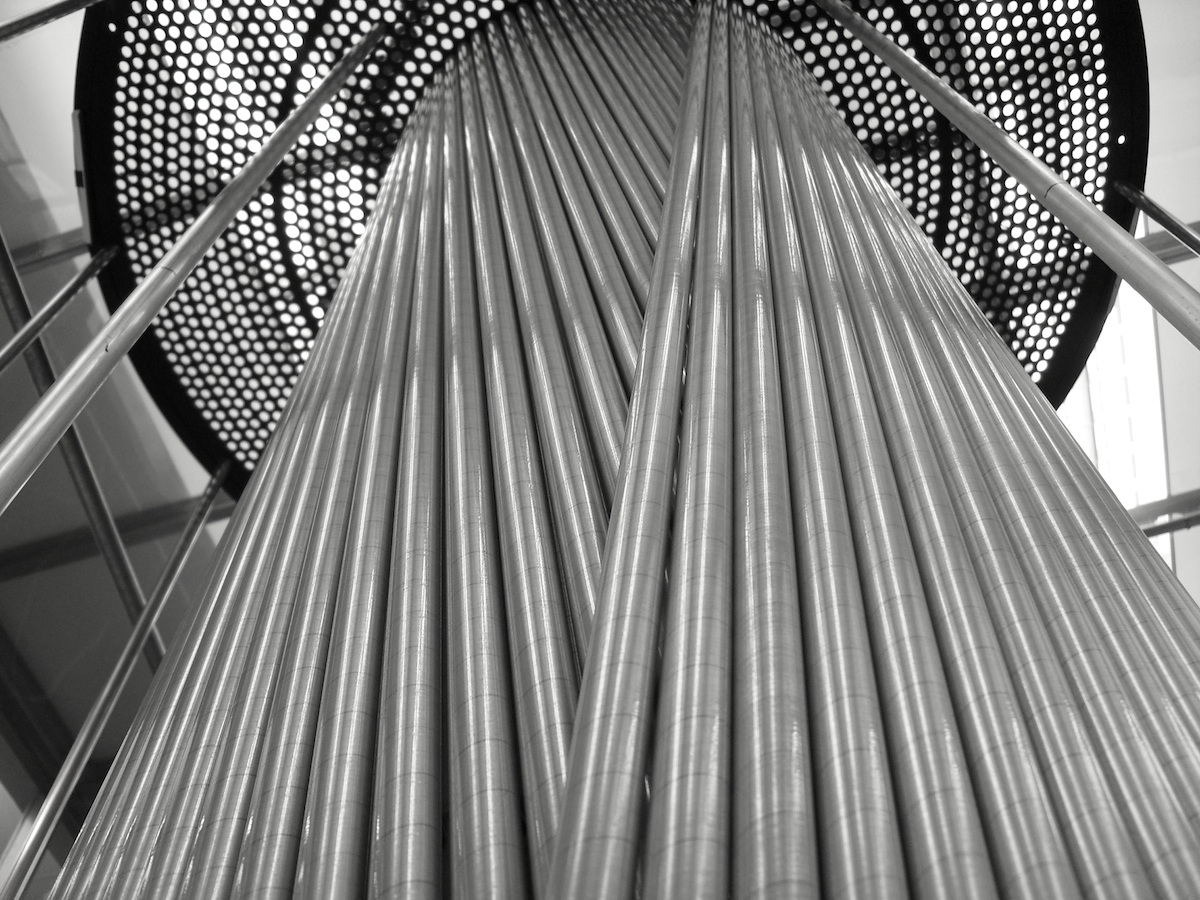
\includegraphics[width=0.7\textwidth]{figures/CDC_stereotubes}  
\caption{\label{fig:CDC_stereotubes}          
  The Central Drift Chamber during construction. A partially completed layer of stereo tubes is shown, surrounding a layer of tubes at the opposing stereo angle. Part of the carbon fiber endplate, some temporary support rods and some of the 12 rods linking the two endplates are also shown.}  
\end{center}
\end{figure}

The volume surrounding the straws is enclosed by an inner cylindrical wall of G10, an outer cylindrical wall of aluminum, and two circular endplates. 
The upstream endplate is made of aluminum, while the downstream endplate is made of carbon fiber. The endplates are connected by 12 aluminum support rods. 
Holes milled through the endplates support the ends of the straw tubes, which are glued into place using several small components per tube.  
These components also support the anode wires, which are 20~$\mu$m diameter gold-plated tungsten, installed with 30~g tension.
At the upstream end these components are made of aluminum and were glued in place using conductive epoxy\footnote{3M Scotch-Weld DP-460NS, www.3m.com}. 
This provides a good electrical connection to the inside walls of the straw tubes, which are coated in aluminum.
The components at the downstream end are made of Noryl plastic\footnote{www.sabic.com} and were glued in place using conventional non-conductive epoxy\footnote{3M Scotch-Weld 920-H, www.3m.com}.
The materials used for the downstream end were chosen to be as lightweight as feasible so as to minimize the energy loss of charged particles passing through them. 

At each end of the chamber there is a cylindrical gas plenum outside the end-plate; the downstream plenum is 2.54~cm deep, with a sidewall of ROHACELL\footnote{www.rohacell.com} and a final outer wall of aluminized Mylar film, and the upstream plenum is 3.18~cm deep, with a polycarbonate sidewall and a polycarbonate disc as its outer wall. 
Five thermocouples are located in each plenum and used to monitor the temperature of the gas.
The gas mixture used is 50$\%$ argon and 50$\%$ carbon dioxide, at atmospheric pressure, with a small admixture of isopropanol to delay aging.
The gas supply runs in 12 tubes through the volume surrounding the straws into the downstream plenum. 
There it enters the straws and flows through them into the upstream plenum. From the upstream plenum the gas flows into the volume surrounding the straws, and from there it exhausts to the outside, bubbling through small jars of mineral oil.

The readout wires pass through the polycarbonate disc and the upstream plenum to reach the anode wires. 
They are connected in groups of 20 to 24 to transition boards which are mounted onto the polycarbonate disc. 
Preamplifiers\cite{hdnote2515} are mounted on high voltage boards which are bolted onto the transition boards. The aluminum endplate, outer cylindrical wall of the chamber, aluminum components connecting the straws to the aluminum endplate and the inside walls of the straws are all connected to a common electrical ground. 
The anode wires are held at +2.1kV during normal operation. 

Fig.\,\ref{fig:CDC_rhs}  shows the CDC during initial readout tests 
\begin{figure}[tbp]
\begin{center}
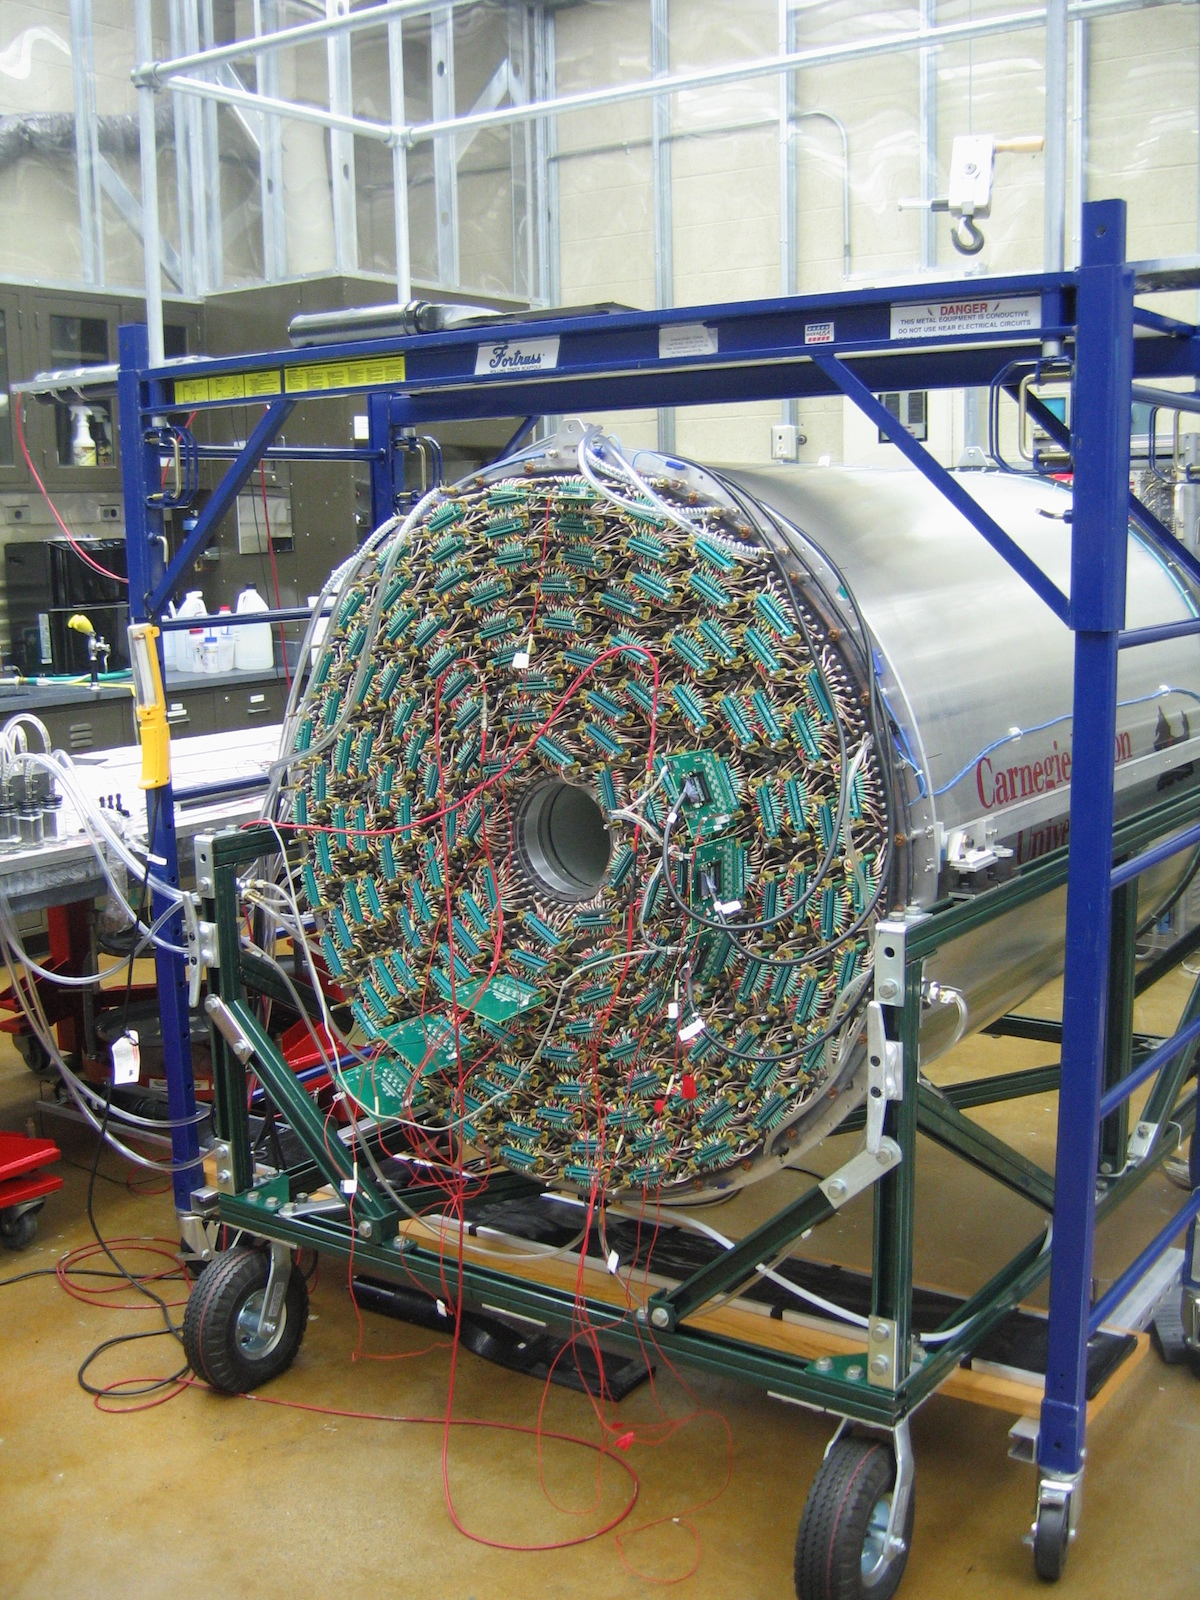
\includegraphics[width=0.7\textwidth]{figures/cdc_rhs.jpg}  
\caption{\label{fig:CDC_rhs}          
  The Central Drift Chamber during initial readout tests. Several HVBs and preamplifiers and many transition boards are visible.}
  \end{center}
\end{figure}


\subsection[Forward drift chambers (Lubomir)]{Forward drift chambers
\label{sec:fdc} }

The Forward Drift Chamber (FDC) system consists of 24 disk-shaped planar drift chambers of 1m-diameter.
They are grouped into four packages inside the bore of the spectrometer magnet.
Due to the high particle density in the forward region the tracking there requires
good multi-track separation.
This is achieved with additional cathode strips on both sides of the wire plane allowing for a  reconstruction of a space point on the track from each chamber. 
The FDC registers tracks with polar angles as low as $1^\circ$ and up to $10^\circ $
with all the chambers, while having partial coverage up to $20^\circ$.

One FDC chamber consists of a wire plane and two cathode planes on both sides at a distance of $5$~mm from the wires (Fig.~\ref{FDC_OneCell}).
\begin{figure}[tbp]
\begin{center}
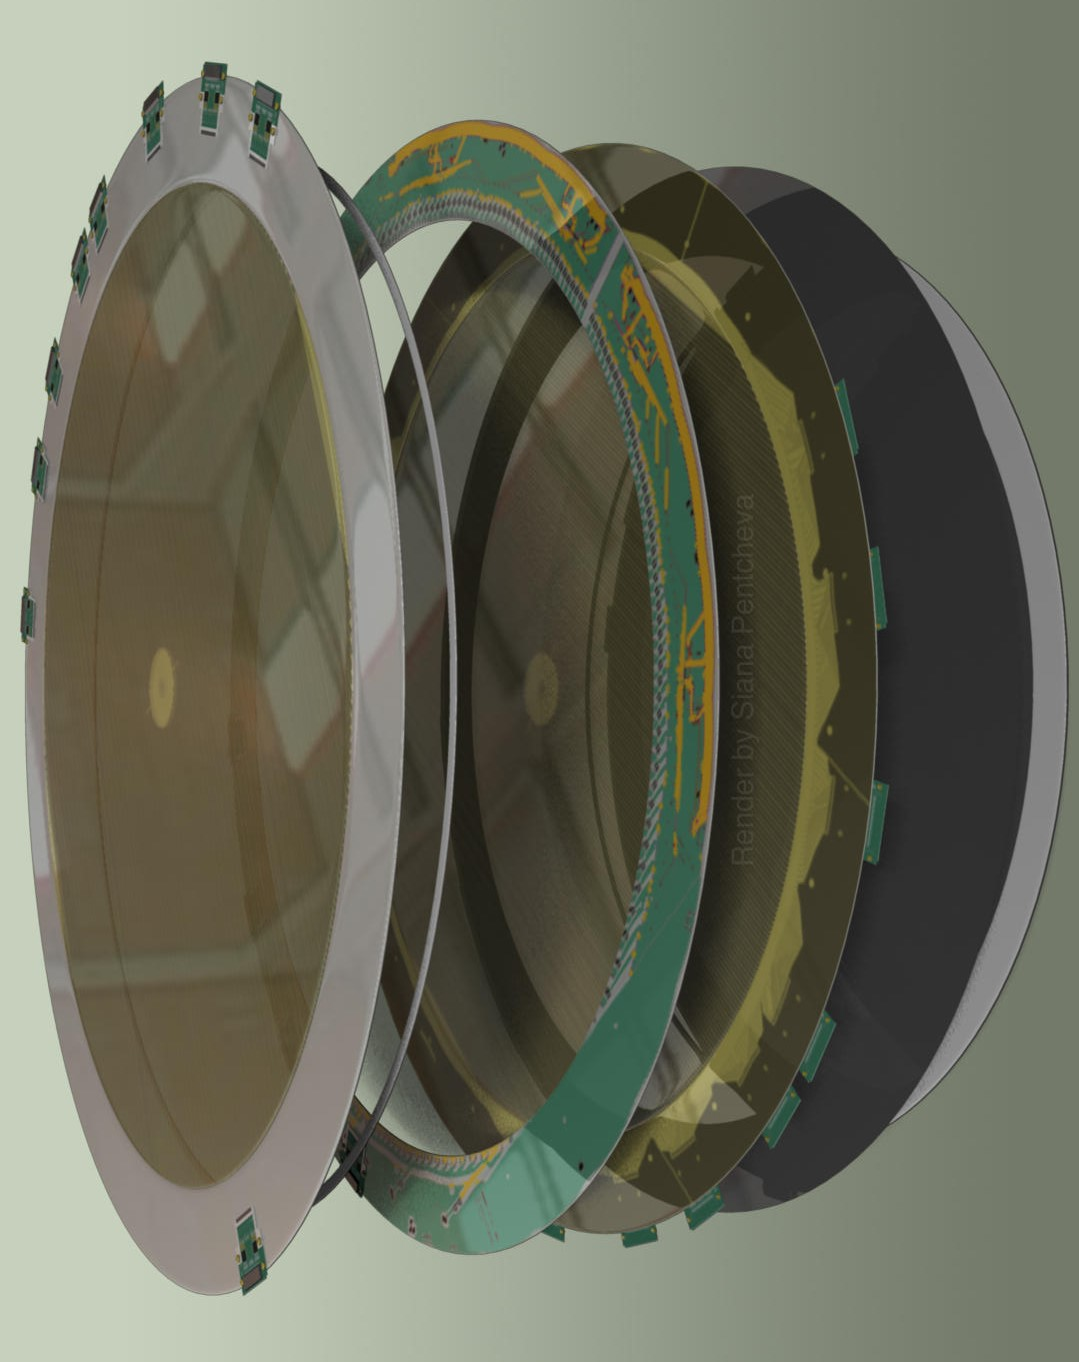
\includegraphics[width=0.75\textwidth]{figures/FDC_OneCell.jpg}  
\caption{\label{FDC_OneCell}
Artistic view of one FDC chamber (from left to right): upstream cathode, wire plane, downstream cathode, chamber separator.
}
\end{center}
\end{figure}
To minimize the material and allow registration of low energy photons by the outside e.m. calorimeters,
the frame that holds the wires is made out of Rohacell with a thin G10 skin.
The wire plane has sense ($20~\mu$m diameter) and field ($80$~$\mu$m) wires $5$~mm apart, forming a field cell of $10\times 10$~mm$^2$. 
The gas mixture used is $40\%$~Ar and $60\%$~CO$_2$.
A positive HV of about $2.2$~kV is applied on the sense wires and negative of $0.5$~kV on the field ones. 
The cathodes are made out of $2$-$\mu$m-thin $Cu$ strips on Kapton foil with a pitch of $5$~mm and are held on ground. The strips on the two cathodes are at $30^\circ $ bewteen each other and at $75^\circ $ and $105^\circ $ angle w.r.t. the wires.

The six chambers of a package are separated by thin aluminized Mylar.
Each chamber is rotated w.r.t. the previous one by $60^\circ $.
The total material of a package in the sensitive area is $0.43\%$~R.L. and about half of that in the area along the beam line that has no copper on the cathodes.
The sense wires in the inner area of $6-7.8$~cm diameter (depending on the distance of the package to the target) are thickened from $20$~$\mu$m to $\sim 80$~$\mu$m which makes them insensitive to the high raters along the beam.
The distance between the first and last package is $169$~cm. 
All the chambers are supplied with gas in parallel. 
In total $2,304$ wires and $10,368$ strips are read using charge pre-amplifiers with $10$~ns peaking time with a gain of $0.77$~mV/fC for the wires and $2.6$~mV/fC for the strips.

\subsection{Electronics \label{sec:dcelectronics}}
The high voltage (HV) supply units used are CAEN A1550P with noise-reducing modules added to each crate chassis. 
The low voltage (LV) supplies are MPOD MPV8008. 
The preamplifiers are a custom JLab design based on an ASIC~\cite{hdnote2515}
with 24 channels per board; they are charge-sensitive, and are capacitatively coupled to the wires in the CDC and FDC and directly coupled to strips in the FDC. 

Pulse information from the CDC anode wires and FDC cathode strips is obtained and read out using 72-channel 125 MHz 12-bit flash ADCs \cite{Visser2008,5873864}. 
Each fADC receives signals from three preamplifiers. 
The signal cables from different regions of the drift chambers are distributed between the fADCs in order to share out the processing load as evenly as possible.  

The fADC firmware is activated by a signal from the GlueX trigger. It then computes the following for the next pulses observed above a given threshold within a given time window: pulse number, arrival time, pulse height, pulse integral, pedestal height immediately before the pulse, and a quality factor indicating if the arrival time is likely to be less accurate than usual. 
Signal filtering and interpolation is used to obtain the arrival time to the nearest 0.8~ns. 
The firmware performs these calculations for the CDC and FDC alike, and uses different readout modes to provide the data with the precision required by the separate detectors. 
For example, the CDC electronics read out only one pulse but requires both pulse height and integral, while the FDC electronics read out up to 4 pulses and do not require pulse integral.  


The FDC anode wires are read out using the GlueX f1TDC\cite{JLAB2002}. 



\subsection[Gas system (Beni)]{Gas system \label{sec:gas}}
Both tracking chambers the CDC and FDC operate with the same type of gases, argon and CO$_{2}$. Since the relative mixture of
the two gases are slightly different for the two tracking chambers the gas system has two separate identical mixing stations. There is one gas supply of argon and CO$_{2}$ for both mixing stations. A limiting opening in the supply
lines provide over-pressure protection to the gas system and filters in the gas lines provide protection against potential
pollution of the gas from the supply. Both gases are mixed together using mass flow controllers (MFC) that can be 
configured
to provide the desired mixing ratio of argon and CO$_{2}$.  The MFC as well as the related control electronics is from
BROOKS Instruments~\cite{BrooksInst}.
The mixed gas is filled into storage tanks one for the CDC one for the FDC. Their pressure is
regulated by controlling the operation of the MFCs with a logic circuit based on Allen-Bradley control logics~\cite{AllenBradley} 
that are used throughout the experimental hall and keeps
the pressure in the tank between 10 and 12~psi. The tank serves as a reservoir and buffer.
A safety relieve valve on each tank
provides additional protection against over pressure. While the input pressure to the MFC is at 40~psi the pressure after
the MFC is designed to be always below 14~psi above atmospheric pressure. After the mixing tank there is a provision
built into the system to let the gas pass through an alcohol bath to add a small amount to the gas mixture.
This small admixture of alcohol will protect the wire chambers from aging effects caused by radiation exposure from the beam.
This part of the gas system is located above ground in a separate gas shed before the gas mixture is transported
to the experimental hall via polyethylene pipes.

Down in the hall additional MFC allow to specify the exact amount of gas to be provided to the chambers. One for the CDC
and four for the individual FDC packages. The CDC is operated with a flow of 1~l/m while each FDC package is operated with
a flow of 0.1~l/m. To protect the chambers from over-pressure there is a bypass line at the input to the detectors that
is open to atmosphere after a bath of mineral oil. The height of the oil level determines the maximum possible gas pressure at
the input to the chambers. There is a second mineral oil bath at the output to protect against possible air back-flow into
the chamber. Its height of oil above the exhaust line determines the operating pressure inside the chambers.

Pressure tabs are mounted at many places in the gas system to monitor the pressure during operation. Among these are
6 pressure tabs for each FDC chamber to monitor the pressure in each individual plane. The CDC gas pressure is monitored
at the input, the down stream gas plenum and at the exhaust.

There is an additional tab in the exhaust line that can be used to divert some gas from the chamber exhaust to be connected
to an oxygen sensor to test the amount of oxygen in the gas. Too much oxygen in the gas will degrade the gain of
the chambers and reduce the tracking efficiency. The oxygen levels found in the chamber are below 100~ppm. 

\subsection{Calibration, performance and monitoring \label{sec:dccalib}}
Time calibrations for the drift chambers are used to remove the time offset due to the electronics, so that after calibration the earliest possible arrival time of the pulse signals is at 0~ns. These offsets and the function parameters used to describe the relationship between the pulse arrival time and the closest distance between the track and the anode wire are obtained for each session of data-taking. 

The CDC gain calibration procedure entails matching the position of the minimum ionizing peak for each of the 3522 straws, and then matching the dE/dx at 1.5~GeV/c to the calculated value of 2.0~ keV/cm. This takes place during the early stages of data analysis. Gain calibration for the individual wires is performed each time the HV is switched on and whenever any electronics modules are replaced. Gain calibration for the chamber as a whole is performed for each session of data-taking; these are limited to two hours as the gain is very sensitive to the atmospheric pressure. Position calibrations were necessary to describe the small deflection of the straw tubes midway along their length; these were performed in 2016 and repeated in 2017, with no significant difference found between the two sets of results.  Position resolution from the CDC is of the order of 130~$\mu$m and its detection efficiency per straw is over 98\% for tracks up to 4~mm from the wire. The efficiency decreases as the distance between the track and the wire increases, but the close-packing arrangement of the straw tubes and the large number of straws traversed by each track compensate for this. 

For the FDC system, an internal per chamber calibration process is first performed to optimize the track position information obtained.  
In the FDC the avalanche created around the wire is seen in three projections: on the two cathodes and on the wires.
The drift time information from the wires is used to reconstruct the hit position perpendicular to the wire.
The strip charges from the two cathodes are used to reconstruct the avalanche position along the wire. 
The same strip information can be used to reconstruct the avalanche position perpendicular to the wire which, due to the proximity of the avalanche to the wire, is practically the wire position as illustrated in Fig~\ref{FDC_wires_from_strips}.
\begin{figure}[tbp]
\begin{center}
%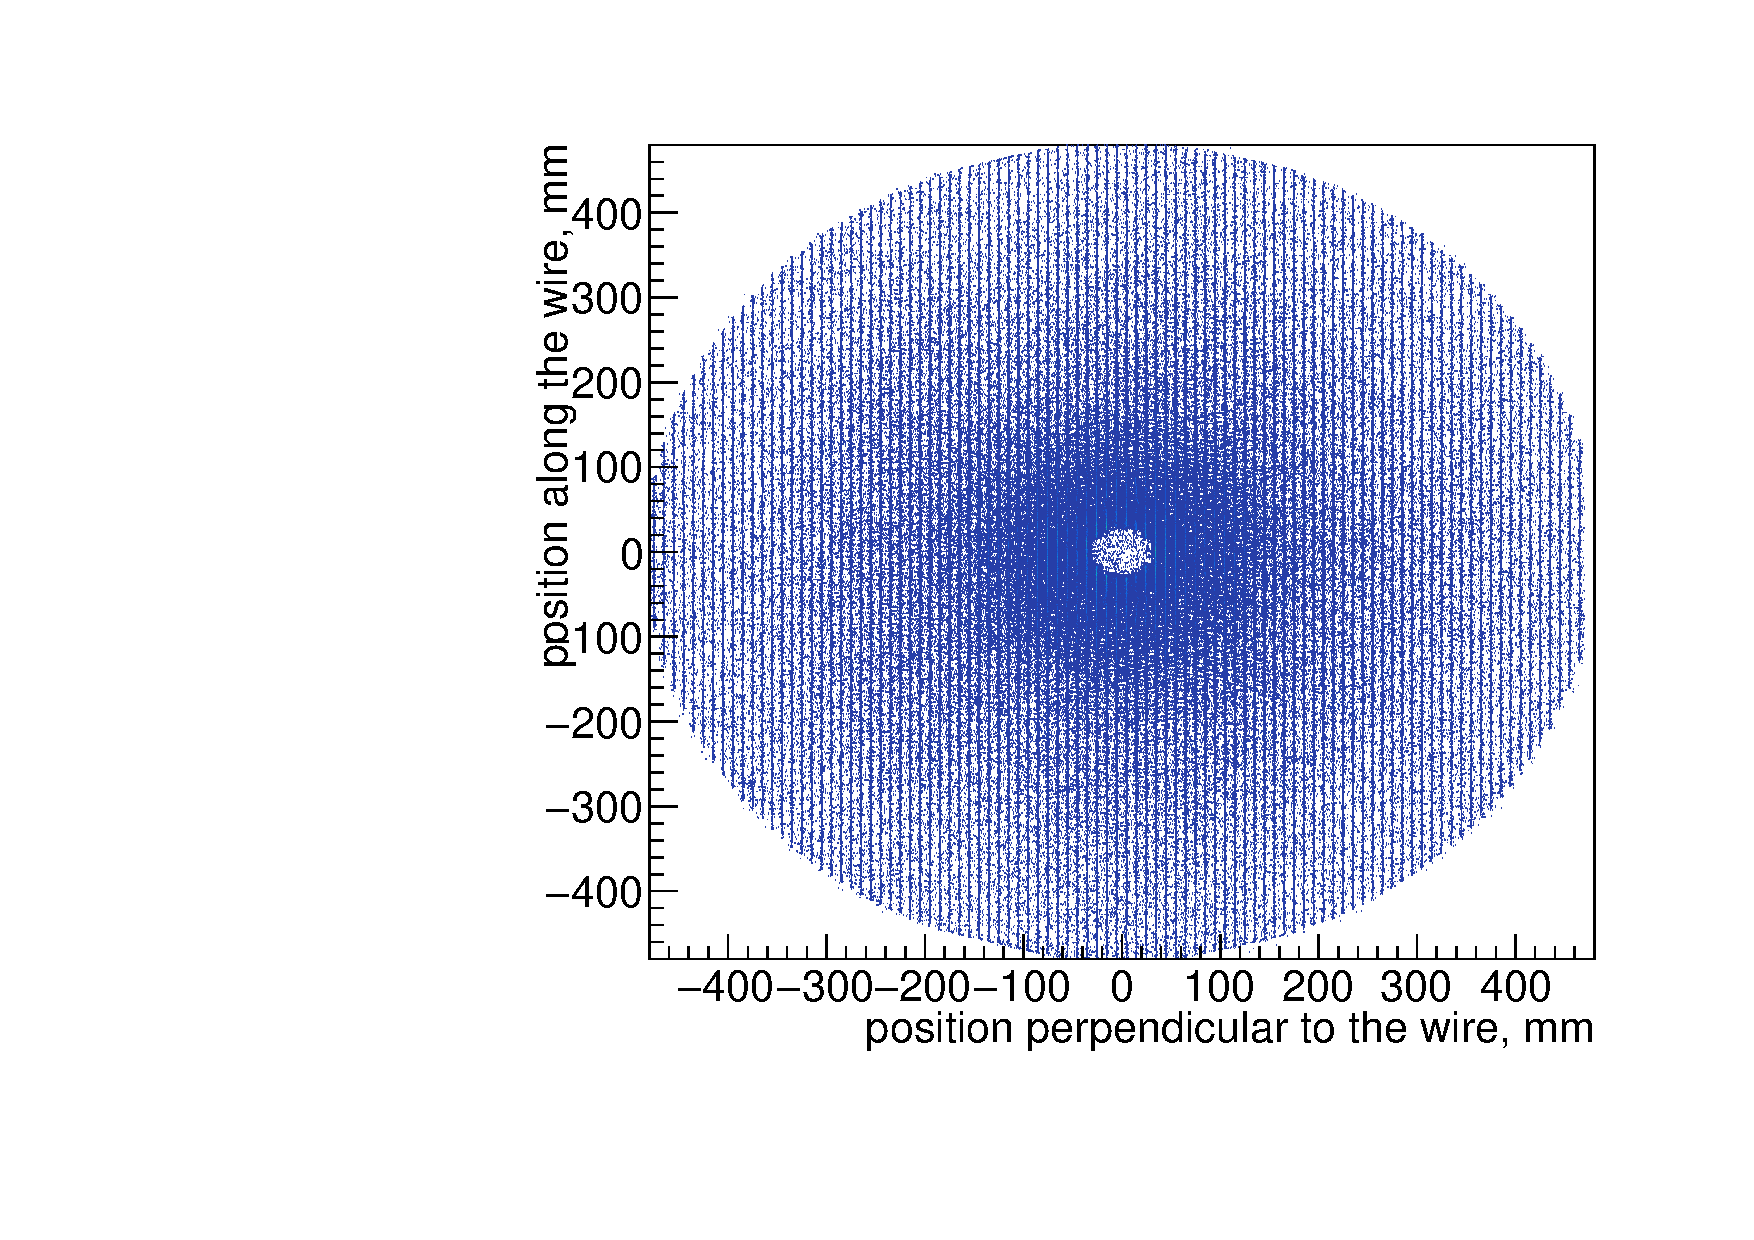
\includegraphics[width=0.95\textwidth]{figures/FDC_wires_from_strips.pdf}  
\caption{\label{FDC_wires_from_strips} Wire (avalanche) positions reconstructed from the strip information on the two cathodes in one FDC chamber.
}   
\end{center}  
\end{figure}
This is used to align the strips on the two cathodes w.r.t. the wires. 
At the same time the residuals of the reconstructed wire positions are an estimate of the strip resolution.
The resolutions of the detector were reported earlier \cite{FDC_NIM}. 
The strip resolution along the wires estimated from the wire position reconstruction, varies between $180$ and $80$~$\mu$m depending on the total charge induced on the strips. The drift distance is reconstructed from the drift time with a resolution between $240$ and $140$~$\mu$m
depending on the distance of the hit to the wire in the $0.5-4.5$~mm range.  

Position offsets and package rotations were determined for both drift chamber systems, first independently, and then together, using the alignment software MILLEPEDE\cite{millepede} in a process described in \cite{GlueXCDCNIM} and in \cite{MikeStaib_thesis}.

Online monitoring software enables the shift-takers to check that the number of channels recording data, the distribution of signal arrival times and the dE/dx are as expected. 




\subsection{Summary \label{sec:dcsummary}}
 

\section[Performance of the charged particle tracking system (Simon)]{Performance of the charged particle tracking system \label{sec:trackingperformance}}
\subsection{Track reconstruction}

The first stage in track reconstruction is pattern recognition.  Hits in adjacent
 layers in the FDC in each package are formed into track segments that are 
linked together with other segments in other packages to form FDC track 
candidates using a helical model for the track parameters.
Hits in adjacent rings in the axial layers of the CDC are also associated into 
segments that are linked together with other segments in other axial layers
and fitted with circles in the projection perpendicular to the beam line. We 
then find intersections between these circles and the stereo wires and perform 
a linear fit to find a z-position near the beam line and the tangent to the dip
 angle $\lambda=\pi/2-\theta$.  These parameters in addition to the circle fit 
parameters form a CDC track candidate for each set of linked axial and stereo 
layers.   We link FDC and CDC track candidates together that emerge from the 
target in the $\theta=5^\circ-20^\circ$ range that pass through both the FDC 
and the CDC.

The second stage uses a Kalman Filter \cite{KalmanFilter, KalmanFilter2} to find the fitted track parameters
\{z,D,$\phi$,$\tan\lambda$,$q/p_T$\}
at the position of closest approach of the track to the beam line using the 
track candidate parameters as an initial guess.  Here $D$ is the signed 
distance of closest approach to the beam line.  The Kalman Filter proceeds in 
steps from
the hits farthest from the beam line toward the beam line, taking into account
energy loss and multiple scattering at each step along the way and incorporating
a map of the magnetic field within the bore of the solenoid magnet.  For the 
first 
initial pass of the filter we do not use the drift time information from the 
wires.  We assume that each particle is a pion, except for low momentum track 
candidates (p$<$0.8 GeV/c), for which we redo the fits with a proton hypothesis.

At the beginning of the third stage we match each fitted track from the second 
stage to the start counter, the time-of-flight scintillators, the BCAL and the 
FCAL to determine a start time $t_0$ so that the drift time to each wire 
associated with the track can be used in the fit.  Each track is refitted with
the drift information multiple times using the set \{$e^\pm,\pi^\pm,K^\pm,p^\pm$\} 
of mass hypotheses.




\subsection{Momentum resolution}

The momentum resolution as a function of angle and magnitude for pions and 
protons is shown in Fig.~\ref{fig:dp_p}.  The angular resolution is shown in 
Fig.~\ref{fig:angle res}.


\begin{figure}[tbp]
\begin{center}
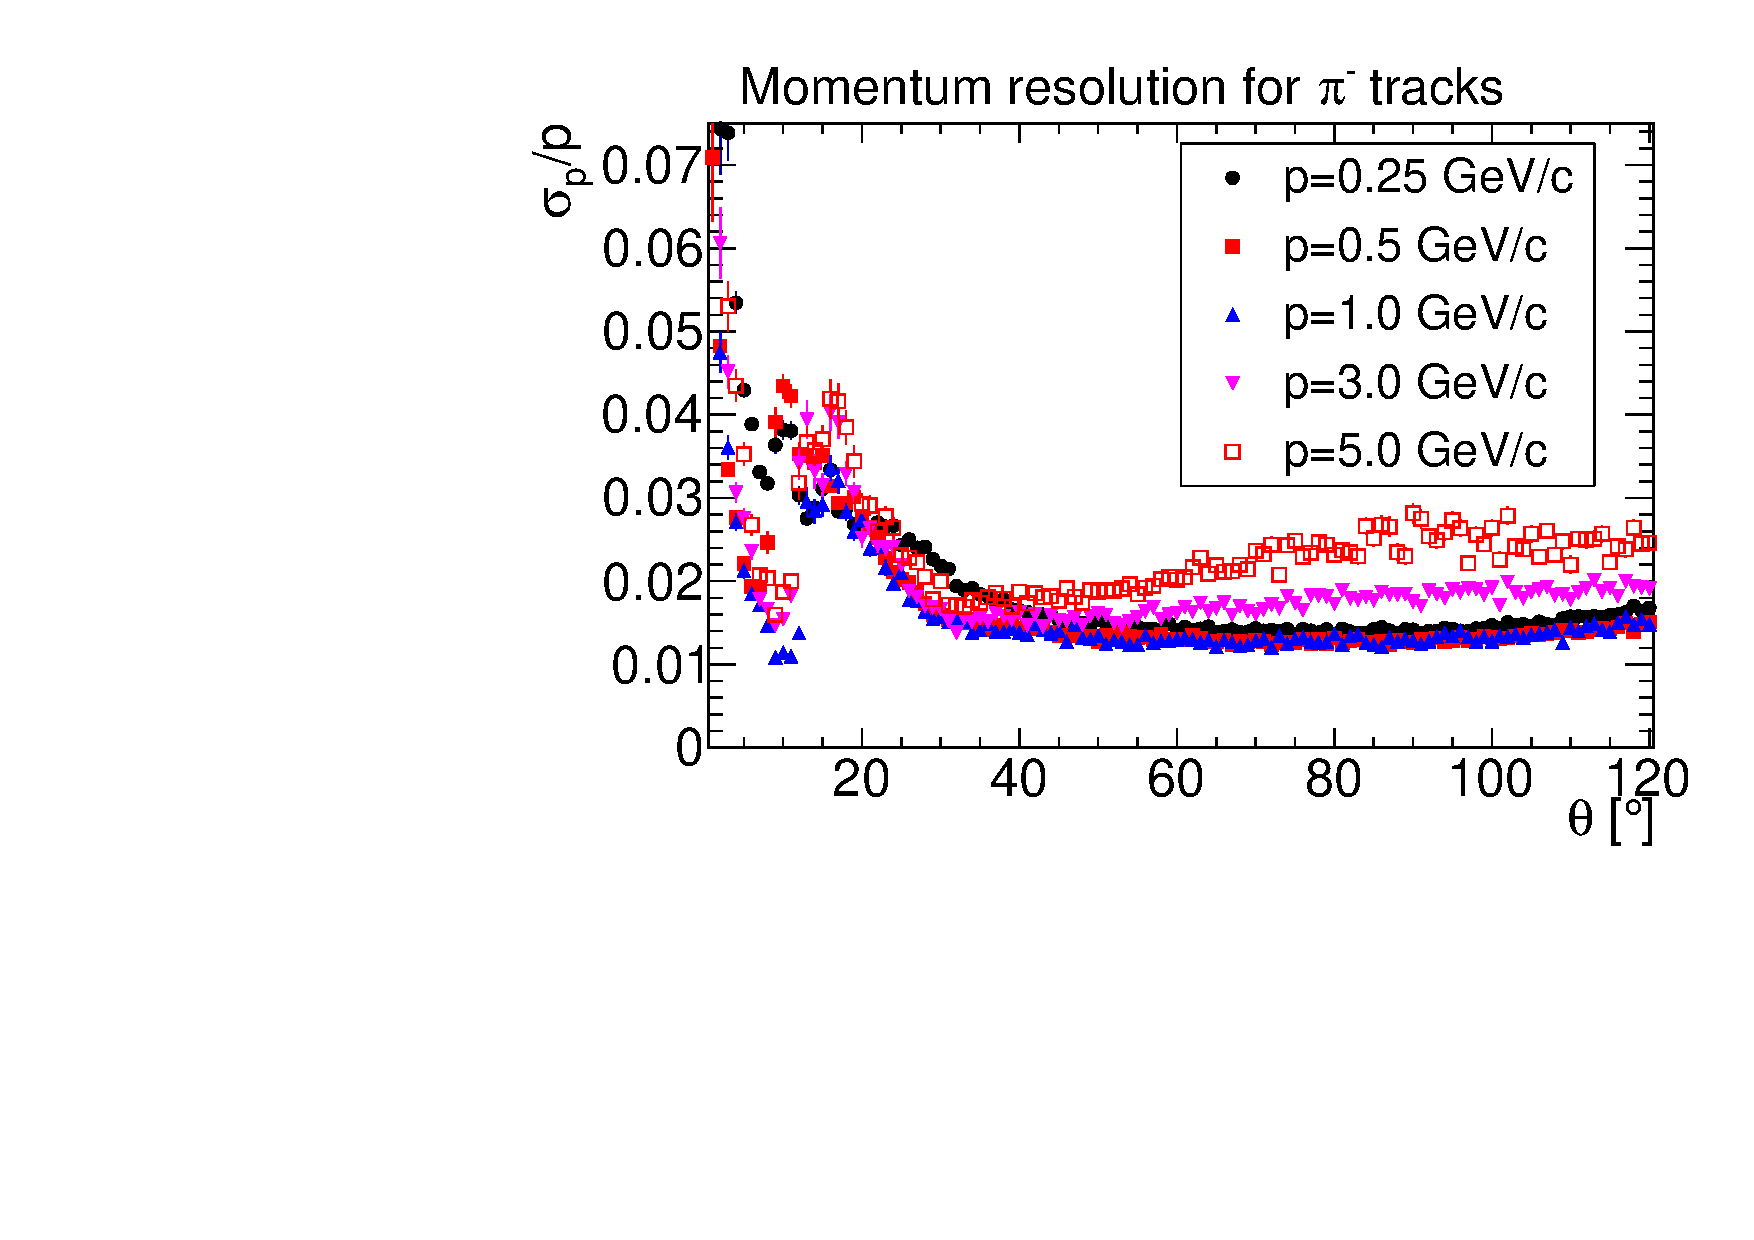
\includegraphics[width=0.45\textwidth]{figures/PionMomentumResolution.pdf}
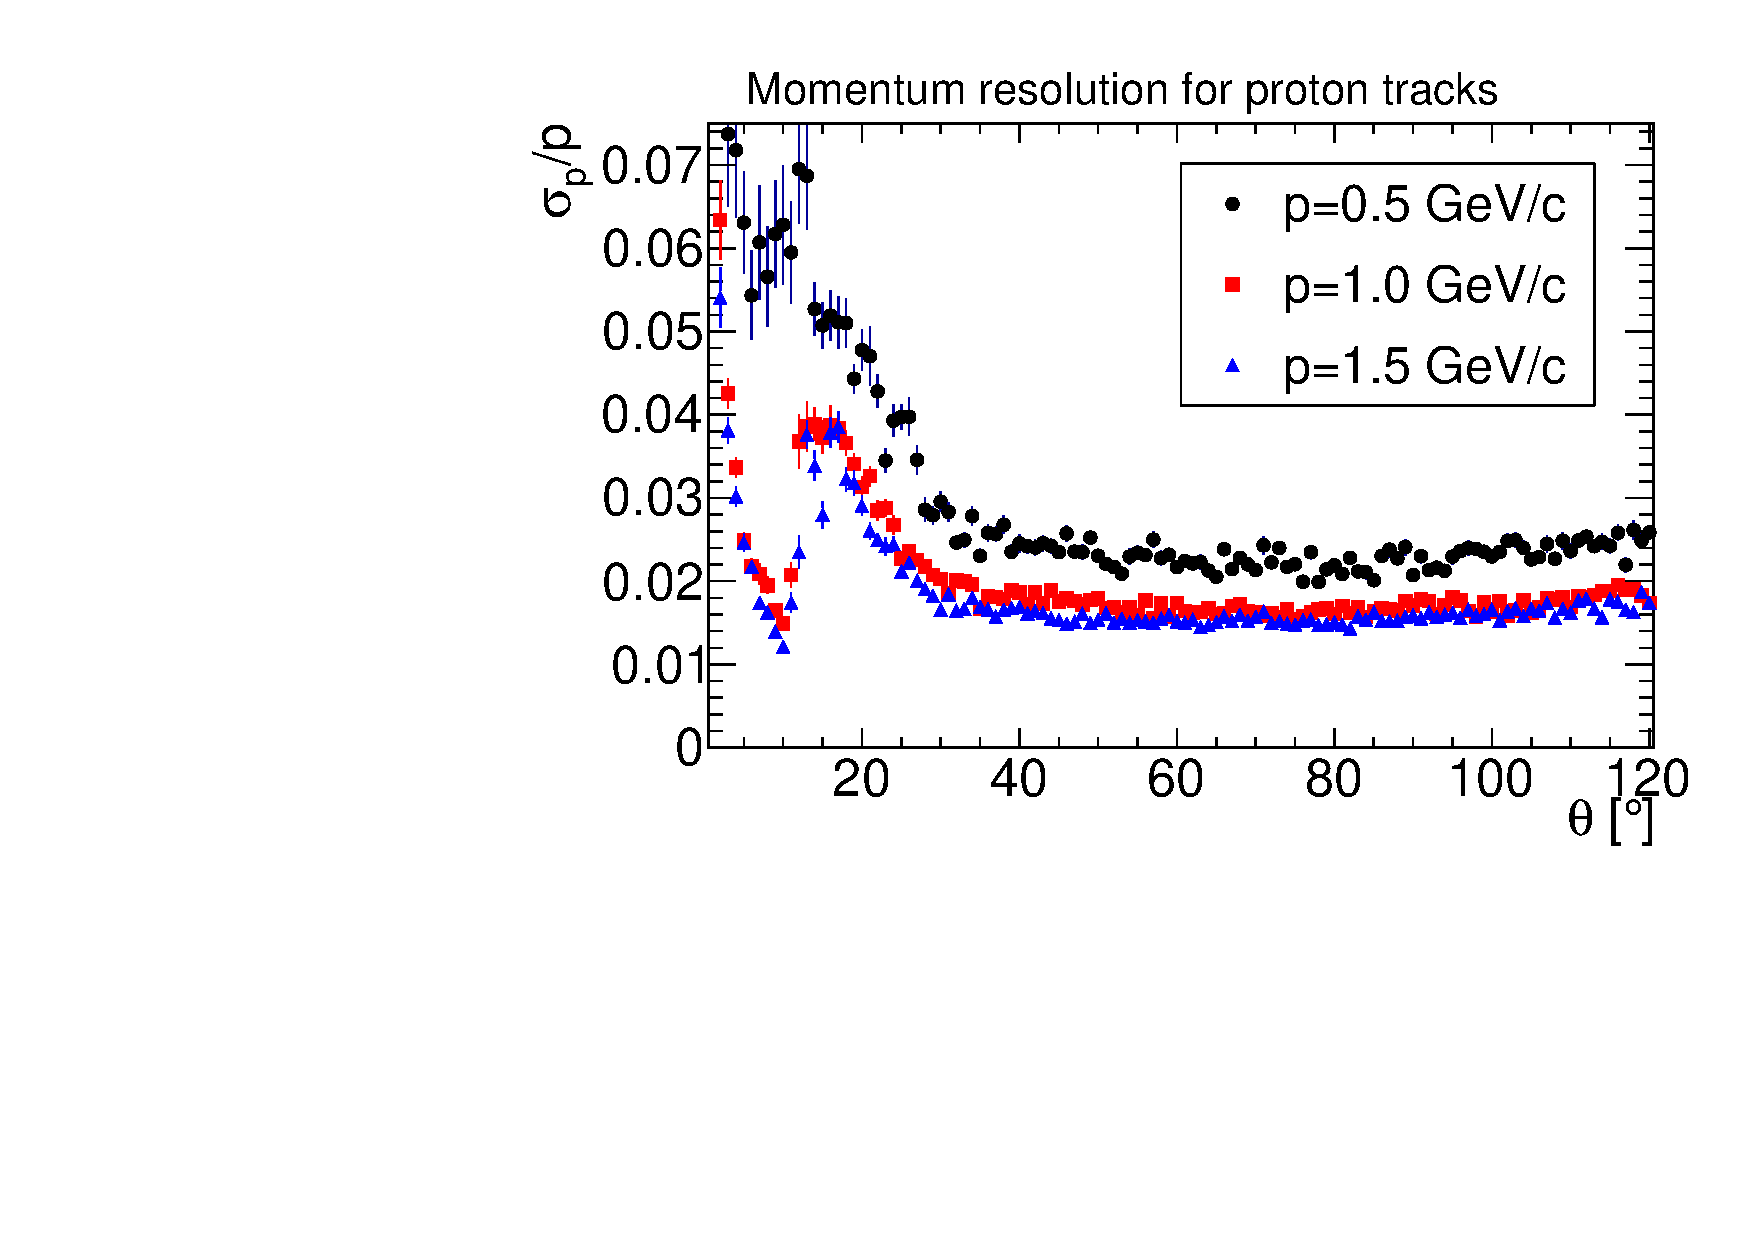
\includegraphics[width=0.45\textwidth]{figures/ProtonMomentumResolution.pdf}
\caption{\label{fig:dp_p} (Left) Momentum resolution for $\pi^-$ tracks.
(Right) Momentum resolution for proton tracks. (Color online)}
\end{center}
\end{figure}

\begin{figure}[tbp]
\begin{center}
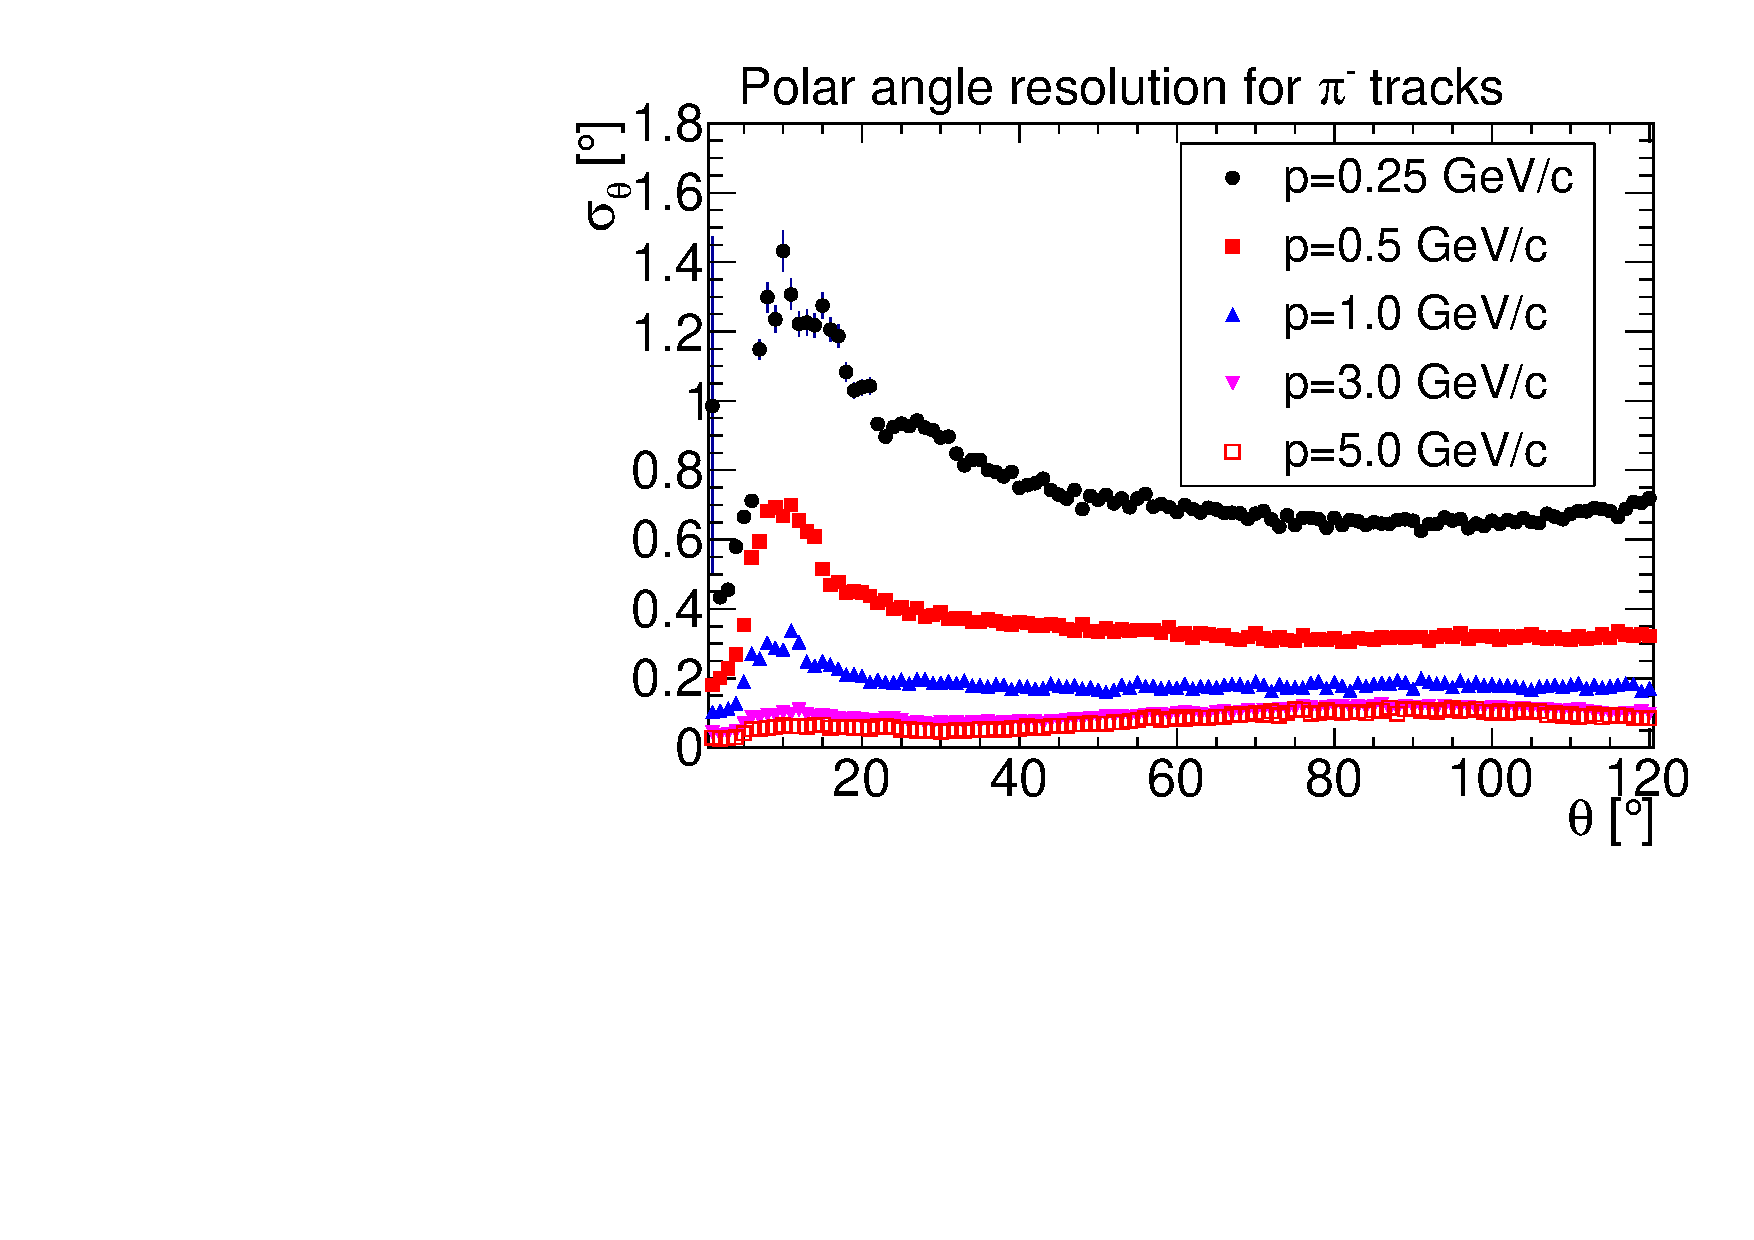
\includegraphics[width=0.45\textwidth]{figures/PionThetaResolution.pdf}
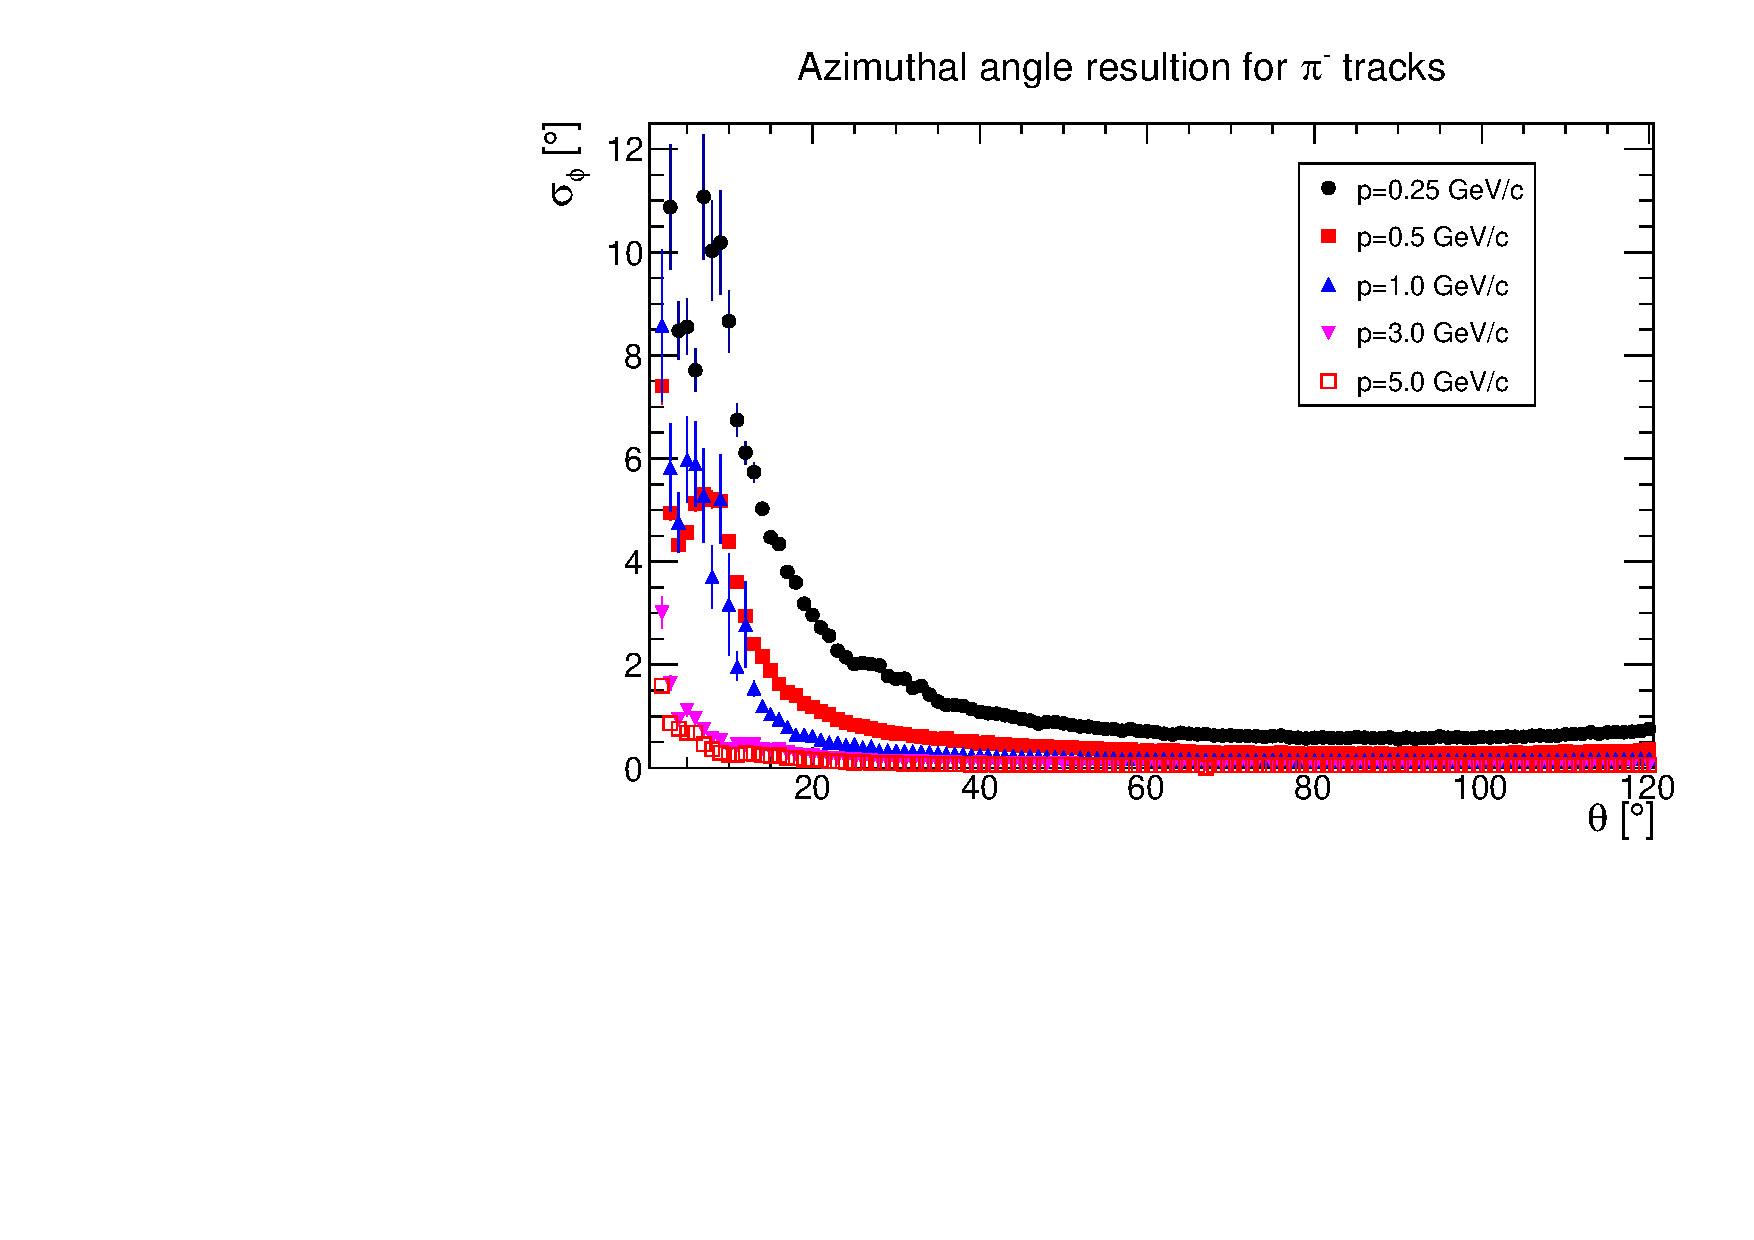
\includegraphics[width=0.45\textwidth]{figures/PionPhiResolution.pdf}
\caption{\label{fig:angle res} (Left) Polar angle resolution for $\pi^-$ tracks.
(Right) Azimuthal angle resolution for $\pi^-$ tracks.
 (Color online)}
\end{center}
\end{figure}


\subsection{Vertex resolution}

The thin windows of the cryogenic target and the exit window of the target
vacuum chamber provide a means to estimate the 
vertex resolution of the tracking system.  We use pairs of tracks from 
``empty target'' runs to reconstruct these windows as illustrated in 
Fig.~\ref{fig:z-vertex}.  We required $d<1$ cm, where $d$ is the 
distance-of-closest-approach between the two tracks. The ``vertex'' position 
is at the mid-point of the line segment of length $d$ connecting the two tracks.
The estimated z-position resolution is 3 mm.

\begin{figure}[tbp]
\begin{center}
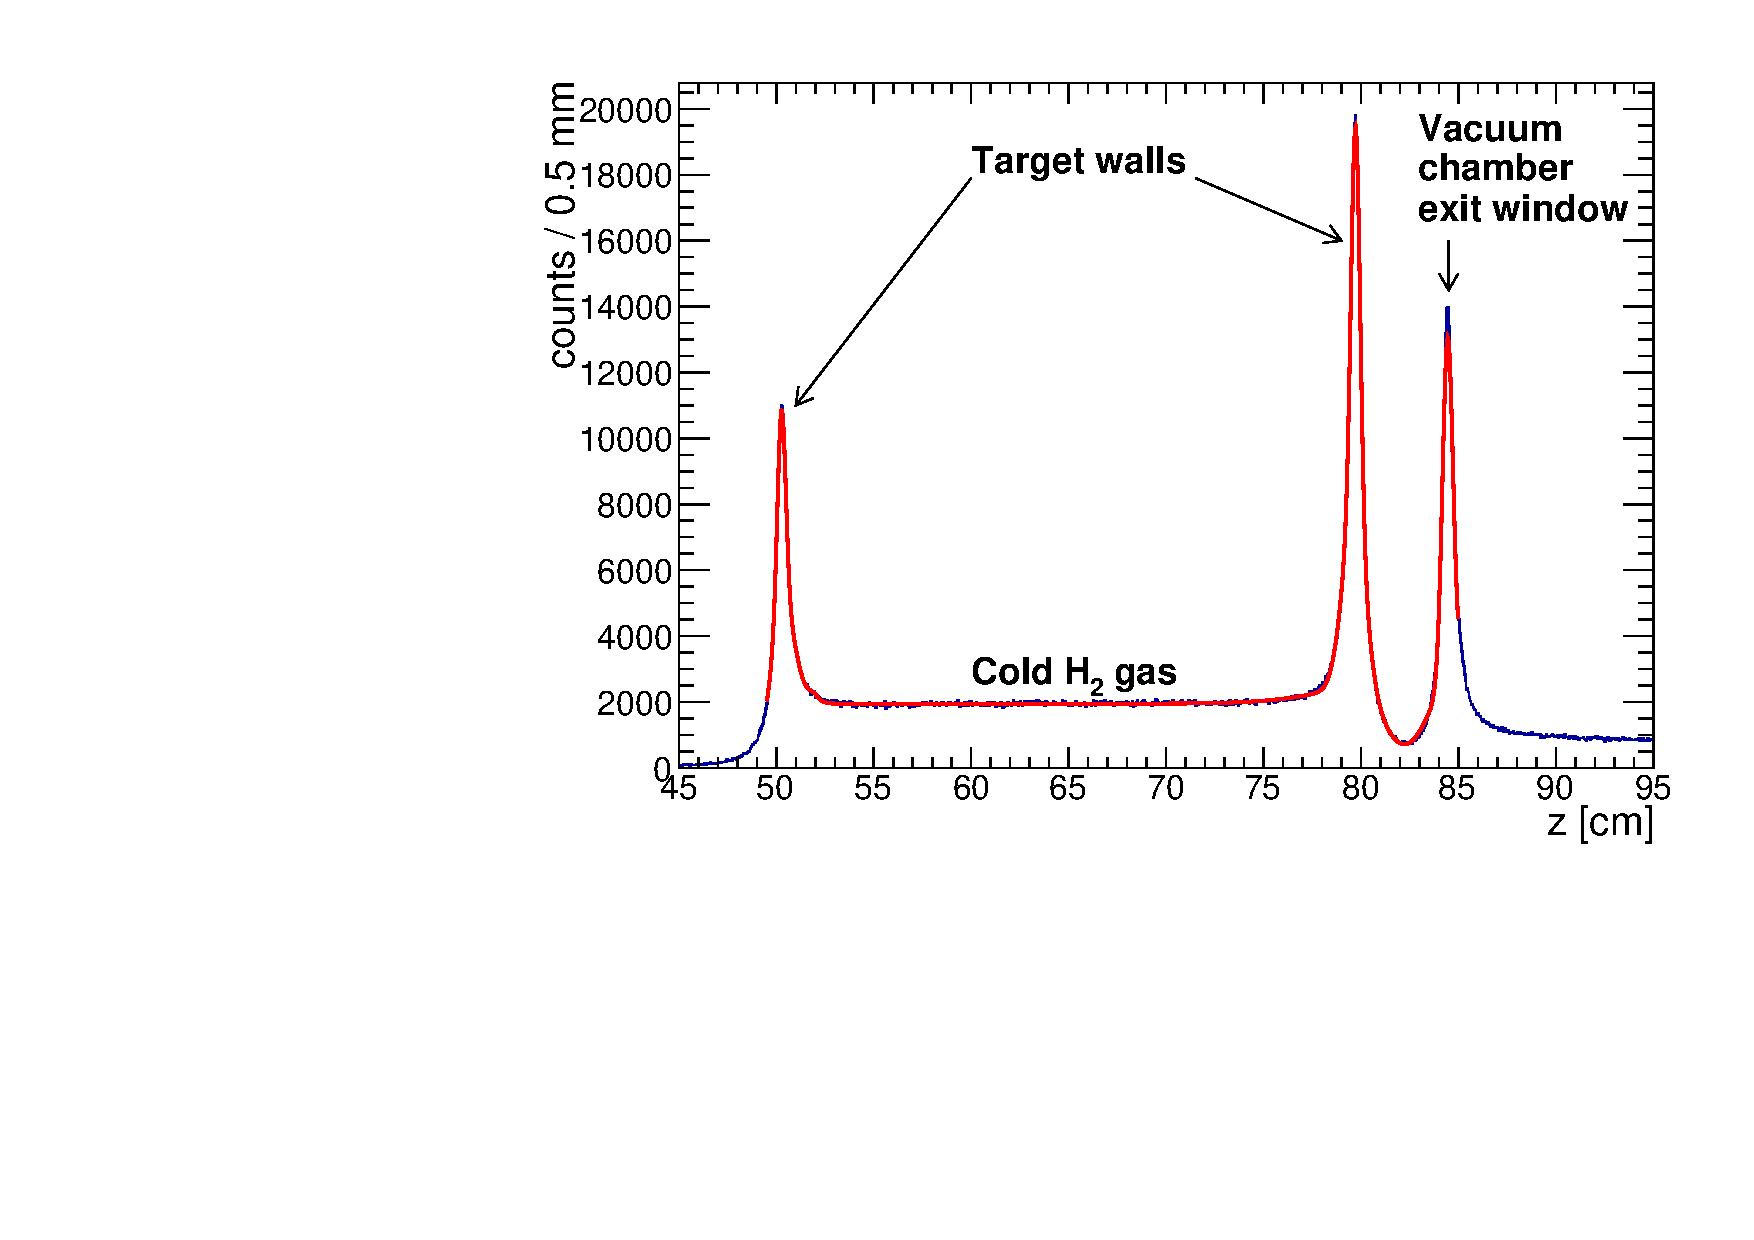
\includegraphics[width=0.7\textwidth]{figures/ZVertex.pdf}  
\caption{\label{fig:z-vertex} Reconstructed vertex positions within 1 cm radial
 distance with respect to the beam line for an empty target run.  The curve shows the result of a fit to the vertex distribution used to determine the vertex
resolution.  (Color online). 
}   
\end{center}  
\end{figure}


\section[Electromagnetic calorimeters] {Electromagnetic calorimeters \label{sec:calorimeters}}

\subsection[Barrel calorimeter ]{Barrel calorimeter \label{sec:bcal}}
The barrel calorimeter (BCAL) is an electromagnetic sampling calorimeter that detects photon showers with energies between 0.05~GeV and several GeV, $11^{\circ}$--$126^{\circ}$ in polar angle, and $0^{\circ}$--$360^{\circ}$ in azimuthal angle, which defines a geometry that is fairly unique among calorimeters. The containment of showers depends on the angle of photon incidence, with a thickness of $15.3$ radiation lengths for particles entering normal to the calorimeter face and reaching up to 67 radiation lengths at $14^{\circ}$. Details of the design, construction and performance of the BCAL can be found in Ref.\cite{BEATTIE201824}.

The BCAL is constructed as a lead and  scintillating-fiber matrix, consisting of 0.5~mm-thick corrugated lead sheets and 1.0~mm-diameter Kuraray SCSF-78MJ multi-clad fibers, the latter running parallel to the cylindrical axis of the detector. Each module has approximately 185 layers and 15,000 fibers. Geometrically, the BCAL consists of 48 optically isolated modules each with a trapezoidal cross section, forming a  390~cm-long cylindrical shell having inner and outer radii of 65~cm and 90~cm, respectively. The light generated in the fibers is collected via small light guides at each end of the module and transported to silicon photomultipliers (SiPMs), which were chosen due to their insensitivity to magnetic fields. The end of the calorimeter with light guides, light sensors and electronics is shown in  Fig.\,\ref{fig:bcal:bcal_assemblies}.

\begin{figure}[tbp]\centering
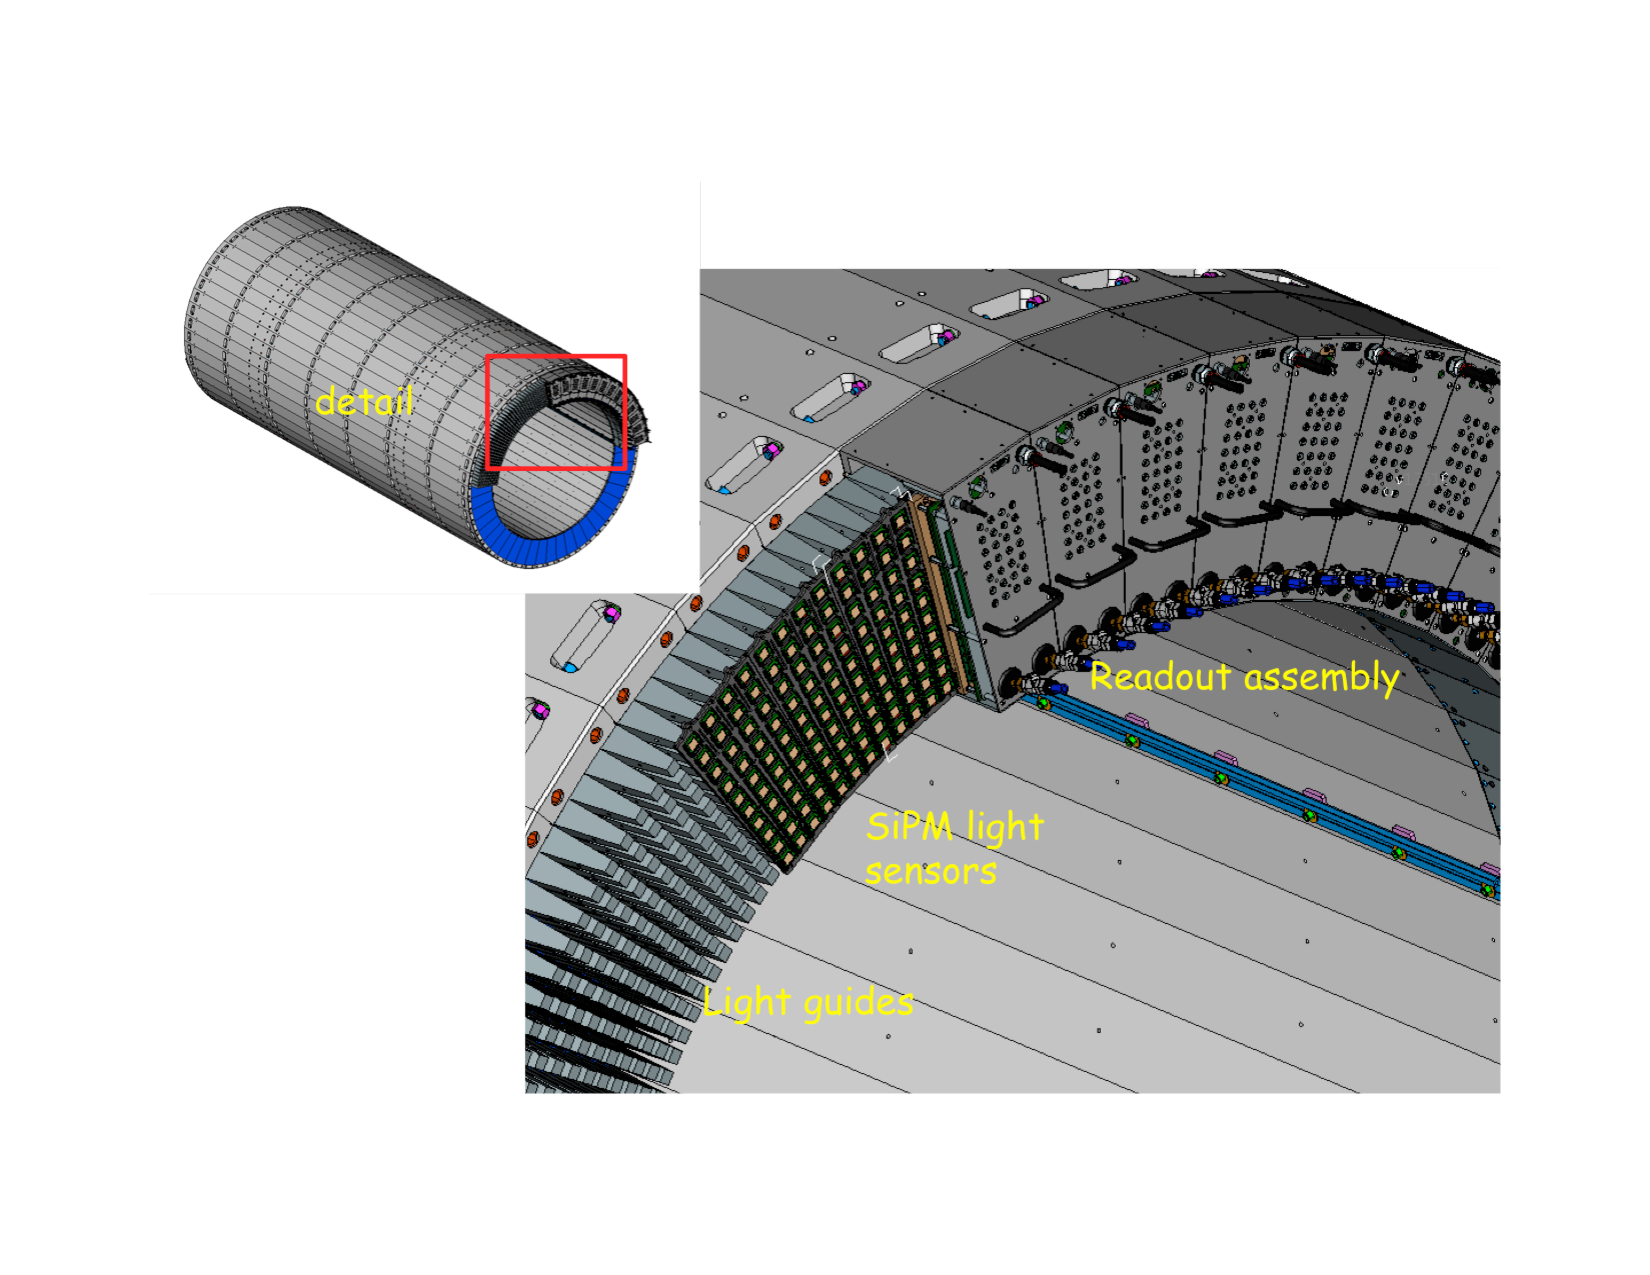
\includegraphics[scale=0.4]{figures/bcal_assemblies.pdf}
\caption{\label{fig:bcal:bcal_assemblies}
   Three-dimensional rendition of the light guides mounted at the end of the 
   BCAL, as well as the readout assemblies mounted over them. The 
   readout assemblies contain the 
   SiPMs and their electronics.  (Color online)
  }
\end{figure}


The SiPM light sensors are Hamamatsu S12045(X) Multi-Pixel Photon Counter (MPPC) arrays \footnote{Hamamatsu Corporation, Bridgewater, NJ 08807, USA \\ (\url{http://sales.hamamatsu.com/en/home.php)}.}, 
which are $4\times4$ arrays of $3\times3$ mm$^2$ tiles \cite{hdnote2913}. The SiPMs were tested extensively before acceptance \cite{Barbosa2012100,Qiang2013234,soto,Soto201489,BeattieIEEE,doi:10.1063/1.4955340}. Four thousand units were purchased and 3840 are installed in the detector. The gain of the SiPM depends on the voltage above the breakdown voltage, which is about 70~V. We operate them at 1.4~V over the breakdown voltage, which was selected to reduce the effect of readout thresholds. Even at this relatively high over-bias, the noise level is dominated by fluctuations in the electronics baseline and not by single-pixel noise. In order to keep a constant gain, we maintain the temperature within practical limits ($\pm$ 2$^\circ$C) using a chilled water system and then stabilize the gain using a custom circuit that adjusted the bias voltage based on the measured temperature. Two stages of preamplifiers and summing electronics are attached to the sensors. In order to reduce the number of signals that are digitized, circuits sum the outputs of the preamplifiers in groups of radial columns, with coarser granularity away from the target. The layer closest to the target employs a single SiPM, and the next three have 2, 3, and 4 SiPMs, respectively. On the end of each module, forty SiPMs generate sixteen signals that are delivered to flash ADCs (FADCs) and twelve signals that are discriminated and then recorded with pipeline TDCs. The FADCs and TDCs are conveniently located on the floor of the experimental hall in VXS crates.

\begin{figure}[tbp]\centering
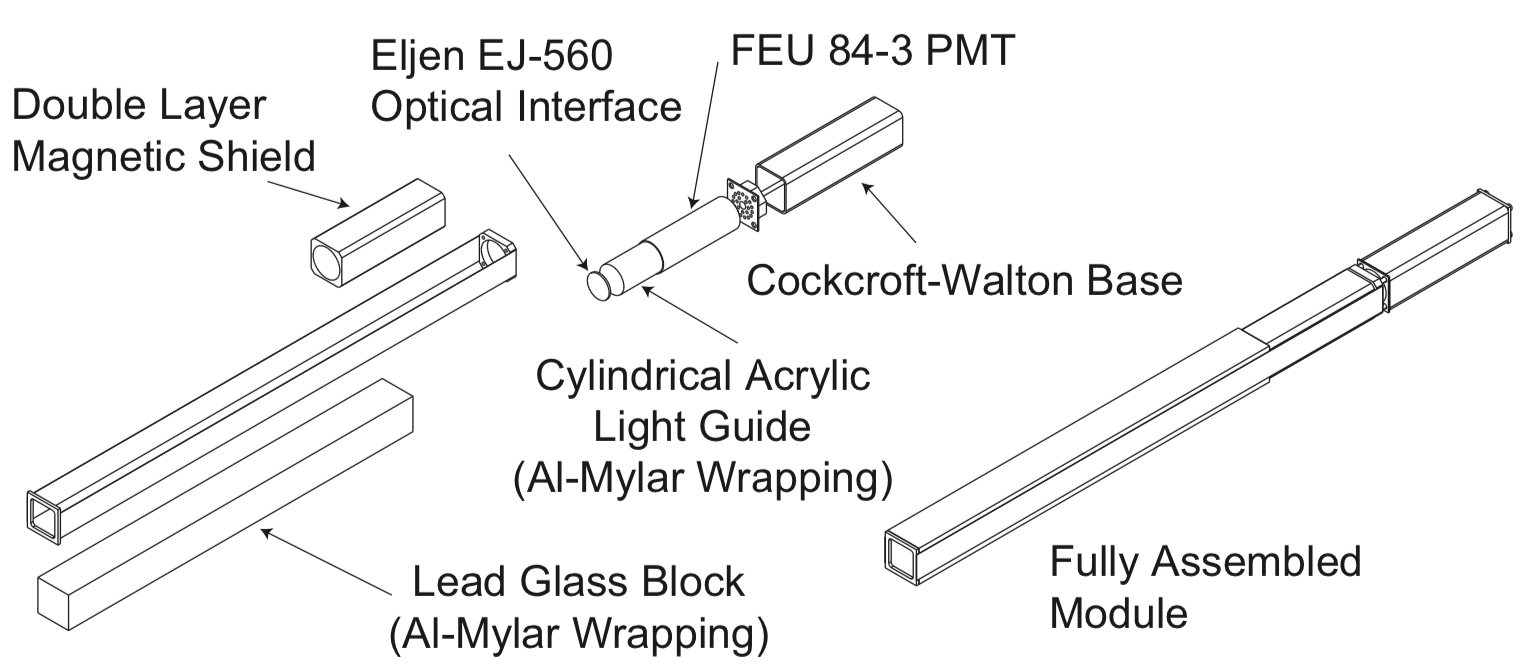
\includegraphics[height=5cm]{figures/FCAL_single_module}
\caption{\label{fig:fcal:FCAL_single_module}
    Expanded view of a single FCAL module.
  }
\end{figure} 
\subsection{Forward calorimeter \label{sec:fcal}}
The forward calorimeter (FCAL) detects photon showers with energies ranging from 0.1 GeV to several GeV, and  between $1^{\circ}$--$11^{\circ}$ in polar angle. The front face of the FCAL is located 5.6~m downstream from the center of the GlueX target and consists of 2800 lead glass blocks --- each having transverse dimensions $4\times4$ cm$^2$ and length of 45~cm ---  stacked in a circular array that has a diameter of 2.4~m.  The lead glass blocks are equivalent to type F8 manufactured by the Lytkarino Optical Glass Factory,\footnote{http://lzos.ru .}. The blocks and most of the PMTs are the same as those used in previous experiments: E852 at Brookhaven National Laboratory \cite{CRITTENDEN1997377} and the RadPhi Experiment at JLab \cite{JONES2007384}. To remove accumulated radiation damage, the glass was annealed by heat treatment prior to installation in GlueX. The detector is enclosed in a dark room.

The light collection from the lead-glass block into the PMT is accomplished, sequentially, via an Eljen EJ-560 optical interface ``cookie'' and a UVT acrylic cylindrical light guide glued to the PMT. The light guide recesses the magnetically sensitive photocathode of the PMT inside a dual layer of soft iron and mu-metal that attenuates the stray field of the GlueX solenoid of up to 200~G. The sensors are FEU 84-3 PMTs with Cockcroft-Walton bases, each consuming 0.2~W of power.  The design of the PMT base is similar to that noted in Ref.~\cite{Brunner:1998fh} and eliminates the need for a 2800-channel high-voltage power system. The bases communicate with a controller utilizing the CAN protocol \cite{wiki:CANBus}, with 100 bases on each of 28 CAN buses.  The communication allows continuous monitoring of the PMT voltages, temperatures, and current draw.
A schematic of a single FCAL module is shown in 
Fig.\,\ref{fig:fcal:FCAL_single_module} and more details may be found in Ref.\,\cite{MORIYA201360}. FCAL signals are routed to FADC electronics, situated on a platform, directly behind the FCAL dark room.

\subsection{Electronics \label{sec:calelectronics}}
Custom readout electronics for the two calorimeters are mounted in standard VXS crates and include 
JLab 12-bit 250~MHz FADCs \cite{hdnote1022}, discriminators \cite{hdnote2511} and F1 Time-to-Digital Converters (TDCs) \cite{hdnote1021}. The maximum input scale of the FADCs (4095 counts) is set to 2~V.
The FADCs sample each calorimeter channel every 4~ns and generate raw waveforms consisting of 100 samples 
 (400~ns), which are available for further processing by the firmware upon a trigger signal if there is a threshold crossing. The firmware computes several derived features of the pulse: pedestal, peak value, integral over a selected window, and time of the half-way point on the leading edge. At most one pulse is extracted from each readout window. These pulse features constitute the raw data that is nominally read out from the FADC.  Optionally, the full waveforms can be read out for diagnostic purposes and to check the firmware output against the offline emulation of the parameter extraction; this is done for less than about 1\% of the production runs.
 
We describe the feature extraction of pulses in more detail.
Pulses are identified by the first sample that exceeds a threshold, currently set to 5 (8) counts above the average pedestal for the BCAL (FCAL). These thresholds correspond to approximately 2.5 (12) MeV for the BCAL (FCAL). The integral is determined using a fixed number of samples relative to the threshold crossing, which was determined by maximizing the ratio of signal to pedestal noise.  The integration window begins one sample before the threshold time and extends to 26 (15) samples after the threshold time for the BCAL (FCAL).  Typical pedestal widths are $\sigma\sim$1.2-1.3 (0.8) counts for the BCAL (FCAL).  For the BCAL, the pedestals are determined for each channel event-by-event, appropriately scaled, and then subtracted from the peak and integral to obtain signals proportional to the energy deposited in the calorimeter, while for the FCAL, the average pedestal over a run period is determined offline for each channel and its contribution to the pulse integral is subtracted when the data are reconstructed.  %See Fig.\,\ref{fig:Plot_waveform10}.  
 The algorithm that determines the time of the pulse is pulse-height independent and therefore no time-walk correction is required for the FADC times~\cite{Bennett:2010nf}.

The outputs of the three inner layers of the BCAL are also connected to leading-edge discriminators, which feed the JLab F1 TDCs. The discriminator thresholds are typically set to about 35~mV, but are adjusted
 channel by channel.  The pulse times are recorded relative to the trigger in a 12-bit word. Multiple hits may be recorded per channel per event (up to eight), but are culled at a later time by comparison to FADC times. The nominal least count is configured to 58~ps.


\subsection[Calibration and monitoring]{Calibration and monitoring \label{sec:calcalib}}
The relative gains of the calorimeters are monitored using a modular LED-driver system \cite{Anassontzis201441}. The control system is the same for both calorimeters, but the arrangement of LEDs is tailored to the geometry of each detector. In the BCAL, there is one LED inserted into each light guide, which can be used to monitor each individual SiPM and its partner at the far end of the module.
Due to geometry the illumination varies considerably from channel to channel. 
The average stability of the detector over a period of ten days is better than 1\% and the fractional root-mean-square (RMS) deviations of the mean for each SiPM during a single day from the average over the run period is typically less than 2\%.

For the FCAL, we installed four acrylic panes, each covering the upstream end of one quadrant of the FCAL. Each pane is illuminated by forty LEDs, ten violet, ten blue and twenty green. In addition to monitoring the stability of the readout, the different colors are used to study the wavelength dependence of the transmission of light though the lead glass blocks.  In particular, radiation damage to lead glass inhibits transmission at the blue end of the spectrum and tends to turn glass a brownish color~\cite{Schaefer:2011gw}.  Throughout a several-month run, in the blocks closest to the beam line, the PMT response to violet LED degraded by about 10\% while the response to the green LED was unchanged, characteristic of radiation damage.  Such damage is only evident in the first two layers of blocks surrounding the 12~cm$\times$12~cm beam hole. This damage is likely confined to the upstream end of the block and does not significantly affect the response to particle showers in the body of the glass.

The energies of photons impinging on a calorimeter are obtained by ``clustering'' or grouping together hits that are close in time and space. Details of the algorithms to obtain shower energies in the BCAL can be found in Ref.\,\cite{BEATTIE201824}  and in Ref.\,\cite{Jones:2006ru} for the FCAL. The clustering in the FCAL requires that hits come within 15 ns of the primary hit and the seed threshold is taken to be 35 MeV, and showers with a single hit are discarded. In the event of overlapping showers, the hit energies are divided amongst the clusters in proportion to that predicted by a typical shower profile. Both detectors have sources of energy-dependent nonlinearities and empirical corrections are developed and applied to minimize the measured energy dependence of the measured $\pi^0$ mass.  


\subsection{Performance \label{sec:calperformance}}
The performance of the calorimeter is summarized by its ability to measure the energy, position and timing of electromagnetic showers.

The energy resolution of each calorimeter was extracted from the measured $\pi^0$ and $\eta$ mass distributions, which yielded consistent results. 
To study the $\eta$ mass resolution, we selected events using kinematic fits to $\gamma p \rightarrow p \pi^+ \pi^- \gamma \gamma$, with $\eta\rightarrow \gamma\gamma$ and the photons having energies within 10\%.
The proton and pion tracks were used to determine the event vertex, needed to accurately reconstruct the two-photon invariant mass.
This reaction provides a fairly clean sample of $\eta$'s with energy ``symmetric" photons recorded either both in the BCAL or both in the FCAL. 
The single-photon energy resolution was determined from Gaussian fits to the $\eta$ invariant mass width, neglecting contributions from uncertainty in the opening angle.
Monte Carlo simulation of $\gamma p \rightarrow p \pi^+ \pi^- \eta$ events, with kinematics chosen to approximate the experimental distributions, were used to tune the MC resolution to match the data. 
The single-photon resolutions are shown in Fig.\,\ref{fig:bcal:eta_resolution}\,a) for the BCAL and Fig.\,\ref{fig:bcal:eta_resolution}\,b) for the FCAL as a function of the mean photon energy, both for data and simulation.
A fit has been performed to the data for each calorimeter to estimate contributions to noise from stochastic and constant processes.  The parameters in the fit are correlated due to the limited range in energy available for this data.

The resolution of the Z position in the BCAL ($\sim$\,2.5 cm) is computed from the timing resolution of the system, which was measured to be $\sigma=150$\,ps at 1\,GeV. The transverse position resolution for charged hadrons in the FCAL is $\sigma<$5~cm. 

The performance of the calorimeters has been demonstrated in the reconstruction of neutral states including $\pi^0$, $\eta$ and $\eta'$ mesons for the first \gx{} physics publications \cite{AlGhoul:2017nbp,Adhikari:2019gfa}. In addition, although the response of the calorimeters at high-energy is still under evaluation, they have provided important electron-pion separation in order to identify the decays of $J/\psi\rightarrow e^+e^-$ \cite{Ali:2019lzf} where electrons are recorded up to 8~GeV. 

\begin{figure}[tbh]\centering
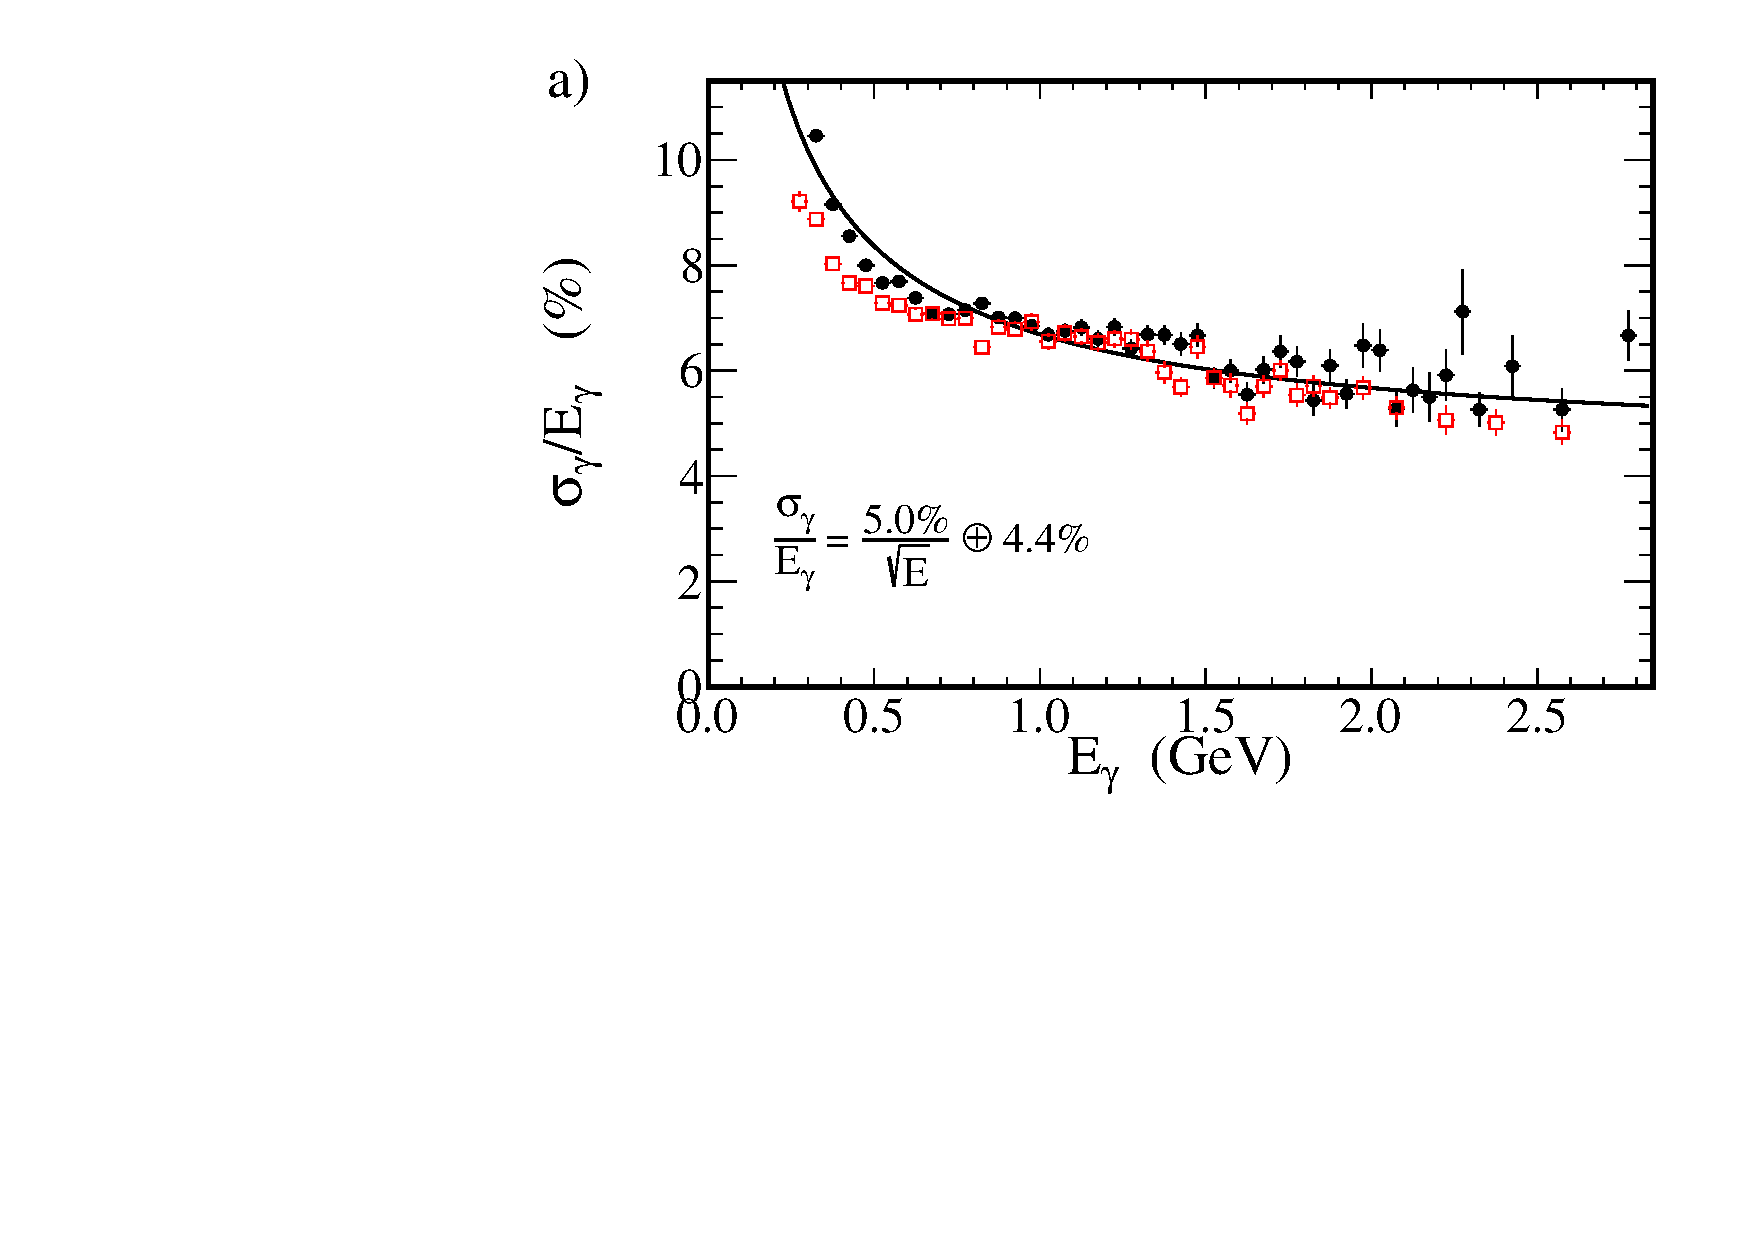
\includegraphics[width=0.48\textwidth]{figures/fit_BCAL_energy_resolution_sigma.pdf} 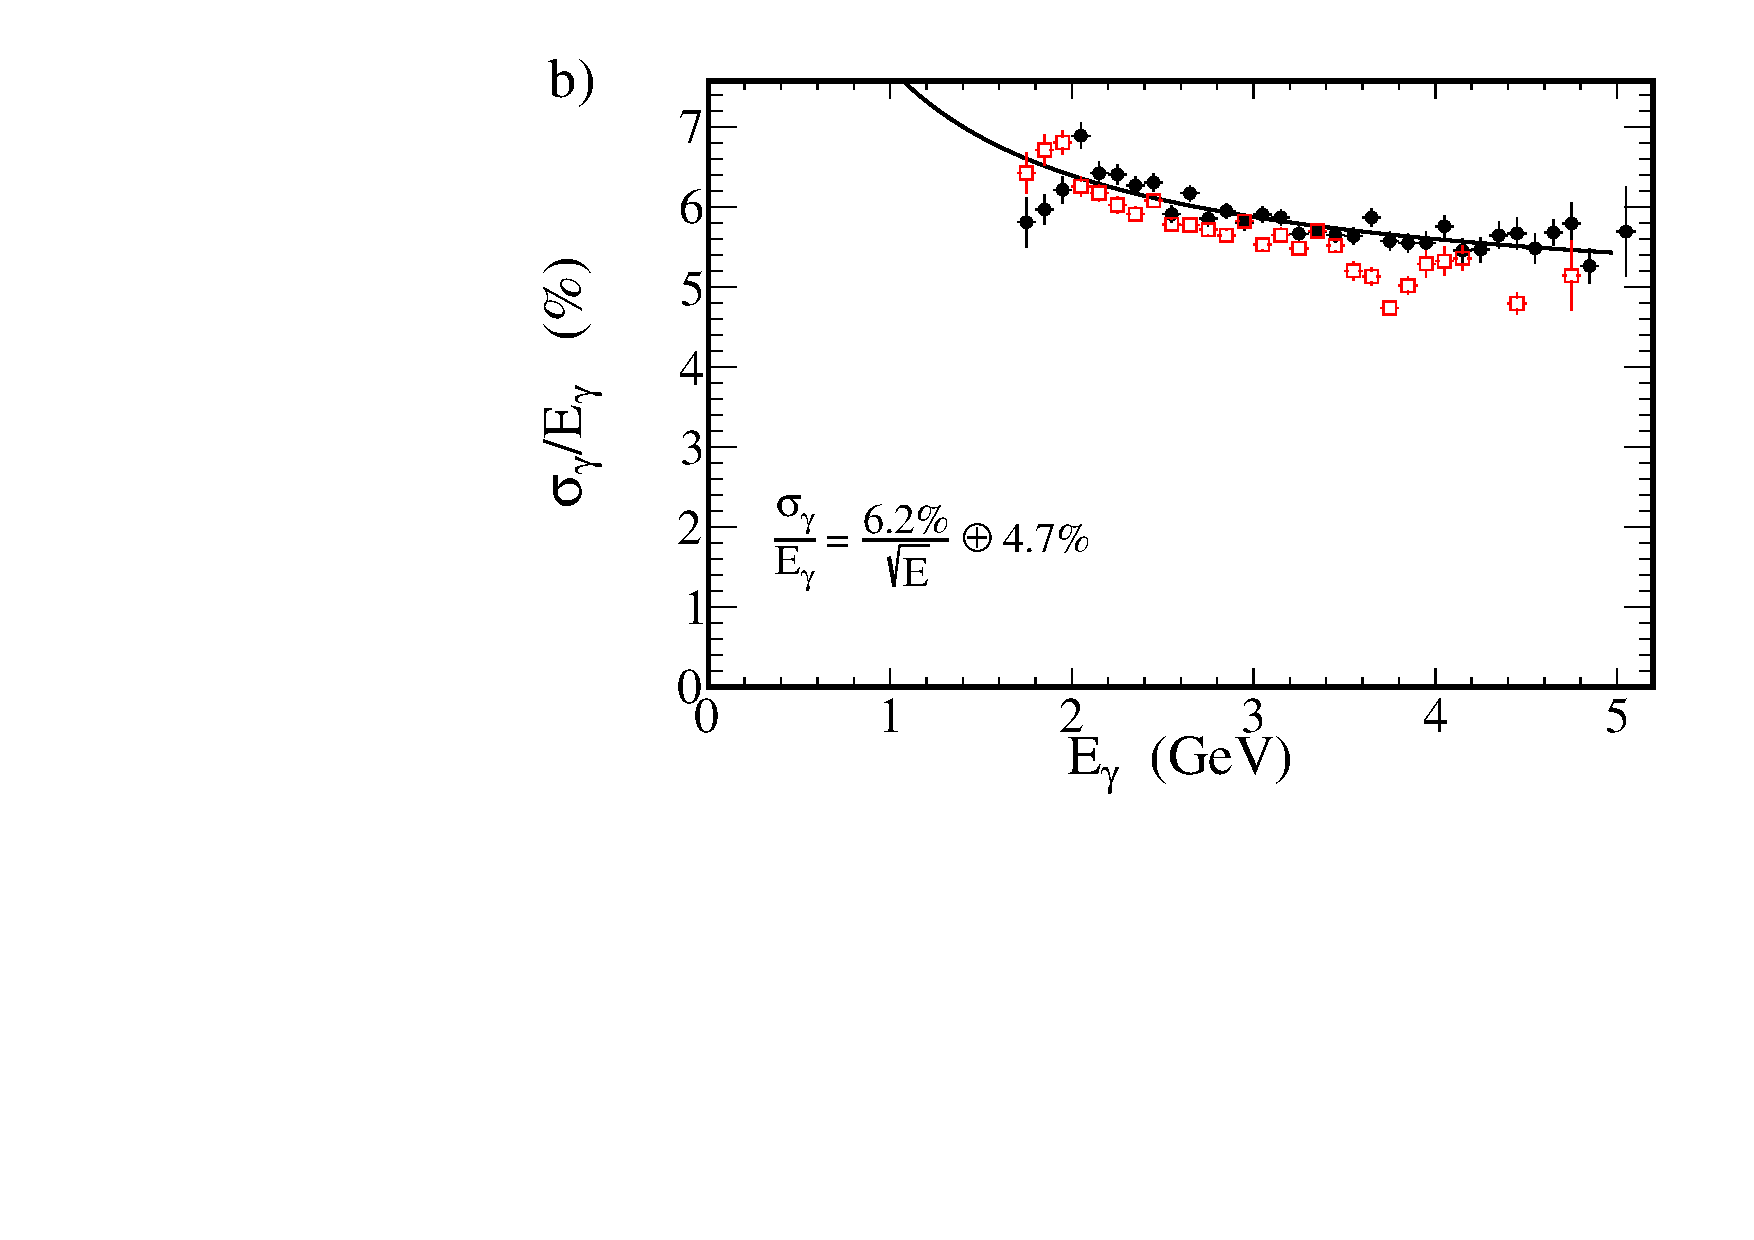
\includegraphics[width=0.48\textwidth]{figures/fit_FCAL_energy_resolution_sigma.pdf}
\caption{\label{fig:bcal:eta_resolution} 
The energy resolution of single photons in the a) BCAL and b) FCAL calculated from the $\eta$ mass distribution under the assumption that only the energy resolution contributes to its width.  Solid black circles are data and open red squares are simulation.
(Color online)
 }
\end{figure}    


%\subsection{Summary \label{sec:calsummary}}
\clearpage    % avoid formatting problems with empty sections
\section[Scintillation detectors (Mark I./Beni)]{Scintillation detectors \label{sec:scintillators}}
\subsection{Start counter \label{sec:st}}
\subsection[Time-of-flight counters (Beni)]{Time-of-flight counters \label{sec:tof}}
\subsection{Electronics \label{sec:scelectronics}}
\subsection{Calibration and monitoring \label{sec:sccalib}}
\subsection{Performance \label{sec:scperformance}}
\subsection{Summary \label{sec:scsummary}}

%=======================+=========================
%==============  Trigger    ================
%=================================================\

\section{Trigger (Sasha) \label{sec:trig}}
\subsection{Architecture \label{sec:trigarchitecture}}
The goal of the GlueX trigger is to accept most high-energy hadronic interactions while reducing the background rate induced by electromagnetic and low-energy hadronic interactions leading to an overall rate of about 80 kHz, which is acceptable by the DAQ.  The trigger system of the GlueX experiment\cite{GlueX:2013twa} is implemented on pipelined special-purpose programmable electronics modules with Field-Programmable Gate Array (FPGA) chips. The modules were designed at Jefferson Lab.  The GlueX trigger and read out electronics is hosted in VXS (ANSI/VITA 41.0) crates; VXS is an extension of the VME/VME64x architecture, that implements high-speed backplane lines used to transmit trigger information. The main trigger algorithm is 
based on measurement of the energy depositions in two electromagnetic calorimeters~\cite{somov_l1}. Supplementary triggers can also
use hits from scintillator detectors, such as the PS, tagging detectors, ST, and TOF.

A layout of the trigger system is presented in Fig.~\ref{fig:trig}. Data from the Forward and Barrel calorimeters are sent to  Flash ADC (FADC250)~\cite{Dong:2007} modules, situated in 12 and 8 VXS crates, respectively, and are digitized at the sampling rate of 250 MHz. The digitized amplitudes are used for the trigger and are also stored in the FADC FPGA-based pipeline for the subsequent readout via VME.
Digitized amplitudes are summed for all 16 FADC250 channels in each 4 ns sampling interval and are transmitted to the crate trigger processor (CTP) module, which sums up amplitudes from all FADC boards in the crate. The sub-system processor (SSP) modules located in the global trigger crate receives amplitudes from all crates and computes the total energy deposited in the FCAL and BCAL. The global trigger processor (GTP) module collects data from the SSPs, performs computation of different trigger equations and makes the trigger decision. The core of the trigger system is the trigger supervisor (TS) module. It receives the trigger information from the GTP and distributes triggers to electronics modules in all readout 
crates in order to initiate the data readout. There are 55 VXS crates in total in GlueX (26 with FADC250s, 14 with  FADC125s, 14 with F1 TDCs, and 1 CAEN TDC). The TS also provides a synchronization of all crates and sends a 250 MHz clock signal. The triggers and clock are distributed through the trigger distribution (TD) module in the trigger distribution crate and the trigger interface (TI) module and signal distribution (SD) module in each readout crate. The GlueX trigger system provides a fixed latency of about 3.1 $\mu$s.

\begin{figure}[tbp]
\begin{center}
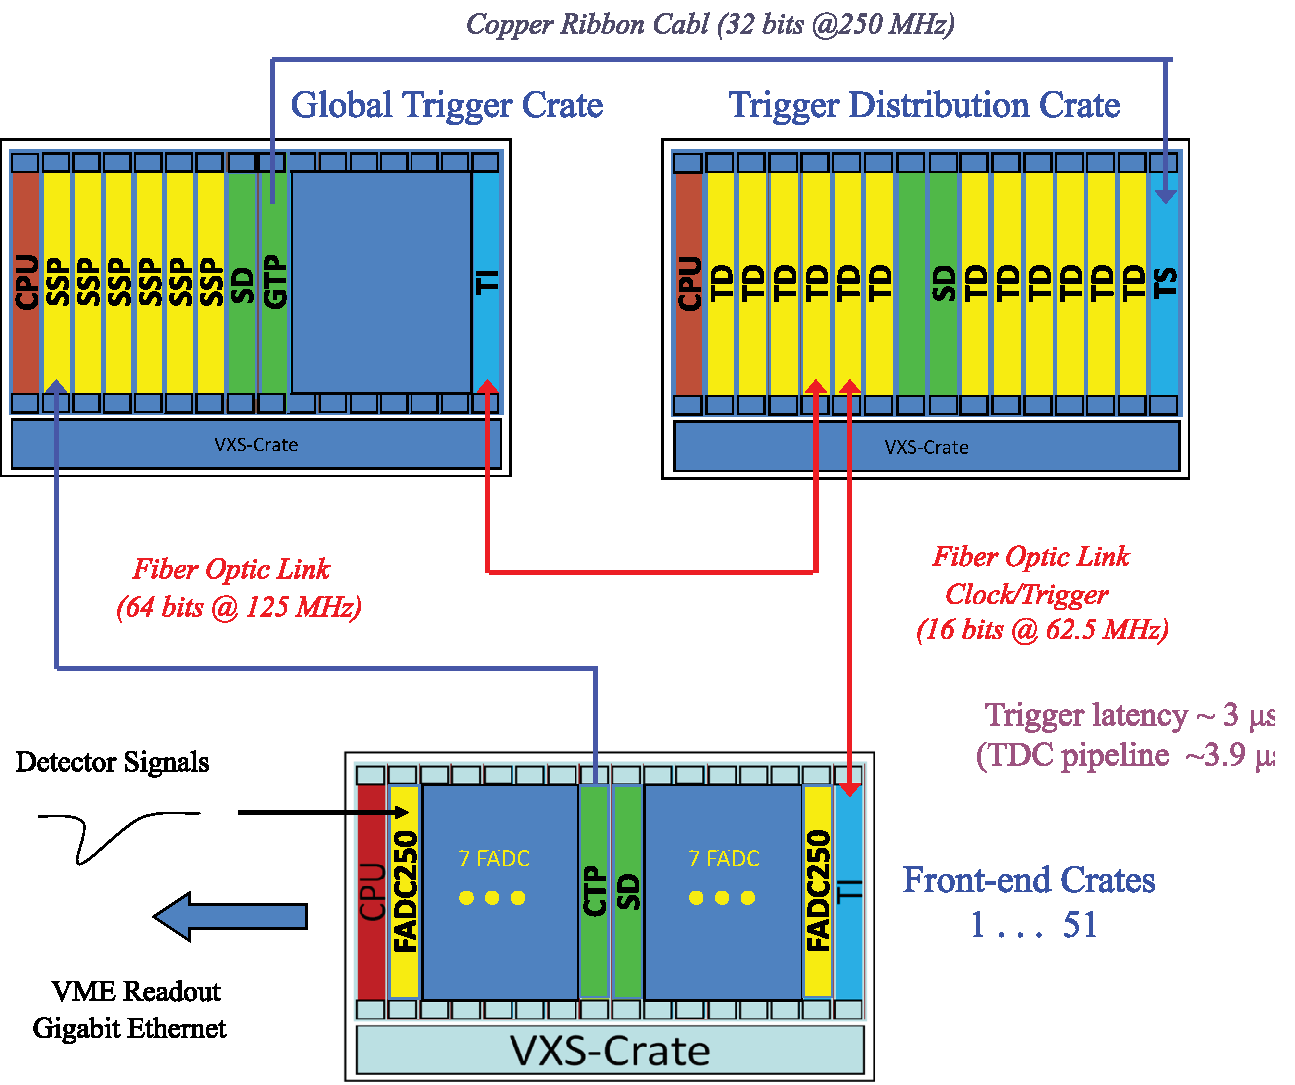
\includegraphics[width=0.75\textwidth]{figures/125_Somov-f1.pdf}  
\caption{Schematic view of the Level-1 trigger system of the GlueX experiment. Description of the electronics boards is given in the text.} \label{fig:trig}
\end{center}
\end{figure}

\subsection{Trigger Types \label{sec:triggers}}

The GlueX experiment uses two main trigger types: the pair spectrometer trigger, and the physics trigger based on energy depositions in the BCAL and FCAL. The 
pair spectrometer trigger is used to measure the flux of beam photons. This trigger requires a time coincidence of hits in the 
two arms of the PS detector, which is described in Section~\ref{sec:ps}. The physics triggers are generated when the FCAL and BCAL energies  satisfy the following equations (1) $2\cdot E_{\rm FCAL} + E_{\rm BCAL} > 1\;{\rm GeV}$,  $E_{\rm FCAL} > 0\; {\rm GeV}$ and (2) $E_{\rm BCAL} > 1.2\;{\rm GeV}$. The latter trigger type is used to accept events with large transverse energy released in the BCAL, such as decays of $J/\psi$ mesons.
Several other trigger types were implemented for efficiency studies and detector calibration. Ancillary minimum-bias random trigger, 
and calorimeter LED triggers were used concurrently with data taking. The rate of the random trigger and each of the LED triggers constituted 100 Hz and 10 Hz, respectively.

\subsection{Performance \label{sec:trigperformance}}
The rate of the main physics triggers as a function of the pair 
spectrometer trigger rate is shown in Fig.~\ref{fig:trig_rate}.
The typical rate of the PS trigger in the spring of 2018 was 3.5 kHz, which corresponds to a photon beam flux of about $2.5\cdot 10^7\; \gamma/{\rm sec}$ in the GlueX energy range of interest. The total trigger rate was about 40 kHz. The electronics and DAQ were running with the live time close to 
$100 \%$, collecting data from the GlueX detector at a rate of 600 megabytes per second.

%In spring 2018, data were collected at the luminosity %corresponding to the photon beam flux of about $2.5\cdot 10^7\; %\gamma/{\rm sec}$ in the GlueX energy range of interest. The %typical rate of the PS trigger 

\begin{figure}[tbp]
\begin{center}
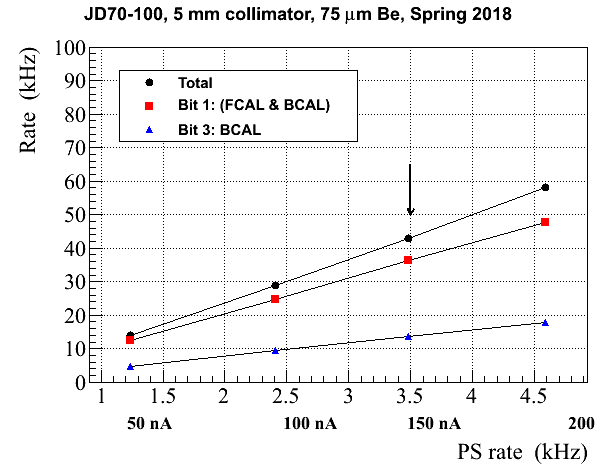
\includegraphics[width=0.75\textwidth]{figures/Rate_diamond_2018.png}  
\caption{Rate of the main production triggers as a function of the PS rate: FCAL \& BCAL trigger (boxes), BCAL trigger (triangles), the total trigger rate (circles). The vertical arrow indicates the run condition corresponding to the spring run of 2018.} \label{fig:trig_rate}
\end{center}
\end{figure}

%=======================+=========================
%==============  DAQ   ================
%=================================================\

\section[Data Acquisition]{Data acquisition \label{sec:daq}}

%\subsection{Architecture \label{sec:daqarchitecture}}

%\subsection{Performance \label{sec:daqperformance}}

The GlueX data acquisition uses the CEBAF Data Acquisition (CODA) framework. CODA is a software toolkit of applications and libraries that allows one to build customized data acquisition systems based on distributed commercial networks. A detailed description of CODA software and hardware can be found in Ref.\,\cite{CLAS12_DAQ}. 
The electronics in the VME/VXS crate can produce data up to 200 MB/s per crate and the
number of crates producing data is about 55.
The data from the electronic modules are read via the VME back-plane (2eSST, parallel bus) by the crate readout controller (ROC), which is a single board computer running Linux.
The \gx~ network layout and data flow are shown on Fig.~\ref{fig:CODA}.
Typical data rates from a single crate are in the range of 10--70~MB/s, depending on the detector type and trigger rate.
The ROC transfers data over 1~Gbit Ethernet link to Data Concentrators (DC) 40 event fragments at a time. Data Concentrators are programs, which build partial events received from 10-12 crates and run on a dedicated computer node.
The DC output traffic of 200-600 MB/s is routed to the Event Builder (EB) to build complete events.
The Event Recorder (ER), which is typically running on the same node as an event builder, write data to the local data storage.
To date, GlueX data has collected at a rate of 500--900 MB/s, which allows the ER to write out to a single output stream. The system is expandable to handle higher luminosity with rates of 1.5--2.5~GB/s. In this case, the ER must write multi-stream data to several files in parallel.
All DAQ nodes {\color{red} Elton: nodes same as CPUs / ROCs? } are connected to both a 40 Gb Ethernet switch and a 56 Gb Infiniband switch.
The ethernet network is used exclusively for DAQ purposes: receiving data from detectors, building events, and writing data to disk, 
while the Infiniband network is used to transfer events for online data quality monitoring. 
This allows one to decouple DAQ and monitoring network traffic.
The live time of the DAQ is in the range of 92--100\%. The dead time is coming from readout electronics and depends on the trigger rate.  
The software part of DAQ has no dead time during the run, but it appears while stopping and starting the run, at the level of 2-8 minutes. 



\begin{figure}[tbp]
\begin{center}
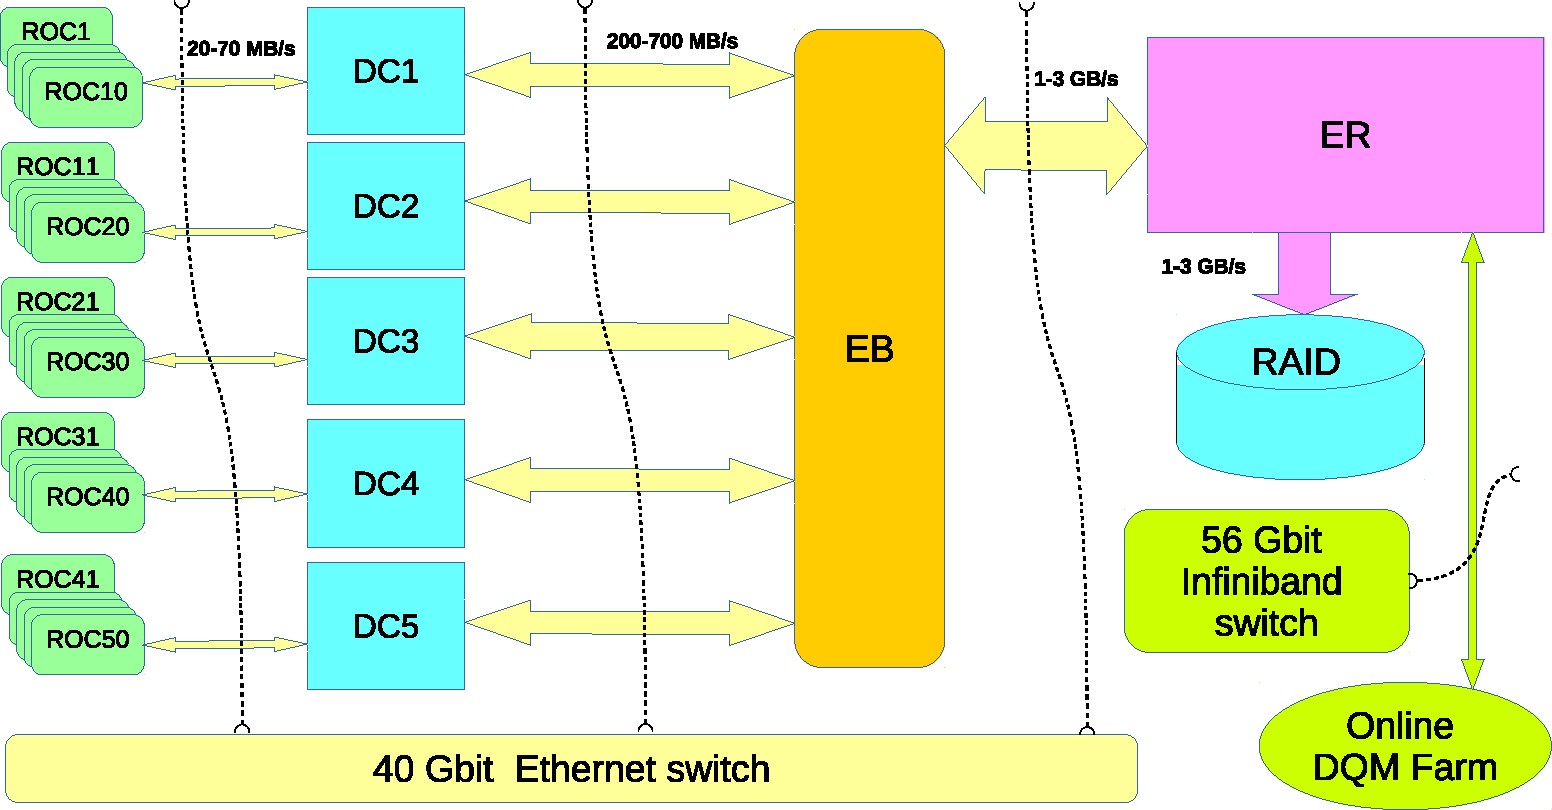
\includegraphics[width=0.75\textwidth]{figures/DAQ_coda.pdf}  
\caption{ \label{fig:CODA}
DAQ layout}

\end{center}
\end{figure}

%=======================+=========================
%================  Controls  ================
%=================================================

\section[Slow controls]{Slow controls \label{sec:controls}}
As any modern sophisticated particle detector system \gx{} requires being able to monitor 
and control tens of thousands of different variables that define the state of the experimental hardware. Different variable values need to be acquired, displayed, archived, used as inputs to control loops continually with a high degree of reliability. 

\subsection{Architecture \label{sec:controlsarchitechture}}
The \gx{} slow control system consists of three layers. The first layer consists of the remote units such as high voltage or low voltage power chassis, magnet power supplies, temperature controller, LabView applications, Programmable Logic Controller or PLC-based applications, which directly interact with the hardware and contain almost all of the control loops. The second layer is the Supervisory Control and Data Acquisition (SCADA) layer which is implemented in the form of EPICS\footnote{https://epics.anl.gov.} Input/Output Controllers or (IOC's). This layer provides the the interface between the low level application and the higher level applications using EPICS ChannelAccess protocol. The highest level, referred as Experiment Control System (ECS), contains the application such as Human-Machine Interface (HMI), the alarm system and data archiving. This structure allows for relatively easy and seamless addition and integration of new components into the overall controls system of \gx{}.    

\subsection{Remote Units \label{sec:controlsinterface}}
\gx{} uses a large number of commercial units that provide us with control over the hardware used in the experiment. For instance most of the detector high voltages are provided by the CAEN SYx527 voltage mainframe\footnote{https://www.caen.it/subfamilies/mainframes/} while the low and bias voltages are provided by boards residing in Wiener MPOD chassis\footnote{http://www.wiener-d.com/sc/power-supplies/mpod--lvhv/mpod-crate.html}. These two power supplies types provide most of the voltage with the exception of tagger microscope and forward calorimeter where custom systems were developed which provide voltage regulation and interact with EPICS-based layer through higher level interfaces using custom protocols, see Secs.~\ref{sec:TAGM} and \ref{sec:fcal} for more details.  

There are various beam line devices that need to be moved during beam operations. We use stepper motors to move these motorized stages via Newport XPS universal multi-axis motion controller\footnote{https://www.newport.com/c/xps-universal-multi-axis-motion-controller.} that allows for execution of complex trajectories involving multiple axes. All of the stage referencing, motion profile computations and encoder-based closed-loop control occur within the controller chassis after the basic parameters such as positions and velocities are provided by the user via TCP/IP based interface to EPICS.   

Often when installing complex systems, such as a superconducting magnet, we needed to develop a custom controls system with a large number of input, outputs channels and sophisticated logic suited for the particular system. For those cases we mostly  utilized Allen-Bradley CompactLogix and ControlLogix PLC systems\footnote{https://ab.rockwellautomation.com.}. These systems are designed for industrial systems that allow for a modular design and provide high reliability and require minimal maintenance. All of the controls loops are programmed within the PLC application. These types of PLC-s are interfaced with EPICS through TCP/IP EtherNet/IP proprietary protocol to allow the higher level applications access process variables served by the PLC-s.  

The cryogenic target and the superconducting solenoid magnet of \gx{} use National Instruments LabView applications. The controls of the target are done using custom-made and vendor-supplied hardware that include built-in remotely accessible control systems and a NI CompactRIO\footnote{https://www.ni.com/en-us/shop/compactrio.html} chassis that communicates with the hardware and serves the variables using internal ChannelAccess server and an EPICS IOC running on the CompactRIO controller, as described in details in Sec~\ref{sec:target}. We also use a National Instruments PXI high performance system\footnote{https://www.ni.com/en-us/shop/pxi.html} to collect data from different sensors as described in Sec.~\ref{sec:solenoid}. 

\subsection{Supervisory Control and Data Acquisition layer \label{sec:archiver}}
The Supervisory Control and Data Acquisition (SCADA) layer is the middle layer that distributes the process variables allowing the higher level, and sometimes lower level, applications to use various process variables of Hall D controls system. This layer is based on EPICS and uses ChannelAccess protocol to publish the values of the variables over Ethernet. And because the accelerator controls also uses EPICS, this allows us to efficiently exchange the information between the experiment and the accelerator operations. There are a few dozens of software Input/Out Controller (IOC) processes running on the hosts in the experiment control room that collect the data from different components of the lowest layer. Each of these IOC-s is configured to be able to communicate using the protocol appropriate for the remote units from which it needs to to exchange data. For instance the EPICS IOC controlling the voltage for the FDC detector needs to be able to communicate with Wiener MPOD and CAEN SYx527 voltage chassis. Although the middle layer is there mostly to distribute the data between different applications it also contains some EPICS-based applications running on IOC-s that provide different control loops and software interlocks.  For instance, the low voltage power supplies for the FDC detector (see Sec. \ref{sec:fdc}) are shut off if the temperature or the flow of the coolant in the chiller is out of required limits. 
\subsection{Experiment Control System \label{sec:alarms}}
The highest level of controls contains the applications that archive the data, display data in interactive GUIs and as stripcharts, alarm and notify shift personnel and experts in case problems occur, and also allow for interfacing with the CODA-based data acquisition system of \gx{} described is Sec.~\ref{sec:daq}.
The display management and the alarm system for \gx{} controls is based on Controls System Studio (CSS)\footnote{http://controlsystemstudio.org/}  which is an Eclipse-based toolkit for operating large systems and it is well suited for systems that use EPICS as its integral part. Although CSS provides its own archiving engine and stripcharting tools we utilized the MYA archiver~\cite{Slominski:2009icaleps} provided by the JLAB accelerator software group with its tools for displaying the archived data as time-series. The display management for \gx{} controls is done within CSS BOY~\cite{Chen:2011icaleps} environment that allows the system expert to build sophisticated control screen using standard widgets. The alarm system is based on CSS BEAST\cite{Kasemir:2009icaleps} alarm handler software which alerts the shift personnel about the problems with the detector and it also notifies the system expert if the problems are not resolved by the shift personnel in the experiments control room.   
%=======================+=========================
%================  Online  ================
%=================================================

\section[Online computing system (David)]{Online computing system \label{sec:online}}
\subsection{Monitoring \label{sec:onlinemonitoring}}
\subsection{Online event processing \label{sec:onlineprocessing}}


\clearpage   % avoid formatting problems with empty sections
%=======================+=========================
%================  Reconstruction  ================
%=================================================


\section[Event reconstruction (Alex A.)]{Event reconstruction \label{sec:reconstruction}}

% Copy from GlueX-doc-3108
% "Production and Analysis of GlueX Data"
% TODO: UPDATE for 2017

During and after experimental running, GlueX uses the computer center batch farm at Jefferson Lab to perform data monitoring, event reconstruction, and physics analyses.  For data monitoring, we study the detector hit occupancies, calibration and reconstruction quality, and experimental yields and resolutions for several physics channels.  We monitor a subset of the data as soon as it hits the tape, submitting batch farm jobs via cron job.  Every few weeks, we perform monitoring launches on a subset of the data to study improvements from ongoing calibrations and reconstruction software improvements.  The histograms produced by these monitoring jobs are published to the web, with the ROOT files available for download, so that collaborators can easily study the quality of the data. 

Every few months we perform a major reconstruction launch over all of the data, linking the hits in the various detector systems to reconstruct particles in the physics events.  Monitoring plots from these launches are also published to the web. Finally, about once a month we perform an analysis launch, where we run a collection of user-submitted analysis plugins over the reconstructed data, producing ROOT TTrees for further physics analysis. For all of these launches, we run JANA multithreaded to make efficient use of the available computing resources. %Figure~\ref{fig:offline_monitorA} shows the multithreaded scaling from our monitoring launches is near the theoretical limit.  SWIF is used to manage the batch farm jobs, and is queried to study the performance of the launches.  Figure~\ref{fig:farm-time} shows how many batch farm jobs were in each processing state as function of time our latest reconstruction launch.
The file outputs from these launches are written to the write-through cache, where they are pinned for further use and backed up to tape.  

Production of GlueX data is carried out in a series steps which we will describe for our first physics run. During the Spring 2017 beam time, GlueX recorded more than 1000 separate runs with a unique run number, which have a total data footprint of about one petabyte (check!). These data were collected in $19$ gigabyte files, with all physics quality runs consisting of multiple files (typically $100$ or more). Figure~\ref{fig:production_overview} shows an overview of the different production runs over GlueX data. 

\begin{figure}[h!]\centering
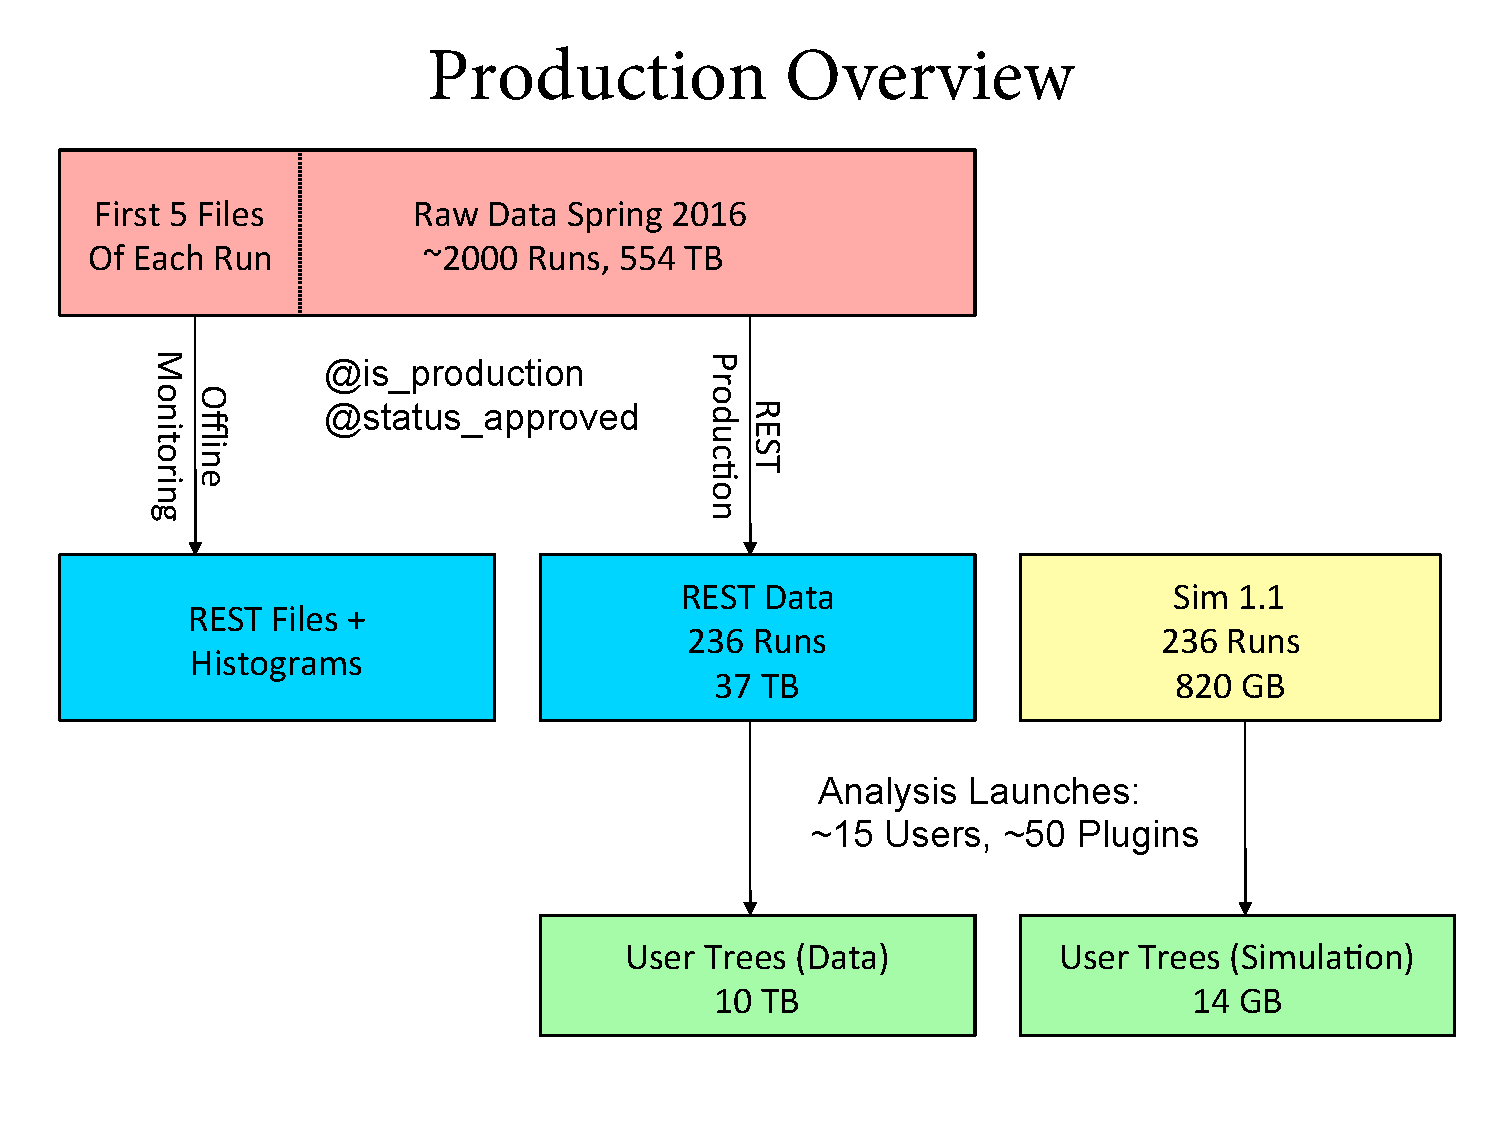
\includegraphics[width=0.8\textwidth]{figures/Production_Spring_2016.pdf}
\caption[]{\label{fig:production_overview}Production flow chart for GlueX data for the Spring 2016 
Engineering run.} 
\end{figure}

\subsection{Calibration pass \label{sec:reccalibration}}

Two types of calibration jobs are running, depending on the complexity of the calibration procedures.  Simple, well-understood calibrations such as timing alignment between individual channels and subdetectors or drift chamber gain and time-to-distance calibrations, can be performed with one file of data per run.  These procedures are run either in the online environment or on the batch farm, and can be run several times as needed due to improvements in reconstruction algorithms or other calibrations.

More complicated calibration procedures, such as calorimeter gain calibration, require more data and are often iterative procedures, requiring several passes through the available data.  The raw data is processed on the batch farm as it comes into the computer center to produce the outputs needed for these procedures, either in the form of histograms or reduced skims in EVIO or ROOT tree format.  Many of these output require that charged particle tracks be reconstructed, but because of the computationally intensive nature of track reconstruction at GlueX, the available computing resources at JLab are insufficient for fully reconstructing all of the raw data as it comes in.  Therefore, only about $10-20$\% of the data has the full suite of calibration procedures applied.  The rest has a limited set of procedures, mostly focused on separating out events collected by specialized triggers. 
The individuals responsible for specific detector calibrations are then responsible for analyzing the skimmed data.

\subsection{Monitoring pass \label{sec:recmonitoring}}

The red-colored box at the top represents the experimental data that has been copied to the computer center. The small part of the box represents the first five files of each run, which are run through the offline monitoring processes, see section~\ref{sec:onlinemonitoring}. These monitoring jobs are first run during the run to check the quality of the data, but are also run after major changes to calibrations or software to validate those changes. These jobs produce both Reconstructed Events Storage (REST) files and root histogram files for checking job performance.

\subsection{Reconstruction pass \label{sec:recreconstruction}}

We also carry out full production of physics quality data. In the physics data set, about 350 of the
runs were deemed physics quality. The remaining were short runs which were related to engineering and commissioning tests of the experiment. We note that while this number is small compared to the total number of runs, it is the vast majority of all data recorded during the running period, representing about $800$ (??) terabytes of data. All of these files are reconstructed and produce more than $100$ terabytes of REST data files. The large reduction is size from collected event data to physics data files allows us to  more quickly and efficiently carry out physics analyses on the data.
%, and is also small enough to be fully exported to off-site computer centers, see section~\ref{sec:remote-dist} (not really).

In the REST production, we included a series of detector performance studies that required access to raw data and would not be possible on the reconstructed data alone. Many improvements to software and detector calibration resulted from these studies. Similar studies can be made with simulated data to match and assess the detector acceptance.

\subsection{Offsite Reconstruction}
\label{sec:recoffsite}

\subsection{Analysis pass \label{sec:recanalysis}}

The reconstructed (REST) data is also skimmed to produce working data sets for physics. This needs more description here and is represented by the left-hand
green box at the bottom of Figure~\ref{fig:production_overview}. Users submit skim code as an \emph{analysis plugin} and it is connected to the master skim job that runs at Jefferson Lab. The skim job shown here had $50$ of these plug-ins and produced about $10$ Terabytes of root files for detailed physics analysis. The volume of these root files is dependent on the number of plug-ins.

%=======================+=========================
%================  Simulation  ================
%=================================================


\section{Monte Carlo simulation \label{sec:simulation}}
\subsection{Event generators \label{sec:generators}}
\subsection{HDGeant \label{sec:hdgeant}}
\subsection{Material thickness scan \label{sec:materialscan}}
\subsection{Job submission \label{sec:jobsubmission}}


%=======================+=========================
%================  Performance  ================
%=================================================

\section[Detector performance (Sean)]{Detector performance \label{sec:performance}}

\subsection{Kinematic fitting \label{sec:perffitting}}

\subsection{Charged particles \label{sec:perfcharged}}

\subsubsection{Resolution \label{sec:perfchargedresol}}

\subsubsection{Efficiency \label{sec:perfchargedeff}}

\subsection{Neutral particles \label{sec:perfneutral}}

\subsubsection{Resolution \label{sec:perfneutralresol}}

\subsubsection{Efficiency \label{sec:perfneutraleff}}

\subsection{Particle identification \label{sec:perfpid}}

\subsection{Systematic uncertainties \label{sec:systematics}}

\input{summary}   

%================+===================
%========  Acknowledgments  =========
%====================================

\section{Acknowledgments}   
***DRAFT modified from eta eta' paper***\\
We would like to acknowledge the outstanding efforts of technical support at all the collaborating institutions and the support groups at Jefferson Lab that completed the assembly, installation
and assist with the maintenance of the detector. This work was  supported by the Natural Sciences and Engineering Research Council of Canada grant SAPPJ-2018-00021 and by the U.S. Department of Energy, Office of Science, Office of Nuclear Physics under contract DOE Grant No. DE-FG02-87ER40315.  This work was also supported in part by the U.S. Department of Energy, the U.S. National Science Foundation, the German Research Foundation, GSI Helmholtzzentrum f\"{u}r Schwerionenforschung GmbH, the Russian Foundation for Basic Research, the UK Science and Technology Facilities Council, the Chilean Comisi\'{o}n Nacional de Investigaci\'{o}n Cient\'{i}fica y Tecnol\'{o}gica, the National Natural Science Foundation of China, and the China Scholarship Council. This material is based upon work supported by the U.S. Department of Energy, Office of Science, Office of Nuclear Physics under contract DE-AC05-06OR23177. 

\newpage

\section*{References}
   
%\nocite{*}
\bibliography{GlueX_nim}
\bibliographystyle{unsrt}
%\bibliographystyle{elsarticle-num}

\end{document}
